\section{Résumé en français}
%%%%%%%%%%%%%%%%%%%%%%%%%%%%%%%%%%%%%%%%%%%%%%%%%%%%%%%%%%%%%%%%%%%%%%%%%%%
%%%%%%%%%%%%%%%%%%%%%%%%%%%%%%%%%%%%%%%%%%%%%%%%%%%%%%%%%%%%%%%%%%%%%%%%%%%
Après avoir développé et analysé une simulation originale des grandes structures turbulentes dans le détroit de Gibraltar, dans le cinquième et dernier chapitre de ce manuscrit nous abordons la problématique de l'évaluation du mélange turbulent dans une simulation numérique des grandes structures turbulentes. La quantification et la localisation de ce mélange turbulent via celle des flux diapycnaux dans l'océan est un problème délicat.\\
Les premières pierres d'un cadre théorique rigoureux ont en effet été posées il y a maintenant plus d'un demi-siècle par E. Lorenz \citep{lorenz_available_1955} avant qu'un algorithme simple ne soit proposé à la fin du siècle précédent par \cite{winters_available_1995} à partir d'une analyse appuyée sur une raisonnement très physique. La simplicité de cette application algorithmique en fait la force mais aussi d'une certaine façon la faiblesse, en particulier à cause des hypothèses très fortes sur lesquelles elle est fondée. Une hypothèse simplificatrice centrale est celle de la constance du volume de fluide considéré, hypothèse qui devient problématique lorsque le domaine considéré pour le bilan d'énergie potentielle est constitué de colonnes d'eau de mer dont la surface libre et donc la hauteur évoluent au cours du temps.

\color{blue}
Dans le chapitre \ref{chapBPE}, une équation d'évolution complète est tout d'abord proposée pour l'énergie potentielle, l'équation proposée intègre en particulier la somme des contributions de la variation de surface en $dz^*/dt$ ($z^*(\rho)$ représentant ici la cote d'une particule de masse volumique $\rho$ dans le profil de référence réarrangé. A partir de cette équation d'évolution, l'algorithme classique proposé par \cite{winters_available_1995} est généralisé à une somme de colonnes océaniques: une diffusivité efficace est ainsi calculée à partir d'un bilan complet d'énergie potentielle (plus spécifiquement d'énergie potentielle de référence ou BPE en anglais) via la relation \ref{eq_kappaEff}.

Cet algorithme généralisé est ensuite appliqué à un ensemble de configurations de complexité croissante, chaque configuration permettant d'analyser et d'évaluer la pertinence de la quantification et de la localisation du mélange turbulent. Une équation d'advection-diffusion d'un traceur passif est tout d'abord étudiée dans le cadre de stratifications linéaires puis "bi-couche". Le mélange induit par les oscillations libres d'une cuve stratifiée ou le mélange induit dans un écoulement bi-couche instable ou par un écoulement dans la région du détroit de Gibraltar est lui-aussi analysé. Ces trois dernières configurations sont simulées numériquement avec le code océanique à toit libre CROCO dans sa version compressible et non-hydrostatique.

Une première conclusion est que la généralisation de l'algorithme de \cite{winters_available_1995} permet une évaluation rigoureuse et "suffisamment" précise du mélange turbulent (comparée aux erreurs induites par son évaluation). L'efficacité de l'algorithme doit toutefois encore être optimisée avant que ce dernier ne soit appliqué à très haute résolution à des régions océaniques d'extension conséquente.

%%%%%%%%%%%%%%%%%%%%%%%%%%%%%%%%%%%%%%%%%%%%%%%%%%%%%%%%%%%%%%%%%%%%%%%%%%%
\section{Introduction}
%%%%%%%%%%%%%%%%%%%%%%%%%%%%%%%%%%%%%%%%%%%%%%%%%%%%%%%%%%%%%%%%%%%%%%%%%%%

In the present chapter \ref{chapBPE}, a substantial step is made toward the quantification of mixing in realistic ocean configurations. The objective is to generalize \citet{winters_available_1995}'s framework to the real ocean made of volume-varying ocean columns.

%the determination of the reference profile $z^*(\rho)$ to this evolution equation, as a tool to evaluate the turbulent mixing in realistic ocean configurations.
\color{blue} Following \cite{lorenz_available_1955} and in a fully compressible context, \cite{tailleux_energetics_2009} and lately \cite{tailleux_irreversible_2013} derived a rigorous (conceptual) thermodynamic framework to study the available potential energy (APE), defined as the difference between the potential energy (PE) and the potential potential energy (BPE). The latter BPE potential energy compartment is defined with respect to a "reference" state, often called a \textit{Lorenz reference state} \citep{saenz_estimating_2015}. \cite{winters_available_1995} proposed an algorithm to compute (i) this reference state by an adiabatic reorganisation of the fluid density, (ii) an approximation of the diffusivity responsible for diapycnal mixing for a constant-volume region.

Under a Boussinesq approximation, local expressions of the available potential energy have ever since been derived \citep{winters_available_2013}. Lately \cite{howland_mixing_2020,howland_quantifying_2020} quantifyed both mixing and available potential energy in vertically periodic simulations of a stratified flow, making a first step toward domains with varying vertical boundaries. However \cite{saenz_estimating_2015} and, more recently, Tailleux in his latest publications \citep{tailleux_local_2018} insist on the fact that Lorenz reference state is difficult to define and compute. As a consequence, their studies are dedicated to the evaluation of the errors and discrepancies when simpler and easier-to-obtain reference states are defined (as, for instance, horizontal averaged).\color{black}

\color{blue}To take into account the potential evolution in time of the volume (and as a consequence of the potential energy) of water columns due to free-surface anomalies, a general evolution equation for the Background Potential Energy (BPE) needs to be derived.
%In addition to the evaluation of several new terms in the evolution equation, 
Based on such an evolution equation, \cite{winters_available_1995}'s algorithm can then be generalized to realistic numerical ocean configurations. To do so, additional difficulties needs to be solved in order to take into account: (i) bathymetry variations, (ii) variations of grid-cell volume in terrain-following s-coordinates, and (iii) diffusive and advective fluxes through open boundaries. In particular for this last point, diapycnal fluxes associated in fine to mixing are known to be several orders of magnitude smaller than advective fluxes associated for instance to ocean tides, and computation of the term of the balance equation must be carried out while preserving a high accuracy.

%Propositions are made to overcome such algorithmic difficulties and a step is made toward an original evaluation of mixing in realistic ocean configurations.
The generalized algorithm proposed hereafter consequently takes root in the "milestone" publication by \citet{winters_available_1995}. Lately \citet{saenz_estimating_2015} and \citet{tailleux_local_2018} proposed more efficient algorithms for the determination of the reference profile (see \S \ref{section_PE_chap2} of the manuscript for a review). These modifications have not yet been implemented because (i) the cases studied so far do not require too large computations, and (ii) \citet{winters_available_1995}'s approach is to be used as a reference and, as a consequence, needs to be first implemented. The aim of this chapter is not only to evaluate the relevance and efficiency of the method but also to point where the approach needs to be further refined.

In this chapter, we first propose an extension of \cite{winters_available_1995}'s algorithm to a free-surface, non-flat ocean in section \ref{BPE_algo}. It is applied first in section \ref{section_numlab} to a simple advection - diffusion equation using homogeneous grid cells. In a second step, CROCO ocean model is implemented in test-case configurations of section \ref{section_CROCO_BPE}. Those configurations are of increasing complexity in term of bathymetry and dynamics; the last, more realistic configuration being the vertical section of Gibraltar Experiment (SimRef) studied in chapter \ref{chapGBR2D}.

%With this original algorithm, we investigate, quantify and localize the turbulent mixing induced when a simple passive tracer is (numerically) advected by a constant current and diffused at a constant (known) rate. In the last section, the turbulent mixing induced in an oscillating tank, in an area of ocean submitted to Kelvin-Helmholtz instabilities and in the region of the strait of Gibraltar is studied.
\color{blue}
\section{Mixing in a general volume-varying ocean region}
\subsection{Decomposition of potential energy balance in a free-surface ocean}
\label{section_PE_chap2}

The \textit{ocean model} proposed and detailed so far is self-consistent and can lead to the description of numerous dynamical processes over a wide range of space-time scales. To proceed, one needs to develop dedicated diagnostics and to focus on the mechanisms of particular interest. In this context, a central objective of the present study is to explicitly simulate large turbulent eddies in order to improve the representation of the transformation of water masses. In other words, the (implicit) modeling or the (explicit) simulation of \textit{mixing} is at stake.

The most rigorous approach of the \textit{mixing}-related issues has undoubtedly been proposed by \cite{lorenz_available_1955}. It is based on the concept of Background and Available gravitational Potential Energy (hereafter respectively BPE and APE) as a decomposition of the total gravitational Potential Energy (PE). The author defines first APE as the potential energy released when reorganizing adiabatically the flow so that it reaches its state of minimal potential energy. This minimal value corresponds to the BPE, that can also be expressed as the difference between the PE and the APE. The BPE compartment, thus defined, grows monotonically under diabatic mixing, offering a well-defined tool to evaluate this mixing.

Lorenz' approach, popularized by \cite{winters_available_1995}, remains challenging when applied in a realistic context, for instance over a limited area of a free-surface, varying-bathymetry ocean. It is even more challenging if applied in a numerical context with a s-coordinate model. A "limited area" raises indeed many questions on boundary fluxes and the validity of the state of minimal energy, whereas a free surface or a varying bathymetry both complicate the computation of this state in particular when s-coordinates are used.

As a consequence, localization and furthermore the accurate evaluation of hot spots of enhanced mixing in the context of the \textit{ocean model} presented so far remain a challenge. A general formulation of the evolution equation of both the PE and BPE is now proposed for a given volume made of water columns that expand vertically with the movements of the free-surface. The relations thus obtained are then used to characterize the mixing in various configurations of ocean regions in chapter \ref{chapBPE}.


\subsubsection{Reference state(s)}

The state of the stratification after the adiabatical reorganization of \citet{lorenz_available_1955} is called the Lorenz reference state. It consists in attributing a reference depth $z^*$ to each fluid parcel, the potential energy of this state, the BPE, can then be expressed as :
\begin{equation}
    E_b = \int_x \int_{-1}^0 g \rho z^* dx ds
\end{equation}
The evolution of BPE, through the evolution of the stratification profile $z^*$, reflects the adiabatic mixing processes that can then be quantified.

However, both \cite{saenz_estimating_2015} and \cite{tailleux_local_2018} insist on the fact that this Lorenz reference state of absolute minimum potential energy is difficult to define and compute (due to numerical cost of sorting algorithm, non-linearity of the EOS, etc.). As a consequence, these studies are dedicated to the evaluation of the errors and discrepancies when simpler and easier-to-obtain reference states are defined (horizontal averaged, etc.). \cite{saenz_estimating_2015} additionally describes in detail an algorithm to compute Lorenz' reference state in an efficient way. They associate the computation of $Z^*(\rho)$ from the computation of the Level of Neutral Buoyancy (their LNB) and they separate it from the computation of Lorenz' reference state that is obtained first by inverting a non-linear relation. This algorithm is claimed to be much more efficient than classical adiabatic redistribution algorithms based on \citet{winters_available_1995}.

%Beyond the definition of a reference state and more precisely beyond the definition of a reference profile, several underlying ideas can be found:
%\begin{itemize}
%\setlength\itemsep{0pt}
%	\item The reference state is a basic (not necessarily resting but possibly balanced) state to which full dynamics is to be compared.
%	\item The Boussinesq assumption is itself based on the choice of a reference (constant) density (usually named here $\tilde{\rho}_{0}$) that is subtracted from the 3D total density. An hydrostatic pressure $p_{00}$ is defined by $\partial p_{00}/ \partial z=-\tilde{\rho}_{0} g$. Subtracting directly a vertically-varying reference density $\tilde{\rho}_{0}(z)$ leads to the less restrictive anelastic assumption. Interestingly enough, this Boussinesq reference state $(\tilde{\rho}_{0},\ p_{00})$ can be associated to the thermodynamic equilibrium state. \cite{tailleux_energetics_2009,tailleux_thermodynamicsdynamics_2012} associates this reference state to the \textit{internal dead energy} compartment (named $IE0$) concluding that "the viscous dissipation of kinetic energy (hereafter KE) and the diffusive dissipation of APE" increase the reference temperature $T_{00}$ (decreasing $\tilde{\rho}_{0}$) by increasing the IE0 (page 9 of the latter publication).
%	\item The reference profile (named here $\rho_0$) with both time and space (vertical) dependencies is then defined by $\rho(t,\mathbf{x})=\tilde{\rho}_{0}+\rho_0(t,z)+\rho'(t,\mathbf{x})$.  \cite{tailleux_thermodynamicsdynamics_2012} (still page 9) further claims that "turbulent mixing smooths out the vertical gradient of $\rho_0(t,z)$ after defining the exergy compartment of the internal energy. An hydrostatic pressure component $p_0$ can then be defined in association with $\rho_0$.
%	\item The reference state $\rho_0(t,z)$ is additionally used by \citet{andrews_note_1981} and \citet{tailleux_local_2018} to decompose the available potential energy into its elastic and potential compartments. This is done by defining two states. A transformation can be applied to a given fluid volume in such a way that its entropy, salinity and pressure $(\eta,S,p)$ themselves transformed (i) into $(\eta,S,\tilde{p}_0(t,z))$ (changing the reference pressure at $(t,z)$ while keeping $\eta$ and $s$ constant) and (ii) into $(\eta,S,p_0(z_r))$ (transferring the particulate to its "Level of Neutral Buoyancy" (LNB) given by $z=z_r$ while keeping $\eta$ and $S$ constant. 
%%\textit{Link to be studied with \cite{mcdougall_potential_2003}'s conservation of potential enthalpy}.
%\end{itemize}
It is crucial to know what state of the ocean a given reference state relates to in order to work within the BPE framework. 

%%%%%%%%%%%%%%%%%%%%%%%%%%%%%%%%%%%%%%%%%%%%%%%%%%%%%%%%%%%%%%%%%%%%%%%%%%%%%
\subsection{Balance of PE in s-coordinates}
%%%%%%%%%%%%%%%%%%%%%%%%%%%%%%%%%%%%%%%%%%%%%%%%%%%%%%%%%%%%%%%%%%%%%%%%%%%%%
The evolution of the specific PE can be obtained from the general evolution equation in s-coordinates derived in Appendix \ref{sub_conservation_ins} 
by setting $A=gz$ :
%\paragraph{Potential energy}
\begin{subequations}
  \begin{alignat}{2}
  \displaystyle 
 	&\frac{d E_p}{d t}  &&=g\int_x \int_{-1}^0 \frac{\partial \rho h z}{\partial t}\bigg\rvert_{s} dx ds 
  \end{alignat}
\end{subequations}
Replacing $A$ in expression \ref{Aint}, that uses the evolution equation for density \ref{eq_diff_cart} :
\begin{subequations}
  \begin{alignat}{2}
  \displaystyle 
 %
 % Begin 2nd line
 %
 &\frac{d E_p}{d t}   &&= \quad  g\int_x \int_{-1}^0 \rho h \frac{\partial z}{\partial t}\bigg\rvert_{xs} \ dx ds\\[4mm]
 %
 & && \quad - g\bigg[ \int_{-1}^0 \rho h z u \ ds\bigg]_{x}
 + g\int_x \int_{-1}^0\rho h u \frac{\partial z}{\partial x}\bigg\rvert_{ts} \ dx ds\\[4mm] 
 & && \quad - g\bigg[ \int_x \frac{\partial \rho z v_s}{\partial s}\bigg\rvert_{tx} \ dx\bigg]_0^1
 + g\int_x \int_{-1}^0 \rho v_s \frac{\partial z}{\partial s}\bigg\rvert_{tx} \ dx ds \\[4mm]
 & && \quad + g\bigg[ \int_{-1}^0 h z \kappa^h \frac{\partial \rho}{\partial x}\bigg\rvert_{ts} \ ds \bigg]_{x}
 - g\int_x \int_{-1}^0 h \kappa^h \frac{\partial z}{\partial x}\bigg\rvert_{ts} \frac{\partial \rho}{\partial x}\bigg\rvert_{ts} \ dx ds \\[4mm]
 & && \quad + g\bigg[ \int_x z \frac{\kappa^v}{h} \frac{\partial \rho}{\partial s}\bigg\rvert_{tx} \ dx \bigg]_0^1
 - g\int_x \int_{-1}^0 \frac{\kappa^v}{h} \frac{\partial z}{\partial s}\bigg\rvert_{tx} \frac{\partial \rho}{\partial s}\bigg\rvert_{tx} \ dx ds
  \end{alignat}
\end{subequations}
The advective flux of PE (fourth term at the RHS) can be integrated by part leading to:

\begin{subequations}
  \begin{alignat}{2}
  \displaystyle 
 	&\frac{d E_p}{d t}  &&= \quad  \underbrace{g\int_x \int_{-1}^0 \rho h \frac{\partial z}{\partial t}\bigg\rvert_{xs} \ dx ds}_{(1)}\\[4mm]
  %
 & && \quad - g\bigg[ \int_{-1}^0 \rho h z u \ ds\bigg]_{x}
 + \underbrace{g\int_x \int_{-1}^0\rho h u \frac{\partial z}{\partial x}\bigg\rvert_{ts} \ dx ds}_{(2)}\\[4mm] 
 & && \quad - \underbrace{g\bigg[ \int_x\rho z v_s \ dx\bigg]_0^1}_{=0}
 + \underbrace{g\int_x \int_{-1}^0 \rho h v_s \ dx ds}_{(3)} \\[4mm]
 & && \quad + g\bigg[ \int_{-1}^0 h z \kappa^h \frac{\partial \rho}{\partial x}\bigg\rvert_{ts} \ ds \bigg]_{x} 
 - g\int_x \int_{-1}^0 h \kappa^h \frac{\partial z}{\partial x}\bigg\rvert_{ts} \frac{\partial \rho}{\partial x}\bigg\rvert_{ts} \ dx ds \\[4mm]
 & && \quad + g\bigg[ \int_x z \frac{\kappa^v}{h} \frac{\partial \rho}{\partial s}\bigg\rvert_{tx} \ dx \bigg]_0^1
 - g\int_x \int_{-1}^0 \kappa^v \frac{\partial \rho}{\partial s}\bigg\rvert_{tx} \ dx ds 
  \end{alignat}
\end{subequations}
where the advection of PE at the surface and at the bottom vanishes. At the RHS, terms (1), (2) and (3) can be gathered to recover the buoyancy flux component $(\phi_z)$ of \citet{winters_available_1995}.
\begin{subequations}
  \begin{alignat}{2}
  \displaystyle 
 	&\frac{d E_p}{d t}  &&= \quad  \underbrace{\int_x \int_{-1}^0 \rho g h v_z \ dx ds}_{=(1)+(2)+(3)\equiv\phi_z}\\[4mm]
 %
 & && \quad - g\bigg[ \int_{-1}^0 \rho h z u \ ds\bigg]_{x}\\[4mm] 
 & && \quad + g\bigg[ \int_{-1}^0 h z \kappa^h \frac{\partial \rho}{\partial x}\bigg\rvert_{ts} \ ds \bigg]_{x}
 - g\int_x \int_{-1}^0 h \kappa^h \frac{\partial z}{\partial x}\bigg\rvert_{ts} \frac{\partial \rho}{\partial x}\bigg\rvert_{ts} \ dx ds \\[4mm]
 & && \quad + g\bigg[ \int_x z \frac{\kappa^v}{h} \frac{\partial \rho}{\partial s}\bigg\rvert_{tx} \ dx \bigg]_0^1
 - g\int_x \int_{-1}^0 \kappa^v \frac{\partial \rho}{\partial s}\bigg\rvert_{tx} \ dx ds
  \end{alignat}
\end{subequations}
%%%%%%%%%%%%%%%%%%%%%%%%%%%%%%%%%%%%%%%%%%%%%%%%%%%%%%%%%%%%%%%%%%%%%%%%%%%%%
%\paragraph{Background Potential energy}
%%%%%%%%%%%%%%%%%%%%%%%%%%%%%%%%%%%%%%%%%%%%%%%%%%%%%%%%%%%%%%%%%%%%%%%%%%%%%

%%%%%%%%%%%%%%%%%%%%%%%%%%%%%%%%%%%%%%%%%%%%%%%%%%%%%%%%%%%%%%%%%%%%%%%%%%%%%
\subsection{Balance of BPE in s-coordinates}
%%%%%%%%%%%%%%%%%%%%%%%%%%%%%%%%%%%%%%%%%%%%%%%%%%%%%%%%%%%%%%%%%%%%%%%%%%%%%
The same relation \ref{Aint} derived in Appendix \ref{sub_conservation_ins} can alternatively be used for $A=gz^*$, the specific BPE, leading to:
\begin{subequations}
\label{eq_evolBPE0}
  \begin{alignat}{2}
  \displaystyle 
 	&\frac{d E_b}{d t} &&=
 	g\int_x \int_{-1}^0 \frac{\partial \rho h z^*}{\partial t}\bigg\rvert_{s} \ dx ds
  \end{alignat}
\end{subequations}
and then 	
\begin{subequations}
  \begin{alignat}{2}
  \displaystyle 
 %
 % Begin 2nd line
 %
 & \frac{d E_b}{d t} &&= \quad  {g\int_x \int_{-1}^0 \rho h \frac{\partial z^*}{\partial t}\bigg\rvert_{xs} \ dx ds}_{(1)}\\[4mm]
  %
 & && \quad - g\bigg[ \int_{-1}^0 \rho h z^* u \ ds\bigg]_{x}
 + {g\int_x \int_{-1}^0\rho h u \frac{\partial z^*}{\partial x}\bigg\rvert_{ts} \ dx ds}_{(2)}\\[4mm] 
 & && \quad - 0
 + {g\int_x \int_{-1}^0 \rho v_s \frac{\partial z^*}{\partial s}\bigg\rvert_{tx} \ dx ds}_{(3)} \\[4mm]
 & && \quad + g\bigg[ \int_{-1}^0 h z^* \kappa^h \frac{\partial \rho}{\partial x}\bigg\rvert_{ts} \ ds \bigg]_{x}
 - g\int_x \int_{-1}^0 h \kappa^h \underbrace{\frac{\partial z^*}{\partial x}\bigg\rvert_{ts} }_{=\frac{d z^*}{d\rho}\frac{\partial \rho}{\partial x}\big\rvert_{ts}\color{black}}\frac{\partial \rho}{\partial x}\bigg\rvert_{ts} \ dx ds \\[4mm]
 & && \quad + g\bigg[ \int_x z^* \frac{\kappa^v}{h} \frac{\partial \rho}{\partial s}\bigg\rvert_{tx} \ dx \bigg]_0^1
 - g\int_x \int_{-1}^0 \frac{\kappa^v}{h} \frac{\partial z^*}{\partial s}\bigg\rvert_{tx} \frac{\partial \rho}{\partial s}\bigg\rvert_{tx} \ dx ds
  \end{alignat}
\end{subequations}
The terms associated to the particulate derivative of $z^*$ can be gathered from terms (1), (2) and (3):
%\begin{subequations}
%  \begin{alignat}{2}
%  \displaystyle 
% 	&\frac{d E_b}{d t}  &&= \quad g\int_x \int_{-1}^0 \rho h \frac{\partial z^*}{\partial t}\bigg\rvert_{xs}
% +\rho v_s \frac{\partial z^*}{\partial s}\bigg\rvert_{tx} 
%+\rho h u \frac{\partial z^*}{\partial x}\bigg\rvert_{ts} \ dx ds \\[4mm]
% & && \quad - g\bigg[ \int_{-1}^0 \rho h z^* u \ ds\bigg]_{x}\\[4mm] 
% & && \quad - 0 \\[4mm]
% & && \quad + g\bigg[ \int_{-1}^0 h z^* \kappa^h \frac{\partial \rho}{\partial x}\bigg\rvert_{ts} \ ds \bigg]_{x}
% - g\int_x \int_{-1}^0 h \kappa^h \frac{d z^*}{d \rho} \frac{\partial \rho}{\partial x}\bigg\rvert_{ts}^2 \ dx ds \\[4mm]
% & && \quad + g\bigg[ \int_x z^* \frac{\kappa^v}{h} \frac{\partial \rho}{\partial s}\bigg\rvert_{tx} \ dx \bigg]_0^1
% - g\int_x \int_{-1}^0 \frac{\kappa^v}{h} \frac{d z^*}{d \rho} \frac{\partial \rho}{\partial s}\bigg\rvert_{tx}^2 \ dx ds
%  \end{alignat}
%\end{subequations}
%to explicitly express $dE_b/dt$ as a function of $dz^*/dt$:
\begin{subequations}
\label{eq_evolBPE}
  \begin{alignat}{2}
  \displaystyle 
 	&\frac{d E_b}{d t}  &&= \quad \underbrace{g\int_x \int_{-1}^0 \rho h \frac{d z^*}{d t}\ dx ds }_{(1)+(2)+(3)}\\[4mm]
 & && \quad - \underbrace{g\bigg[ \int_{-1}^0 \rho h z^* u \ ds\bigg]_{x}}_{\approx S_{adv}}\\[4mm] 
 & && \quad + \underbrace{g\bigg[ \int_{-1}^0 h z^* \kappa^h \frac{\partial \rho}{\partial x}\bigg\rvert_{ts} \ ds \bigg]_{x}}_{S_{diff}^{(h)}}
 \underbrace{- g\int_x \int_{-1}^0 h \kappa^h \frac{d z^*}{d \rho} \frac{\partial \rho}{\partial x}\bigg\rvert_{ts}^2 \ dx ds}_{\phi_d^{(h)}} \\[4mm]
 & && \quad + \underbrace{g\bigg[ \int_x z^* \frac{\kappa^v}{h} \frac{\partial \rho}{\partial s}\bigg\rvert_{tx} \ dx \bigg]_0^1}_{S_{diff}^{(v)}}
 \underbrace{- g\int_x \int_{-1}^0 \frac{\kappa^v}{h} \frac{d z^*}{d \rho} \frac{\partial \rho}{\partial s}\bigg\rvert_{tx}^2 \ dx ds}_{\phi_d^{(v)}}
  \end{alignat}
\end{subequations}
%Substituting $hdz^*/dt$ by the product of $dz^*/d\rho$ by $hd\rho/dt$ leads to\color{red}(en a besoin?)\color{black}:
%\begin{subequations}
%  \begin{alignat}{2}
%  \displaystyle 
% 	&\frac{d E_b}{d t}  &&= \quad \underbrace{g\int_x \int_{-1}^0  
% \rho  \frac{d z^*}{d\rho} \bigg[h \color{black}
% \frac{\partial \rho}{\partial t}\bigg\rvert_{xs} 
% +\rho v_s \frac{\partial \rho}{\partial s}\bigg\rvert_{tx} 
%+\rho h u \frac{\partial \rho}{\partial x}\bigg\rvert_{ts}
%\bigg] \ dx ds}_{(1)}\\[4mm]
% & && \quad - \underbrace{\bigg[ \int_{-1}^0 \rho g h z^* u \ ds\bigg]_{x}}_{\approx S_{adv}}\\[4mm] 
% & && \quad + \underbrace{g\bigg[ \int_{-1}^0 h z^* \kappa^h \frac{\partial \rho}{\partial x}\bigg\rvert_{ts} \ ds \bigg]_{x}}_{S_{diff}^{(h)}}
% - \underbrace{g\int_x \int_{-1}^0 h \kappa^h \frac{d z^*}{d \rho} \frac{\partial \rho}{\partial x}\bigg\rvert_{ts}^2 \ dx ds}_{\phi_d^{(h)}} \\[4mm]
% & && \quad +\underbrace{ g\bigg[ \int_x z^* \frac{\kappa^v}{h} \frac{\partial \rho}{\partial s}\bigg\rvert_{tx} \ dx \bigg]_0^1}_{S_{diff}^{(v)}}
% - \underbrace{g\int_x \int_{-1}^0 \frac{\kappa^v}{h} \frac{d z^*}{d \rho} \frac{\partial \rho}{\partial s}\bigg\rvert_{tx}^2 \ dx ds}_{\phi_d^{(v)}}
% %
% % Begin 5th line
% %
%% & &&= \quad g\int_x \int_{-1}^0 \rho h \frac{\partial z^*}{\partial t}\bigg\rvert_{xz}
% %+\rho v_z \frac{\partial z^*}{\partial z}\bigg\rvert_{tx} 
%%+\rho h u \frac{\partial z^*}{\partial x}\bigg\rvert_{tz} \ dx ds \\
% %& && \quad - \bigg[ \int_{-1}^0 \rho g h z^* u \ ds\bigg]_{x}\\ 
%% & && \quad + g\bigg[ \int_{-1}^0 h z^* \kappa^h \frac{\partial \rho}{\partial x}\bigg\rvert_{ts} \ ds \bigg]_{x}
%% - g\int_x \int_{-1}^0 h \kappa^h \frac{\partial z^*}{\partial \rho} \frac{\partial \rho}{\partial x}\bigg\rvert_{ts}^2 \ dx ds \\
%% & && \quad + g\bigg[ \int_x z^* \frac{\kappa^v}{h} \frac{\partial \rho}{\partial s}\bigg\rvert_{tx} \ dx \bigg]_0^1
%% - g\int_x \int_{-1}^0 \frac{\kappa^v}{h} \frac{\partial z^*}{\partial \rho} \frac{\partial \rho}{\partial s}\bigg\rvert_{tx}^2 \ dx ds 
%  \end{alignat}
%\end{subequations}
where $S_{adv}$ is the lateral (horizontal) advective flux of BPE, $S^{(v)}_{diff}$ and $S^{(h)}_{diff}$ are the vertical and horizontal diffusive fluxes, $\phi^{(v)}_d$ and $\phi^{(h)}_d$ are the diapycnal vertical and horizontal fluxes.

%%%%%%%%%%%%%%%%%%%%%%%%%%%%%%%%%%%%%%%%%%%%%%%%%%%%%%%%%%%%%%%%%%%%%%%%%%%%%
\subsubsection{Time variations of $z^*$}
%%%%%%%%%%%%%%%%%%%%%%%%%%%%%%%%%%%%%%%%%%%%%%%%%%%%%%%%%%%%%%%%%%%%%%%%%%%%%
The first RHS term of equation \ref{eq_evolBPE}, 

\begin{equation}
\label{RHS_BPE_1}
g\int_{x} \int_{-1}^0 \rho h \frac{d z^*}{d t}\ dx ds \\
\end{equation}

is akin to a vertical buoyancy-flux term for the $z^*$ reference state. It vanishes for a volume of integration with fixed-in-time boundaries (\cite{winters_available_1995}, \cite{huang_mixing_1998} and many others...). But it has no particular reason to vanish when movements of the free-surface are taken into account. This paragraph constitutes a proposition for its development in this case.

Going back to a more general notation of our integral volume $V_{\zeta}$ and following \citet{huang_mixing_1998}, $z^*$ can be expressed as a function of the volume $v(\rho)$ of fluid with a density larger than $\rho$ :
%En annexe de \citep{huang_mixing_1998}, on peut exprimer $z^*$ fonction de $v(\rho)$ le volume des parcelles de densité supérieures ou égales à $\rho$ :
\begin{equation}
v(\rho)=\iiint_{\zeta} H(\rho(\mathbf{x}',t)-\rho(\mathbf{x},t))d\mathbf{x}' %= \int_x\int_{-1}^0 H(\rho(x',s',t)-\rho(x,s,t))h ds'dx'
\end{equation}
where $H$ is the Heaviside function, equals to 0 for $\rho(\mathbf{x}',t)<\rho(\mathbf{x},t)$, $1/2$ for $\rho(\mathbf{x}',t)=\rho(\mathbf{x},t)$ , and 1 for $\rho(\mathbf{x}',t)>\rho(\mathbf{x},t)$.

In the reference profile, a given density is associated to a reference depth. This volume can then be expressed as $v(z^*)$, the volume of water between the bottom and the $z^*$ level in the water column :
\begin{equation}
v(z^*)=\int^{z^*}_{bottom} S(z')dz'
\end{equation}
with $S(z)$ the area at depth $z$.

%\textbf{\textit{Derivative of $z^*(t,\rho)$}}
%\begin{subequations}
%\begin{alignat}{2}
%&\frac{d z^*}{d t} &&= \frac{d z^*}{d v}\frac{d v}{d t}\\
%& && = \quad \bigg(\frac{d v}{d z^*}\bigg)^{-1}\bigg[\frac{\partial v}{\partial t}+u\frac{\partial v}{\partial x}+\frac{v_s}{h}\frac{\partial v}{\partial z}\bigg] \\
%%& && = \quad \frac{1}{A(z^*)}\bigg[\frac{\partial v}{\partial t}+u\frac{\partial v}{\partial x}+\frac{v_s}{h}\frac{\partial v}{\partial s}\bigg]\\
%& && = \quad \frac{1}{A(z^*)} \frac{d v}{d t}\\
%%& && \quad + u \bigg [ \int_{-1}^0 H(\rho(x,s',t)-\rho(x,s,t))h ds'\bigg]_x\\
%%& && \quad + \frac{v_s}{h} \bigg [ \int_x H(\rho(x',s,t)-\rho(x,s,t))h dx'\bigg]_0^1 \bigg]
%\end{alignat}
%\end{subequations}

Using the s-coordinate formulation of Reynolds transport theorem of equation \ref{eq_reyn_zeta} in the appendix's section \ref{annexe_reynolds}:
\begin{subequations}
  \begin{alignat}{2}
  \displaystyle
  & \frac{dz^*}{dt} &&=\bigg ( \frac{d \ v(z^*)}{dz^*} \bigg )^{-1} \frac{d \ v(\rho)}{dt}\\[4mm]
  & &&= \frac{1}{S(z^*(\rho))}\frac{d}{dt} \iiint_{V_{\zeta}} H\left(\rho(\mathbf{x}',t)-\rho(\mathbf{x},t)\right) d\mathbf{x}'\\[4mm]
  & && = \frac{1}{S(z^*(\rho))} \iiint_{V_{\zeta}} \frac{\partial}{\partial t} H\left(\rho(\mathbf{x}',t)-\rho(\mathbf{x},t)\right) d\mathbf{x}'\\[4mm]
  & && \quad  +\frac{1}{S(z^*(\rho))}\iint_{\mathcal{S}_{surf}} H\left(\rho(\mathbf{x}',t)-\rho(\mathbf{x},t)\right) \frac{\partial\zeta(x',t)}{\partial t} dS'
  \end{alignat}
\end{subequations}

%\begin{subequations}
%\begin{alignat}{2}
%& \frac{d Z^*}{d t} && = \frac{1}{S(Z(\rho))}\int_x\int_{-1}^0 H(\rho(x',s',t)-\rho(x,s,t))  \underbrace{\frac{\partial h}{\partial t}}_{= \ 0 \ sans \ mouvement \ surface \ libre ?}ds'dx'\\
%& && \quad + \underbrace { \int_x\int_{-1}^0 \frac{\partial }{\partial t} [H(\rho(x',s',t)-\rho(x,s,t))] \ h ds'dx'}_{\int_x \int_{-1}^0 \frac{1}{A} \rho h  ( \ ) dx ds \ = \ 0 ?} 
%\end{alignat}
%\end{subequations}
Where $S_{surf}$ is the free-surface.
As a consequence, the first RHS term expressed by \ref{RHS_BPE_1} can be rewritten as :
\begin{subequations}
\label{buoyancyzstar}
  \begin{alignat}{2}
  \displaystyle
  & \iiint_{\mathbf{V}_{\zeta}} \rho g \frac{dz^*}{dt} d\mathbf{x} &&=
\underbrace{ \iiint_{\mathbf{V}_{\zeta}} \frac{\rho g}{S(z^*(\rho))} \iiint_{V_{\zeta}} \frac{\partial}{\partial t} H\left(\rho(\mathbf{x}',t)-\rho(\mathbf{x},t)\right) d\mathbf{x}' d\mathbf{x}}_{=0}\\[4mm]
  & &&+\iiint_{\mathbf{V}_{\zeta}} \frac{\rho g}{S(z^*(\rho))}\iint_{\mathcal{S}_{surf}} H\left(\rho(\mathbf{x}',t)-\rho(\mathbf{x},t)\right) \frac{\partial\zeta(x',y',t)}{\partial t} dS' d\mathbf{x}
  \end{alignat}
\end{subequations}
The first term at the RHS vanishes as shown for instance by \cite{huang_mixing_1998}. The second term, however, will be \textit{a priori} non-zero for any case of with moving free-surface.

Note that with the definition of the Heaviside function, a way to interpret this term is that the contribution of the evolution of the free-surface elevation is only taken into account in the evolution of BPE for fluid parcels as light as the ones at the surface (ie, the parcels at the free-surface themselves), or lighter than them. Those parcels are placed near the top of the reference state's profile, so that $S(z^*(\rho))$ is in most cases the area at the level of the free-surface (but not the area of the deformed free-surface itself).
\color{black}
%%%%%%%%%%%%%%%%%%%%%%%%%%%%%%%%%%%%%%%%%%%%%%%%%%%%%%%%%%%%%%%%%%%%%%%%%%%
\subsection{Generalized algorithm to evaluate effective diffusivity}
%%%%%%%%%%%%%%%%%%%%%%%%%%%%%%%%%%%%%%%%%%%%%%%%%%%%%%%%%%%%%%%%%%%%%%%%%%%
\label{BPE_algo}
%\cite{winters_available_1995}'s algorithm to quantify turbulent mixing includes several steps:
The framework applied reflexively to each configuration of this chapter is comprised of the following steps : 
\begin{enumerate}
\setlength\itemsep{0pt}
\item The volume of available ocean water located below a given depth $V(z)$ is evaluated at all depths. For non-moving bathymetry cases, this step is carried out only once. 
\item At a given time, the \textit{reference} density profile $\rho^*(z)$ is obtained following \citet{winters_available_1995} by "re-arranging" the stratification, filling from bottom to top the total available ocean volume as determined in the previous step with water parcels of increasing density. In "small"-extend configurations (such as the 2D vertical sections of this chapter), this "rearrangement" does not incur too large computations.%To avoid too large computations (and waiting for more efficient implementations), this "reorganisation" is restricted to "small"-extend configurations (such as 2D vertical sections).% In a non-flat ocean region and a fortiori when using a terrain-following s-coordinates, this re-arrangement has to be carried out with care since the surface of the ocean at a given depth depends itself on the depth.
\item The depth of a given density $z^*(\rho,t)=z^*(\mathbf{x},t)$ can in turn be obtained as the inverse function of the reference, re-arranged density profile $\rho^*(z)$. 
\item The Background Potential Energy $BPE(t)$, together with its evolution in time and the RHS terms of equation \ref{eq_evolBPE}, can then be computed based on $z^*(\rho,t)$ for the ocean region considered.
\item An "effective" diffusivity $\kappa_{eff}$ can finally be evaluated in a chosen area based on the generalized evolution equation of BPE \ref{eq_evolBPE}.
\end{enumerate}

Indeed, in equation \ref{eq_evolBPE}, the horizontal and vertical diffusivities (respectively $\kappa_h$ and $\kappa_v$) are the two unknowns of the problem. Here they are considered as homogeneous for the volume of ocean to which the algorithm is applied. Furthermore, in most cases studied hereafter, diffusivity has to be chosen isotropic, leading to $\kappa_h=\kappa_v=\kappa$. Indeed, the balance equation only provides one equation and, as a consequence, it can only lead to the determination of one unknown diffusivity.
In this case, the effective diffusivity $(\kappa_{eff})$ can be obtained by reformulating the evolution equation \ref{eq_evolBPE} as :
\begin{subequations}
  \begin{alignat}{2}
  \displaystyle 
 	&\frac{d PE_B}{d t} &&= \quad \underbrace{g\int_x \int_{-1}^0 \rho h \frac{d z^*}{d t}\bigg\rvert_{xs} \ dx ds}_{\phi_{\zeta}}\\
 & && \quad \underbrace{ -g\bigg[ \int_{-1}^0 \rho h z^* u \ ds\bigg]_{x} - g\bigg[ \int_x\rho z^* v_s \ dx\bigg]_0^1}_{F_A} \\
 & && \quad +\kappa_{eff}\underbrace{\bigg[+ g \ \bigg[ \int_{-1}^0 h z^*  \frac{\partial \rho}{\partial x}\bigg\rvert_{ts} \ ds \bigg]_{x}
 + g  \ \bigg[ \int_x z^* \frac{1}{h} \frac{\partial \rho}{\partial s}\bigg\rvert_{tx} \ dx \bigg]_0^1\bigg] }_{F_D}\\
 & && \quad +\kappa_{eff}\underbrace{\bigg[- g \int_x \int_{-1}^0 h  \frac{d z^*}{d \rho} \frac{\partial \rho}{\partial x}\bigg\rvert_{ts}^2 \ dx ds 
 - g  \int_x \int_{-1}^0 \frac{1}{h} \frac{d z^*}{d \rho} \frac{\partial \rho}{\partial s}\bigg\rvert_{tx}^2 \ dx ds\bigg]}_{\phi_D}
\end{alignat}
\label{bilanBPEal}
\end{subequations}
In essence, the balance is first computed with $\kappa_{eff}=1 kg/m^3$ and both diffusive terms $\phi_D$ and $F_D$ have high values. An instantaneous evaluation of diffusivity is then given by:
\begin{equation}
\kappa_{eff} = \frac{\frac{dPE_B}{dt}-(\phi_{\zeta}+F_A)}{F_D+\phi_D}
\label{eq_kappaEff}
\end{equation}

The treatment of this evolution equation needs to be achieved with a particular care. Indeed, the term $(\phi_\zeta)$ associated to $dz^*/dt$ can hardly be evaluated directly. It is computed as the sum of terms (1), (2) and (3) in relation \ref{eq_evolBPE0} in order to maintain the required accuracy without adding to the computational cost.% Indeed the expression in equation \ref{buoyancyzstar} with $\partial \zeta / \partial t$ and the Heaviside function is otherwise associated to large relative errors requiring large computing resources.
%The aim of this chapter is not only to evaluate the relevance and efficiency of the method but also to point where the approach needs to be further refined.
%First a simple advection - diffusion equation is studied numerically using homogeneous grid cells. In a second step, CROCO ocean model is implemented in test-case configurations of increasing complexity, the last, more realistic configuration being the vertical section of Gibraltar Experiment (SimRef) studied in chapter \ref{chapGBR2D}.

Additionally, in the first test-cases presented and discussed in section \ref{section_numlab}, configurations are cyclic in both horizontal and vertical directions, so the formulation of equation \ref{bilanBPEal} retains advective and diffusive fluxes through the top and bottom boundaries.

%At the opposite, in the first test-cases presented and discussed hereafter, configurations are cyclic in both horizontal and vertical directions. As a consequence, both advective and diffusive fluxes through the vertical boundaries are possible and those fluxes are obviously computed to verify the exact balance of the RHS and LHS of relation \ref{eq_evolBPE}.\\

%%%%%%%%%%%%%%%%%%%%%%%%%%%%%%%%%%%%%%%%%%%%%%%%%%%%%%%%%%%%%%%%%%%%%%%%%%%
\section{Explicit and implicit mixing in an advection-diffusion equation}
%%%%%%%%%%%%%%%%%%%%%%%%%%%%%%%%%%%%%%%%%%%%%%%%%%%%%%%%%%%%%%%%%%%%%%%%%%%
\label{section_numlab}
The evolution of the explicit (physical) and (numerically induced) implicit mixing is first tackled in the 2D vertical section of a flow governed by an advection - diffusion equation. As indicated previously, to avoid the heavy numerical treatment of tracer fluxes through lateral boundaries, the configuration is chosen cyclic in both directions.

The advection - diffusion governing the local evolution of a passive tracer $\psi$ is given by:
\begin{equation}
\frac{\partial \psi}{\partial t} = -u\frac{\partial \psi}{\partial x} - w\frac{\partial \psi}{\partial z} + \kappa_{exp}^h \frac{\partial^2 \Psi}{\partial x^2} + \kappa_{exp}^v \frac{\partial^2 \psi}{\partial z^2}
\label{eqAdvDiff}
\end{equation}
with $\kappa_{exp}^{h,v}$ the given explicit (known) diffusion coefficient (for most cases $\kappa_{exp}^{h}=\kappa_{exp}^{v}$).
Total volume is supposed to remain constant so that the RHS term $\phi_{\zeta}$ of equation \ref{bilanBPEal} integrates to zero. No cases with vertical velocity are presented ($v_s\ =\ 0$) so the second term of $F_a$ is also zero.
Depending on the test-case considered, the initial field of passive tracer is either equal to $\psi_1(x)=cos(2\pi x/L_x)$ or to $\psi_2(x,z)=Re(e^{i2\pi x/L_x}e^{i 2 \pi z/L_z})$.

\subsection{Local diffusion test configuration $(BPE_{exp})$}
%\color{red} Intervertir section advection et diffusion??? Nous n'en avons pas reparlé ce mercredi matin Margaux... mais j'en resterais là!\color{black}

The first implementation is that of a diffusive but advection-free flow ($U\ =\ 0 \ m/s$). The main numerical parameters are given in table \ref{tab_NUMLAB_exp}.

\begin{table}[h]
        %\begin{minipage}{.6\textwidth}
        \centering
        \begin{tabular}{|c|c|c|}
                \hline
                Configuration $BPE_{exp}$ & \textit{Parameters}\\
                \hline 
                Numerical Model & Advection-diffusion equation of passive tracers\\
                $L_x$ & 30 m\\
                $L_z$ & 30 m\\
                $\Delta x$ & 0.5 m\\
                $\Delta z$ & 0.5 m\\
                $\Delta t$ & 10 s\\
                Time stepping & RK3 \\
                Diffusivity & $Left: \kappa_{exp}^h=\kappa_{exp}^v=10^{-5}\ m^2/s$. $Right: \kappa_{exp}^h=\kappa_{exp}^v=10^{-3}\ m^2/s$. \\
                Advection & none\\
                Initial field & $\psi(x, z,\ 0)=\psi_2(x,z)$\\
                \hline
        \end{tabular}
        \captionof{table}{ $BPE_{exp}$ configuration: numerical parameters.}
        \label{tab_NUMLAB_exp}
        %\end{minipage}
\end{table}
\begin{figure}[h!]
\centering
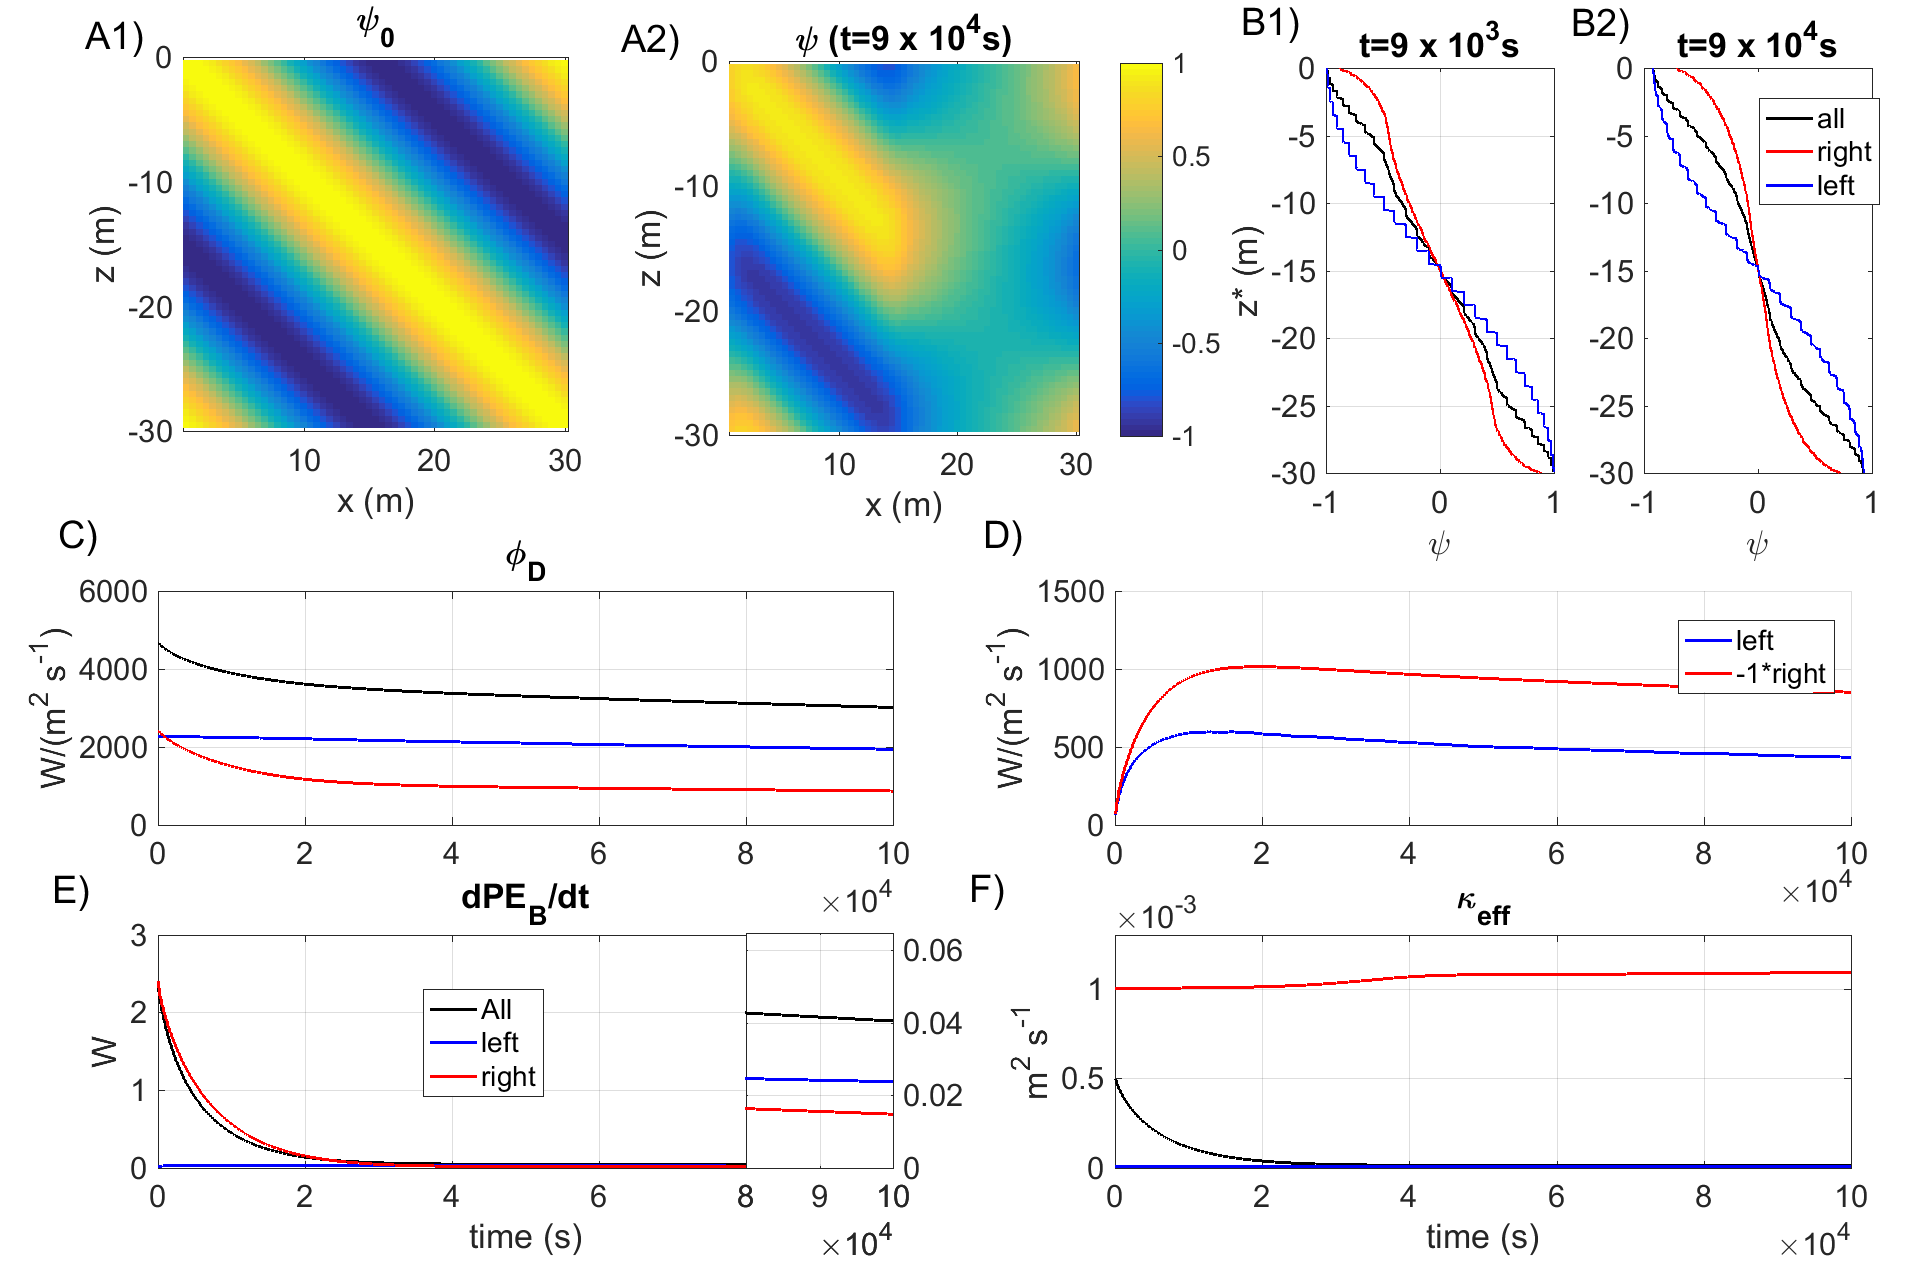
\includegraphics[width=1\textwidth]{./CHAP_BPE/AGBPE_numlab2_2.png}
\caption[Initial field and evaluation of $\kappa_{eff}$ for configuration $BPE_{exp}$]{(A1 and A2) Initial field of tracer $\psi$, and tracer field after $t=100s$ of simulation. (B1 and B2) Reference profiles $z^*(\psi)$ at $t=9.10^3s$ and $t=9.10^4s$ of simulation computed either with the fluid parcels of the left half sub-domain (blue), the right half sub-domain (red), or the complete domain (black). (C, D and E) RHS (C and D) and LHS (E) terms of equation \ref{bilanBPEal} computed on the different (sub-)domains. $F_D^{right}$ is indicated with a factor $-1$ in (D). (F) $\kappa_{eff}$ as evaluated in equation \ref{eq_kappaEff} with the previous terms on the different (sub-)domains.}
\label{fig2numlab}
\end{figure}
%Initial tracer field same as in fig \ref{fig1numlab}.
%\item Figure \ref{fig2numlab}. $dx=0.5$ m, $dz=0.5$ m, $L_x=30$ m, $L_z=20$ m, $dt=0.1s$. $\kappa_{exp}^x=\kappa_{exp}^z=\kappa_{exp}$ and $u=0$, no advection. RK3 timestepping scheme.
%\item For x$<$15 m, $\kappa_{exp} = 10^{-3}$, otherwise $\kappa_{exp} = 10^{-2}$ m$^2$/s.

The chosen initial passive tracer field is given by $\psi_2 (x,z)$ and is shown in figure (\noparref{fig2numlab}.A1).
To evaluate the capacity of the algorithm to deal with local variations of mixing (i.e. when the intensity of turbulent mixing is varying in space), the explicit diffusivity $\kappa_{exp}$ of equation \ref{eqAdvDiff} is non-homogeneous over the domain. It is two order of magnitude greater over the right half of the domain ($10^{-3}$ vs. $10^{-5} \ m^2/s$ in the left half), so that as can be seen in figure (\noparref{fig2numlab}.A2) gradients are smoothed faster in this part of the grid.

The evaluation of $\kappa_{eff}$ presented in the previous section is carried out either for each half domain or for the whole domain. Three $z^*(\rho)$ reference profiles (respectively $z^*_{left}$, $z^*_{right}$ and $z^*_{all}$) are consequently computed with the "re-arrangement" algorithm considering only the fluid parcels in the left sub-domain, the right sub-domain, or the whole domain. Examples of those profiles are presented in figures (\noparref{fig2numlab}.B1 and B2).

Figures (\noparref{fig2numlab}.C to F) present the terms of equation \ref{bilanBPEal} computed from the evolution of each reference profiles. It must be noted that neither the diffusive term $\phi_D$ nor the evolution of BPE $dPE_B/dt$ computed for the whole domain are equal to the sum of those terms computed on each half domain (for example $\phi_D^{all} \ne \phi_D^{left}+\phi_D^{right}$). This is due to the different definition of $z^*(\psi)$ depending on the domain extension chosen for the rearrangement. In the same way, the diffusive fluxes $F_D$ of figure (\noparref{fig2numlab}.D) do not cancel each other from one half domain to the other past the initialization as $z^*_{left}$ and $z^*_{right}$ diverge.
%In turn, the amplitude of the term $\phi_D$ varies depending if it is calculated for the latest $z^*_{all}$ reference profile or if it is obtained as the sum  $\phi_D^{left}+\phi_D^{right}$. The diapycnal fluxes $\phi_D^{left}$ and $\phi_D^{right}$ in this sum are themselves calculated respectively with the reference profiles $z^*_{left}$ or $z^*_{right}$. These fluxes do not cancel each other in so far as they are computed locally based on the local reference profiles of each sub-domain.

If the effective diffusivity $(\kappa_{eff})$ is evaluated over each half domain, figure (\noparref{fig2numlab}.E) shows that the algorithm provides the correct value of the diffusivity with: $\kappa_{eff}\approx\kappa_{exp}$, as the ratio of equation \ref{eq_kappaEff} is near constant. In contrast, if $\kappa_{eff}$ is now evaluated over the whole domain, it is initially equivalent to the overall explicit mean diffusivity $(\kappa_{left}+\kappa_{right})/2$ but it decreases afterwards with time, approaching the value of $\kappa_{exp}^{left}$ after $t \approx 3.10^4s$. So the global effective diffusivity is finally close to the smallest value in the domain. This smallest value is associated with the area of the domain in which gradients of the tracer field are at that time less affected by dissipation, with a slower evolution of $z^*$ as seen in figure (\noparref{fig2numlab}.B1 and B2).

%, as diffusion is 'more efficient' on the right half of the domain,
%Because $\kappa_{eff}$ is computed as homogeneous, it must reflect the global diffusion process, however as time goes by in the simulation, diffusion is more efficient over the right half domain, for greater and greater $t$ the gradients of $\psi$ there will be smoothed out before   NON This can be explained by the differences in the re-arranged reference profiles. When this reference profile is computed "locally" (this is the case when the effective diffusivity is evaluated locally to compute $\kappa_{right}$, it is smoothed out quicker. As a consequence, the evaluated diapycnal flux decreases.\color{black}
%As time goes on, the effective diffusivity 
%\color{red} $\kappa_{eff}$ tends to the lowest value of diffusivity since in the right half (left or right ?),
%the vertical gradient of $\psi$ will be deteriorated quicker, hence the term of the integrand is smaller and the higher value of the gradient of $\psi$ in the left half will... (je n'arrive pas à formuler : l'évolution pilotée par là où le coef est le plus bas une fois que les gradients à droite sont résorbés)
%\item only able to differentiate for $\kappa(x)$.
%If diffusion coefficient was made to vary along the vertical direction, in the same way that when evaluate $\kappa_{eff}$ for the whole domain, integrates all contributions to the change in $z^*$ in the water column
%Explique plus simplement en français... cette étude est un peu loin maintenant... Au pire, on le rédige ensemble lundi matin.


\subsection{Implicit diffusion case $(BPE_{imp})$}
A similar flow configuration is now investigated with homogeneous $\kappa_{exp}$ when advection is not neglected anymore ($u \ne 0$, table \ref{tab_NUMLAB_imp}).
\begin{table}[h]
        %\begin{minipage}{.6\textwidth}
        \centering
        \begin{tabular}{|c|c|c|}
                \hline
                Configuration $BPE_{imp}$ & \textit{Parameters}\\
                \hline 
                Numerical Model & Advection-diffusion equation of passive tracers\\
                $L_x$ & 30 m\\
                $L_z$ & 20 m\\
                $\Delta x$ & 0.5 m or 1.5 m\\
                $\Delta z$ & 0.5 m\\
                $\Delta t$ & 0.1 s\\
                Time stepping & RK3 \\
                Diffusivity & see text \\
                Advection & $U\ = 0.1\ m/s$ with UP1 or UP3 advective schemes.\\
                Initial field & With UP1 scheme: $\psi(x, z,\ 0)=\psi_2(x,z)$. \\
                 & With UP3 scheme: $\psi(x, z,\ 0)=\psi_1(x)$\\
                \hline
        \end{tabular}
        \captionof{table}{ $BPE_{imp}$ configuration: numerical parameters.}
        \label{tab_NUMLAB_imp}
        %\end{minipage}
\end{table}
%\item $dx=0.5$ m, $dz=0.5$ m, $L_x=30$ m, $L_z=20$ m, $dt=0.1s$ same as previously, but this time $U=0.1m/s$, and advection scheme either RK3-UP1 or RK3-UP3.
The objective with this new implementation is to evaluate the implicit diffusion $\kappa_{imp}$ due to upstream (UP1 or UP3) advective schemes. The effective diffusivity can be compared to the value obtained analytically for each upstream scheme. 

\subsubsection{First order upstream scheme (UP1)}
%Figure \ref{fig3numlab} shows the evolution of the implicit diffusivity obtained in the $BPE_{imp}$ configuration.
\begin{figure}[h!]
\centering
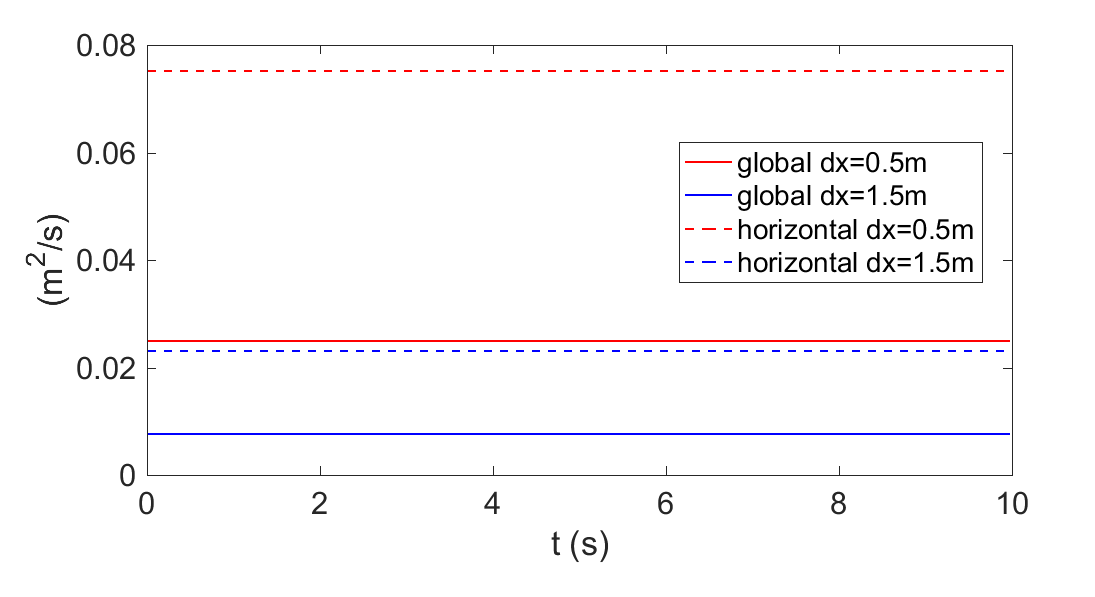
\includegraphics[width=0.5\textwidth]{./CHAP_BPE/AGBPE_numlab3.png}
\caption[Evaluation of $\kappa_{eff}$ for configuration $BPE_{imp}$ with RK3-UP1 scheme]{$\kappa_{eff}$ computed in the case of implicit diffusion with RK3-UP1 scheme for $\Delta x=0.5m$ (red) or $\Delta x=0.1m$ (blue). In the computation of $\kappa_{eff}$, either isotropic diffusion is assumed ($\kappa_v=\kappa_h$, lines) or that diffusion is only applied in the horizontal direction ($\kappa_v=0$, dashed lines)}
\label{fig3numlab}
\end{figure}
The initial field is the same as in the previous $BPE_{exp}$ configuration ($\psi_2(x,z)$, see figure (\noparref{fig2numlab}.A1)). Advective fluxes are now based on a first-order upstream scheme (UP1) and no explicit harmonic diffusion ($\kappa_{exp}=0$) is specified for now, so all diabatic evolution of $\psi$ will be due to the implicit effect of the advection scheme.
The modified equation for the discrete advection equation can be derived analytically:
\begin{equation}
\frac{\partial \psi}{\partial t}+U \frac{\partial \psi}{\partial x} = \frac{1}{2} U \Delta x  \frac{\partial^2 \psi}{\partial x^2} + \mathcal{O}(\frac{\partial^3 \psi}{\partial x^3})
\end{equation}
This leads to an analytical formulation of the implicit diffusion coefficient for the UP1 advective scheme: 
\begin{equation}
    \displaystyle
    \kappa_{h,imp}\approx\frac{1}{2}U \Delta x
\end{equation}
The implicit diffusivity consequently varies linearly with the grid scale and for $\Delta x\ =\ 0.5\ m$ (respectively $\Delta x\ =\ 1.5\ m$), it can reach $\kappa_{h,imp}\ =\ 0.025\ m^2/s$  (respectively $0.075\ m^2/s$).

Figure \ref{fig3numlab} shows that the correct value of the implicit diffusivity $(\kappa_{eff}=\kappa_{imp})$ can be recovered with the BPE algorithm only if the vertical component of the diffusion flux ($\phi_D$ in equation \ref{bilanBPEal}) is not taken into account, i.e. when only the along-flow diffusion flux is considered. If both the horizontal and vertical components of the fluxes are retained in the evolution equation, the BPE algorithm leads to a smaller value of the effective diffusivity.
%Otherwise, the simulated evolution of the tracer field is assumed to come from isotropic diffusion in both vertical and horizontal direction, consequently $\kappa_{eff}$ is evaluated as lesser since there is this added contribution of vertical diffusion of equation \ref{bilanBPEal}. Note that it is possible to know that this latter hypothesis is wrong only because the model is specified to have no explicit diffusivity and only horizontal advection that induces numerical diffusion along this direction. 


%the value of $\kappa_{eff}$ is less than the analytically-computed implicit diffusivity. In this later case, the effective diffusivity is indeed supposed to be applied to both the horizontal and vertical components of the flow in equation \ref{bilanBPEal}.

\subsubsection{Third order upstream scheme (UP3)}
In this third configuration, the initial tracer field is now $\psi(x,\ 0)=\psi_1(x)$ (see figure \noparref{fig5numlab}.A).% in such a way that the solution of advection-diffusion problem can be computed analytically: $\psi(x,t)=e^{-\kappa k_x^2 t}cos(k(x-Ut))$ with $k_x=2\pi/L_x$.
A third-order upstream advective scheme (UP3) is now associated to the RK3 time-stepping with a non-vanishing horizontal velocity. The modified equation leads this time to a 4th-order diffusion term:
\begin{equation}
\frac{\partial \psi}{\partial t}+U \frac{\partial \psi}{\partial x} = \underbrace{\frac{1}{120}(5 C^3-10) U \Delta x^3}_{k_4}  \frac{\partial^4 \psi}{\partial x^4} + \mathcal{O}(\frac{\partial^5 \psi}{\partial x^5})
\end{equation}
where $C\ =\ U\Delta t/\Delta x$ is the advection Courant number. With $C=2 . 10^{-2}$ in the present configuration, the fourth order diffusivity takes the value $k_4\ =\ -1.10^{-3} m^4/s$. Note that the BPE algorithm gives an implicit diffusion in form of a second-order diffusivity $k_2=\kappa_{eff}$.

This second-order effective diffusivity is evaluated for several experiments relying on this configuration (table \ref{table_kappa}). In those experiments, in addition to the effect of the implicit diffusivity from the $UP3$ scheme, explicit harmonic diffusion is added, so that the effective diffusivity should be the sum of both contributions $\kappa_{eff} \approx \kappa_{exp} + \kappa_{imp}$.
The computed effective diffusivity shows high-frequency oscillations with a non-negligible relative amplitude (not shown). Those oscillations are found regardless of the value of $\kappa_{exp}$. To filter out these oscillations, the value of $\kappa_{eff}$ indicated in table \ref{table_kappa} has been averaged over the whole simulation time. This is in agreement with the requirements of the treatment of the BPE evolution equation \ref{bilanBPEal} which requires that the effective diffusivity be computed over a period of time large enough with respect to the time-scale of the dissipation (see next section).
Once $\kappa_{exp}$ is removed from $\kappa_{eff}$, a unique value of $\kappa_{imp,2}$ is recovered at $4.65.10^{-5}\ m^2/s$ for all experiments.

\begin{figure}[h!]
\centering
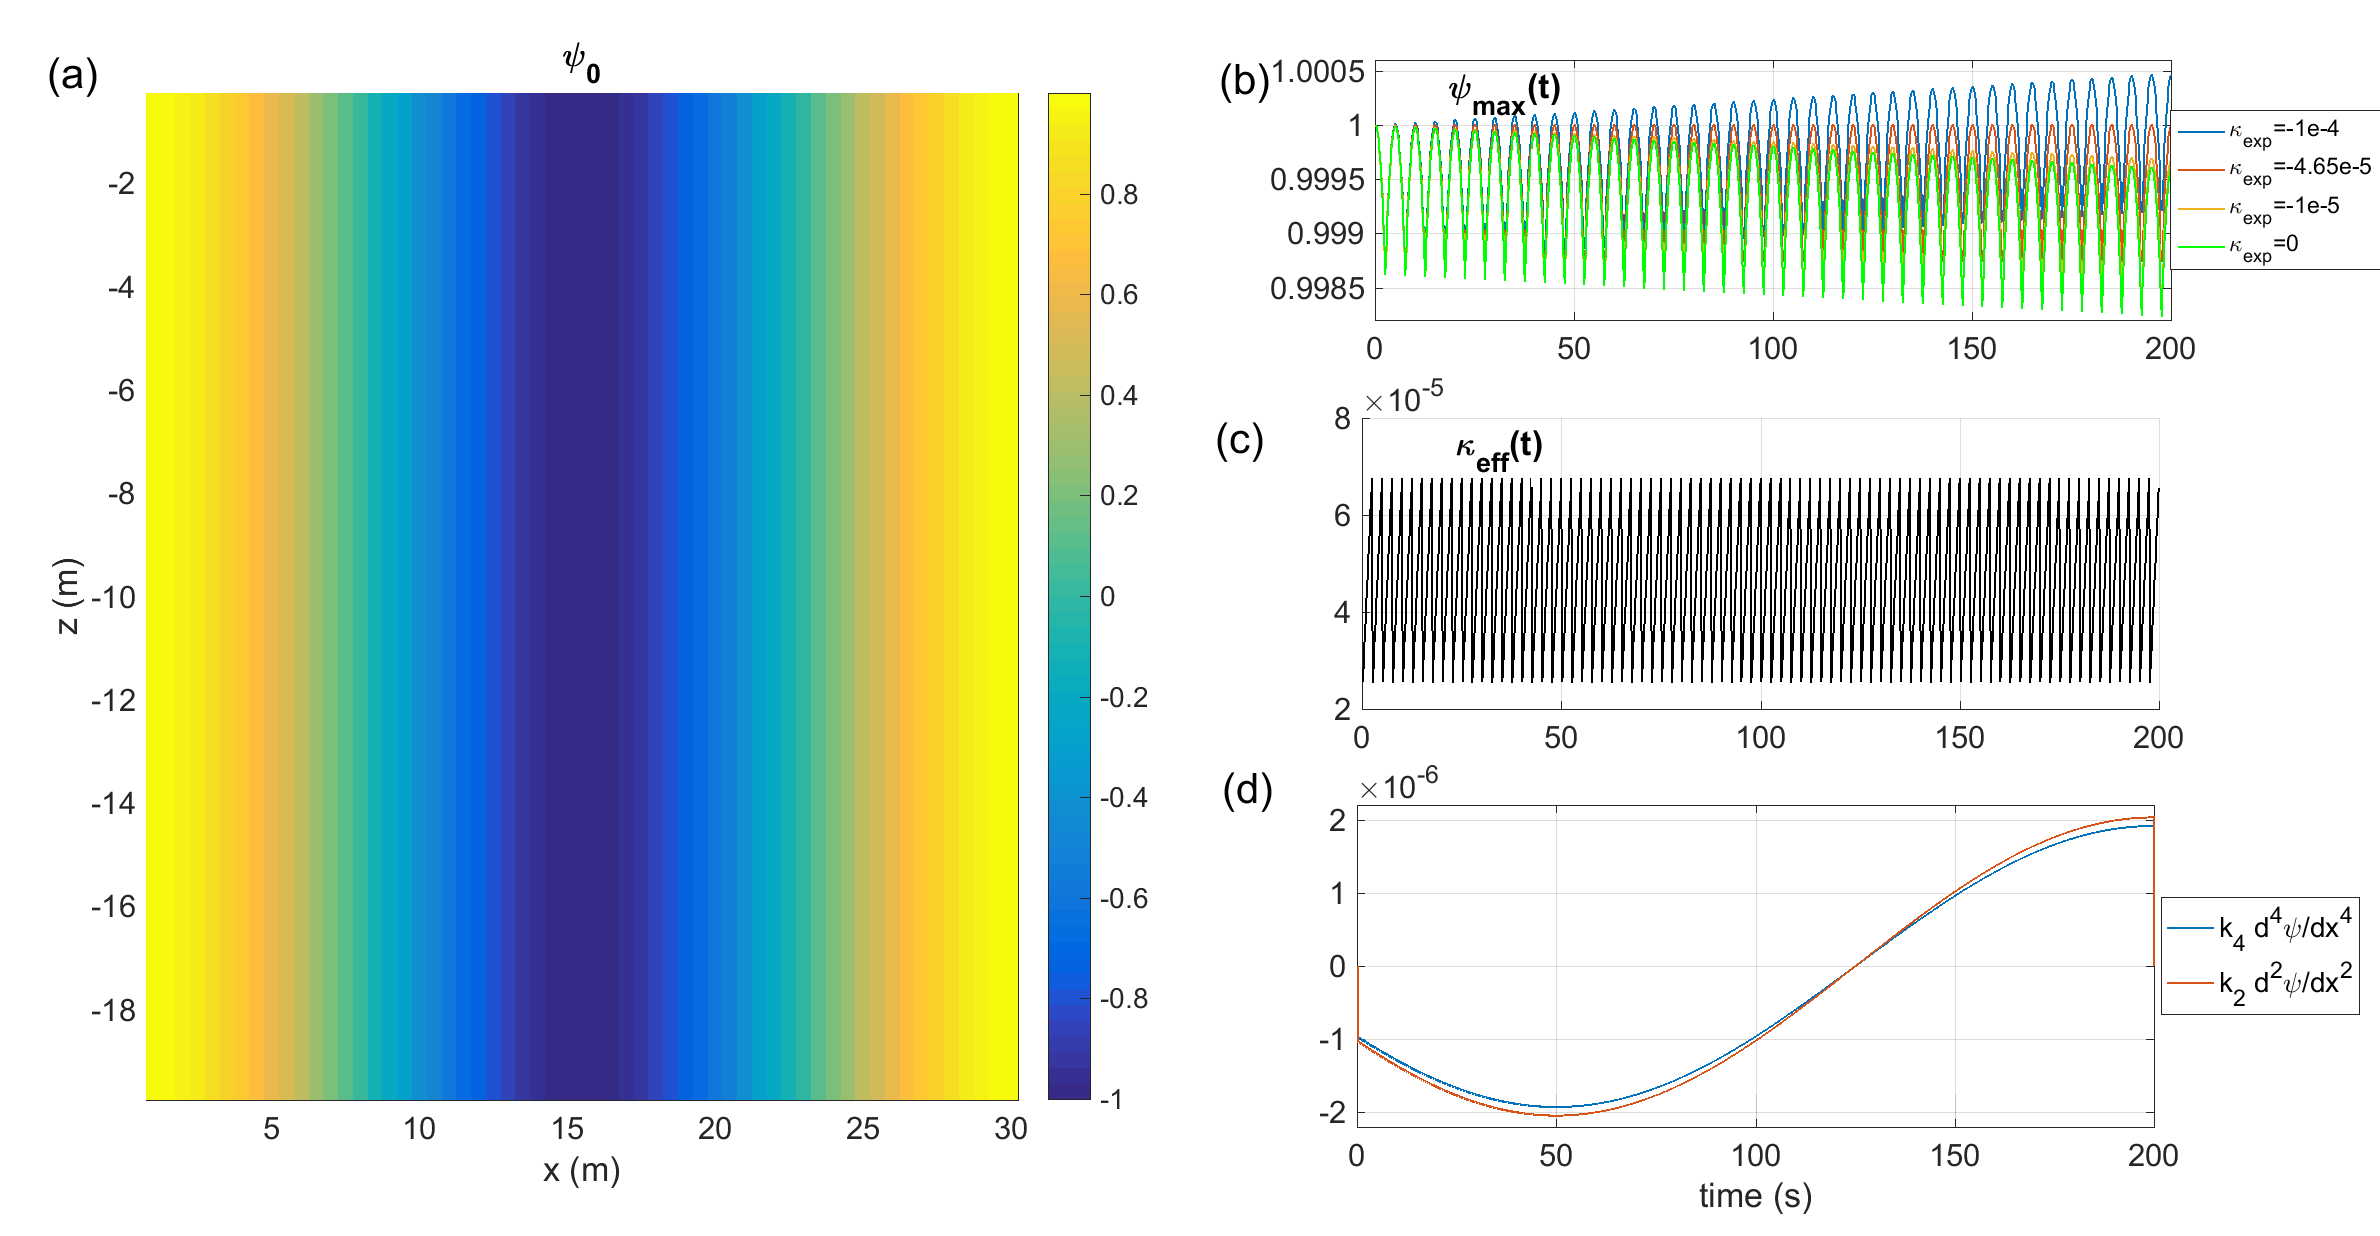
\includegraphics[width=1\textwidth]{./CHAP_BPE/AGBPE_numlab5.png}
\caption[Initial field and comparison of coefficient $k_2$ and $k_4$ for configuration $BPE_{imp}$ with RK3-UP3 scheme]{(A) Initial tracer field. (B) Comparison of the fourth-order (with analytical value of the coefficient $k_4$) and second-order (with value of $k_2$ deduced from $\kappa_{eff}$ in table \ref{table_kappa}) formulation of diffusion at a random grid point.}
\label{fig5numlab}
\end{figure}

%Several experiments are carried out with the configuration of schemes: in addition to the implicit diffusion induced by the upstream advection scheme, an explicit harmonic diffusion is also specified. 
%The effective coefficient found by BPE analysis consequently builds up to $\kappa_{eff} = \kappa_{exp} + \kappa_{imp}$.
%Figure \ref{fig5numlab}.b and table \ref{table_kappa} compare the effective diffusivity obtained with the BPE algorithm for several values of $\kappa_{exp}$. This diffusivity presents high-frequency oscillations with a non-negligible relative amplitude.
%\color{red}(correspond temps d'advection d'une cellule??? à vérifier (ou vient calcul des termes du bilan pas en RK3?))\color{black}. \\
%When averaged in time over the whole simulation, the effective diffusivity reaches approximately $4.65.10^{-5} m^2/s$ when $\kappa_{exp}\ =\ 0$. It is then evaluated for a series of configurations with non-zero explicit diffusivity and the (effective) implicit diffusivity $\kappa_{imp}$ is computed as the time-averaged effective diffusivity over the period minus the explicit diffusivity. The same  value of $4.65.10^{-5}\ m^2/s$ is recovered in all experiments.
%Since this value is for harmonic diffusion, the diffusion terms based on the effective second order diffusivity $(k_{imp,2}\ =\ \kappa_{eff}-\kappa_{exp})$ and on the analytical fourth-order diffusivity $k_4$ computed above can be compared in figure (\noparref{fig5numlab}.C) as factors of either the second or fourth order spatial derivate of $\psi$ taken at a random grid point. These terms are close to each other. 
To compare the effective second-order diffusivity $(k_{imp,2}\ =\ \kappa_{eff}-\kappa_{exp})$ with the analytical fourth-order diffusivity $k_4$, figure (\noparref{fig5numlab}.B) shows the evolution of the spatial serivate of the passive tracer field $(\psi)$ with the resulting second and fourth-order diffusion schemes. The resulting trends are close to each other.
Note however that the second-order and fourth-order advection terms do not operate in a similar way in wave-number space. Indeed, the fourth order is a more selective filter, smoothing more specifically small-scale gradients of passive tracer. This might be sufficient to explain the differences observed in figure (\noparref{fig5numlab}.B).
%\end{itemize}
\begin{table}[h!]
\centering
\begin{tabular}{|l|l|l|l|l|l|l|l|l|l|l|}
\hline
$\kappa_{exp}$ & $-10^{-4}$ &$-4.65.10^{-5}$ & $-10^{-5}$& $0$& $10^{-5}$& $10^{-4}$\\
\hline
$\kappa_{eff}$ & $-5.35.10^{-5}$ &$3.5.10^{-8}$ & $3.65.10^{-5}$& $4.65.10^{-5}$& $5.65.10^{-5}$& $14.65.10^{-5}$\\
\hline
$\kappa_{imp}$&\multicolumn{6}{c|}{$4.65.10^{-5}$}\\
\hline
\end{tabular}
\caption{Explicit diffusion coefficient ($\kappa_{exp}$) given to simulation, effective coefficient ($\kappa_{eff}$) computed from BPE analysis and implicit coefficient ($\kappa_{imp}$) by deducting one from the other (all in $m^2/s$)}
\label{table_kappa}
\end{table}

\subsection{Diffusion and advection timescales ($BPE_{ts}$)}
A third and last experiment ($BPE_{ts}$) based on the advection-diffusion equation \ref{eqAdvDiff} is now presented to better understand the limitation of the BPE algorithm in terms of characteristic time and length scales. The idea is that the BPE algorithm can only give an accurate, valuable value of the effective diffusivity if (i) this diffusivity can be considered as homogeneous and can thus be extracted from the integral of the diapycnal flux in equation \ref{bilanBPEal} and (ii) diapycnal fluxes can be evaluated over time-scales (much) larger than the time-scale of the diapycnal fluxes at stake but also larger than the remaining dynamical time-scales in the studied ocean region.
Table \ref{tab_NUMLAB_ts} oresents the physical and numerical parameters chosen for this experiment. The configuration is similar to $BPE_{exp}$ with the same distribution of $\kappa_{exp}$ but with active advection by a second-order centered scheme (C2) known to lead to a vanishing implicit dissipation.
\begin{table}[h]
        %\begin{minipage}{.6\textwidth}
        \centering
        \begin{tabular}{|c|c|c|}
                \hline
                Configuration $BPE_{ts}$ & \textit{Parameters}\\
                \hline 
                Numerical Model & Advection-diffusion equation of passive tracers\\
                $L_x$ & 30 m\\
                $L_z$ & 30 m\\
                $\Delta x$ & 0.5 m\\
                $\Delta z$ & 0.5 m\\
                $\Delta t$ & 10 s\\
                Time stepping & RK3 \\
                Diffusivity & Left: $\kappa_{exp} = 10^{-5} \ m^2/s$. Right: $\kappa_{exp} = 10^{-3} \ m^2/s$.\\
                Advection & $U_1\ = 2.10^{-4}\ m/s$, $U_2\ =\ 2.10^{-3}\ m/s$ with C2 advective scheme.\\
                Initial field & $\psi(x,\ 0)=\psi_1(x)$\\
                \hline
        \end{tabular}
        \captionof{table}{$BPE_{ts}$ configuration: numerical parameters.}
        \label{tab_NUMLAB_ts}
        %\end{minipage}
\end{table}

\begin{figure}[h!]
\centering
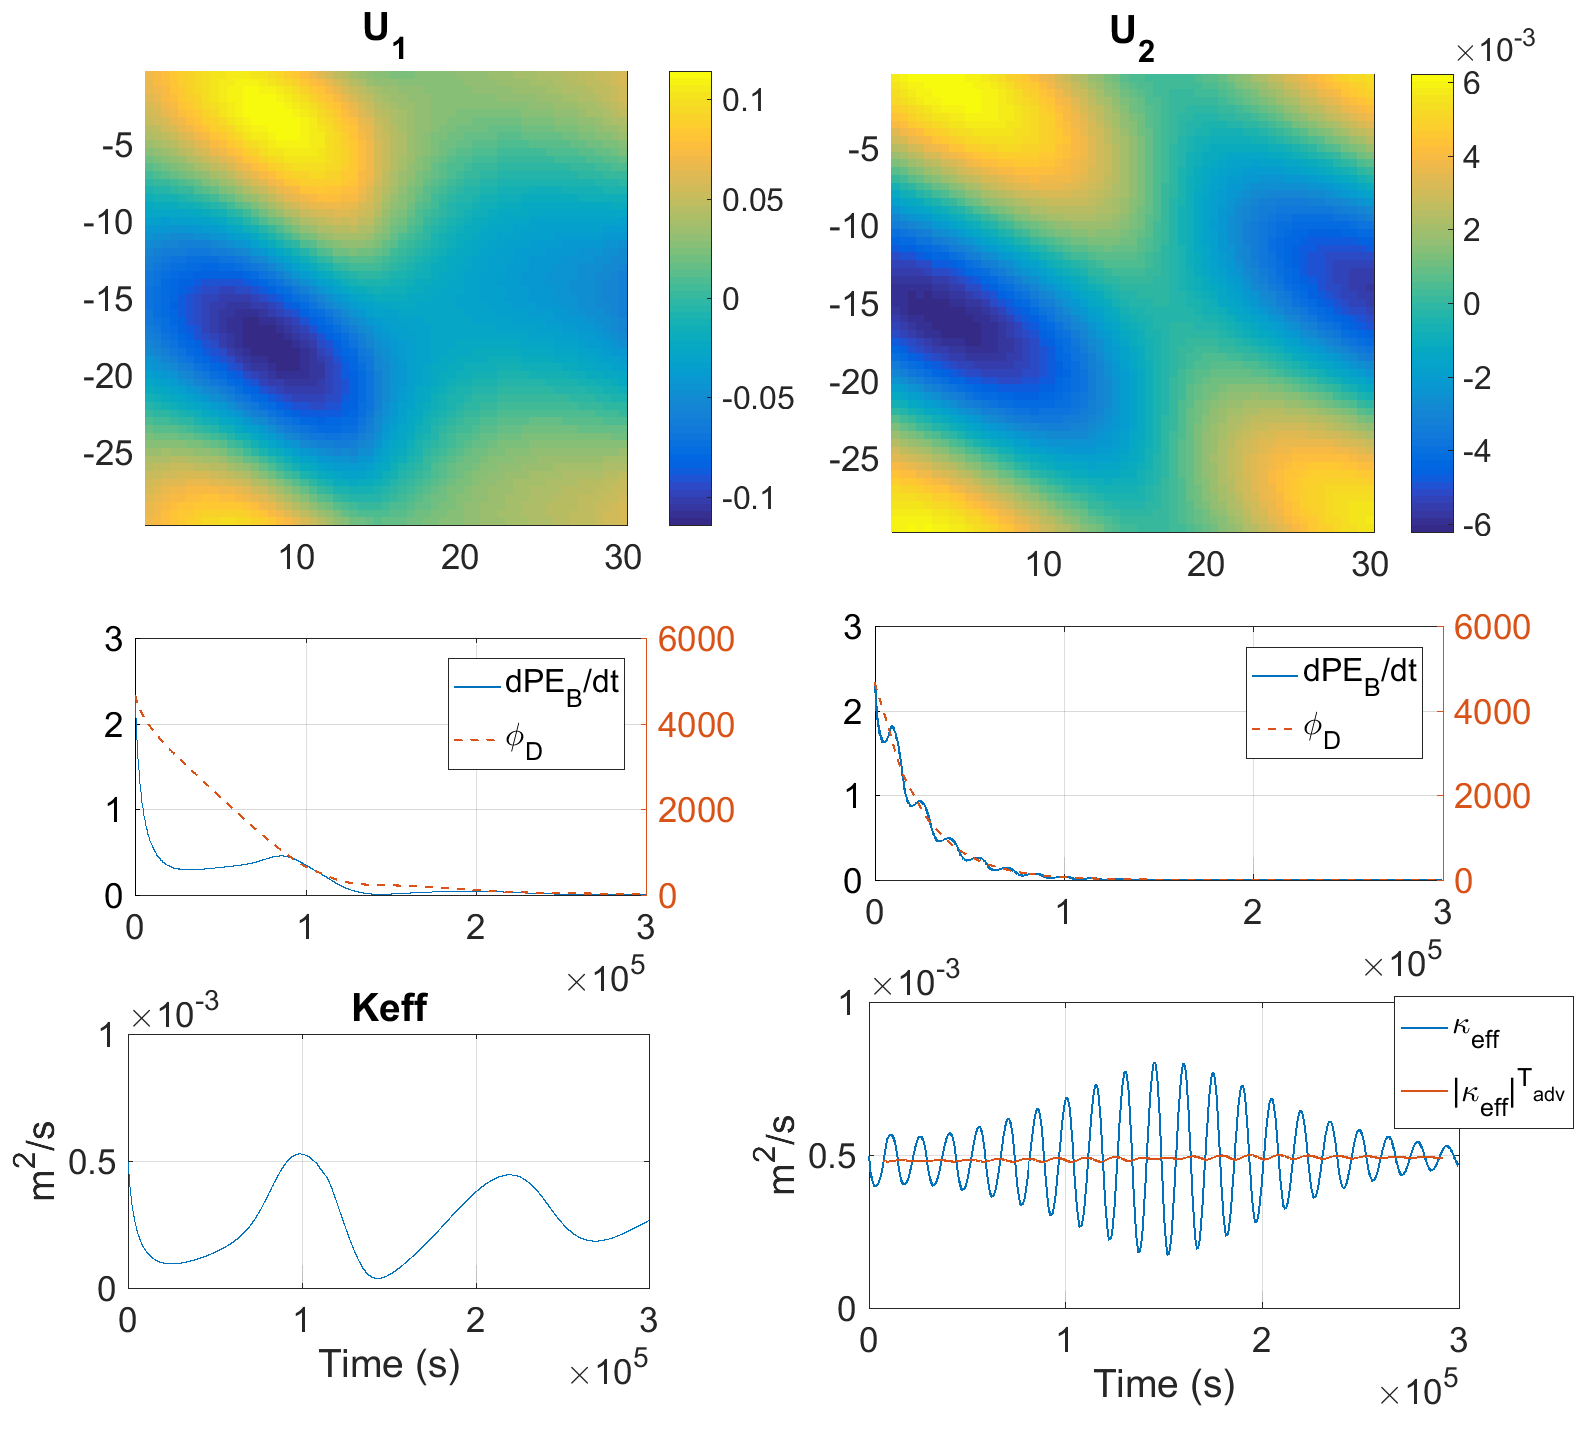
\includegraphics[width=1\textwidth]{./CHAP_BPE/Fig_numlab_advdiff3.png}
\caption[Tracer field and evaluation of $\kappa_{eff}$ for configuration $BPE_{ts}$]{(A1 and B1) Field of tracer $\psi$ at $t= \ 1.35\ 10^5\ s$ after initialisation for $u=2.10^{-4} \ m/s$ (A1) and $u=2.10^{-3} \ m/s$ (B1). (A2 and B2) Evolution of BPE (blue) and of term $\phi_D$ (red) of equation \ref{bilanBPEal} for each experiment. (A3 and B3) Value of instantaneaous $\kappa_{eff} (t)$ as computed in equation \ref{eq_kappaEff} (blue) for each experiment. In (B3) is also plotted in red the sliding averaged value of $\kappa_{eff}$ for a window $T_{adv}=T_{adv}^{U2}=1.5\ 10^4 s$.}
\label{fig4numlab}
\end{figure}
%\begin{itemize}
%\item RK3-C2 scheme (no implicit diffusion). $\Delta x = \Delta z = 0.5m$, $L = H = 30m$, $dt=10s$
%\item $\kappa(x)$ avec $\kappa = 10^{-5} \ m^2/s$ for left half of domain and $\kappa = 10^{-3} \ m^2/s$ for right half. 
%\item Horizontal advection, two cases, either $U_1=2 \ 10^{-4} m/s $ or $U_2=2 \ 10^{-3} m/s $
Characteristic timescales are evaluated for advection, $(T_{adv}=L_{adv}/U)$, and for diffusion $(T_{\kappa}=L_{\kappa}^2/{\kappa})$, where $L_i$ is the characteristic length-scale over which the flow is affected by each process. In this configuration, the explicit diffusion coefficient takes a different value in each half-domain so $L_{\kappa}\ =\ 15\ m$, whereas advection occurs with the same exact value over the whole domain so that $L_{adv}\ =\ 30\ m$. The value of advection however will change between two experiments.

This leads to the following time-scales : $T_{\kappa}^{left}=2.25 \ 10^7 \ s$, $T_{\kappa}^{right}=2.25 \ 10^5 \ s$, and (depending on the value of $U$) $T_{adv}^{U_1}=1.5 \ 10^5 \ s$ or $T_{adv}^{U_2}=1.5 \ 10^4 \ s$. As a consequence:
\begin{equation}
\displaystyle
T_{adv}^{U_2}<<T_{adv}^{U_1}<T_{\kappa}^{right}<<T_{\kappa}^{left}
\end{equation}

Figures (\noparref{fig4numlab}.A1 and B1) show the flow field after $t\ =\ 1.35\ 10^5 \ s$ for both values of the advective velocity. 

For the smallest advective velocity $U\ =\ U_1$ (figure A1), $t\ <\ T_{adv}^{U_1}$ and an advective cycle as not yet been completed.
%and the displacement of the structure remains small compared to the initial field. When $t$ approaches $T_{\kappa}^{right}$ the smoothing by the explicit dissipation is much larger over the left half domain.\\ 
For an advective velocity one order of magnitude greater $U\ =\ U_2$ (figure B1), $t\ >>\ T_{adv}^{U_2}$ and several advection cycles have happened, leading in the whole domain to smaller extremas of $\psi$ than in the $U=U_1$ case.
%and after several advection time-scales , the tracer field remains symmetric
%and the amplitude of the tracer-field variations are this time damped over the whole domain. This damping is higher than the damping induced by the smaller advective velocity field $(U_1)$ over the left part.

Figures (\noparref{fig4numlab}.A3 and B3) additionally show the variations with time of the effective diffusivity $\kappa_{eff}$ computed over the whole domain bor each case. 
%The average of the two values of explicit diffusivity prescribed over the whole domain is equal to $5 \ 10^{-4} \ m^2/s$.
With advective velocity $U_1$ (figure A3), the time-scales $T_{\kappa}^{right}$ and $T_{adv}^{U_1}$ are close, the effective diffusivity is initially close to the prescribed averaged explicit diffusivity $(5 \ 10^{-4} \ m^2/s)$ but quickly decreases. Figure (\noparref{fig4numlab}.A3) shows two oscillations of $\kappa_{eff}$ with a period of $\approx 1.2 \ 10^5s$, a minimum (maximum) value reached of $3.8 \ 10^{-5} \ m^2/s$ ($5 \ 10^{-4} \ m^2/s$). Those oscillations are not regular and seem to arrise from resonance between the advective and dissipative timescales $T_{adv}^{U_1}$ and $T_{\kappa}^{right}$, they do not average to the median value of diffusivity.
%. At $t\ =\ 2.785\ 10^5 s$, i.e. after approximately two advective time-scales $T_{adv}^{U_1}$, all the fluid parcels have been advected through the high dissipation area.
%As time goes on, this effective velocity shows oscillations over a period close to the advective time-scale. The effective diffusivity oscillates around a mean value twice as small as the average value of the prescribed explicit velocity. \\
%but after $t=3.86 \ 10^4 s$ , reach a minimum of $\kappa_{eff}=3.24 \ 10^{-5} m^2/s$. This value then increases again slowly then stabilizes at $\kappa_{eff}=2.2 \ 10^{-4} \ m^2/s$ after $t=2.785 \ 10^5 s$ approx half $T_{adv}^{U_1}$ at this point all original fluid parcels have been advected through the high dissipation area.
With a much larger advective velocity $U_2$ (figure B3) now, the effective diffusivity oscillates around the averaged explicit advective velocity. The time-scale of the oscillations is now smaller: it remains very close to the advective time-scale $T_{adv}^{U_2}$, with an enveloppe at a smaller frequency that could be linked to $T_{\kappa}^{right}$. When a sliding average operator with time window $T_{adv}^{U_1}$ is applied to the effective diffusivity most of the oscillations are cleared of the signal.

When the effective diffusivity is computed independently over each sub-domain, the expected prescribed values are recovered with smaller amplitude oscillations at the advective time-scale (not shown).
%and this diffusivity oscillates over the same advective time-scale but with a much smaller amplitude. 

\subsection{Partial conclusion}
The various experiments carried out in the frame of this simple but complete advection- diffusion configuration confirms that \cite{winters_available_1995}'s BPE algorithm can lead to a quantification but also to a localization of the turbulent mixing coefficient in regional ocean configurations. This includes an evaluation of the implicit dissipation induced by advective schemes.
%It has also been confirmed that this algorithm can conveniently be used to evaluate the implicit dissipation induced by advective schemes.
%Large variations of the effective diffusivity can yet be observed when it is evaluated over a period smaller than or close to time-scales of active process (such as the advective time-scale in the proposed experiments). To be accurate, this effective diffusivity must in any event be carried out over time-scale larger than the estimated time-scale of the diapycnal fluxes in the region of interest. 
Quantification is achieved through the determination of an effective diffusivity, to be
viewed as an average for the region (viewed as a sum of water-columns) over which the evolution equation \ref{bilanBPEal} has been evaluated. However, in this advection- diffusion configuration, advection through areas of localized diffusion leads to oscillations of the evaluated effective diffusivity at the advection time-scale. 

%large variations of the effective diffusivity 

%%%%%%%%%%%%%%%%%%%%%%%%%%%%%%%%%%%%%%%%%%%%%%%%%%%%%%%%%%%%%%%%%
\section{Toward an evaluation of mixing in real ocean}
%%%%%%%%%%%%%%%%%%%%%%%%%%%%%%%%%%%%%%%%%%%%%%%%%%%%%%%%%%%%%%%%%
\label{section_CROCO_BPE}
Several additional test configurations of increasing complexity are now presented to progress toward an evaluation of mixing in a "real ocean" with the "generalized" BPE algorithm presented in \S \ref{BPE_algo}. The consequences of the variations of the ocean free-surface are thus first explored in the case of the free oscillations of a stratified tank. Mixing is then finally evaluated with the BPE algorithm when Kelvin-Helmholtz instabilities are developing and in the region of Gibraltar strait.

\subsection{Free oscillations of a stratified tank}
\subsubsection{Linear stratification and free surface: induced mixing ($BPE_{tank}$)}

As shown in \S \ref{section_PE_chap2}, the variations of the ocean free-surface induce several adaptations of the evolution equation of BPE and, as a consequence, they have a significant impact on the evaluation of mixing in realistic configurations. The present configuration focuses on the mixing of a stratified fluid induced by the natural (free) oscillations of a stratified tank initially subjected to a gradient of free-surface anomaly. The physical and numerical parameters are presented in table \ref{tab_BPE_TANK}.

\begin{table}[h]
        %\begin{minipage}{.6\textwidth}
        \centering
        \begin{tabular}{|c|c|c|}
                \hline
                Configuration $BPE_{tank}$ & \textit{Parameters}\\
                \hline 
                Numerical Model & CROCO (compressible, non-hydrostatic kernel)\\
                $L_x$ & 50 m\\
                $L_z$ & 10 m\\
                $\Delta x$ & 0.2 m\\
                $\Delta z$ & $\approx\ 0.2\ m$\\
                $\Delta t$ & close to CFL requirements in test-configurations\\
                Diffusivity & $\kappa_{exp} = 4.10^{-6} \ m^2/s$\\
                \hline
        \end{tabular}
        \captionof{table}{$BPE_{ts}$ configuration: numerical parameters.}
        \label{tab_BPE_TANK}
        %\end{minipage}
\end{table}
The initial perturbation of the ocean free-surface is chosen equal to:
\begin{equation}
\displaystyle
\zeta(x,t=0)=\zeta_0\ cos\left(\frac{\pi x}{L_x}\right)
\end{equation}
with $\zeta_0\ =\ 2\ mm$.
%Now apply determination of $\kappa_{eff}$ to numerical cases Based on TANK experiment (ref?), adapted to have stratification. Evolution of the density tracer field, through the complete system of equation for ocean CROCO. Closed domain, 2D. No initial velocity.

The initial anomaly of the free-surface induces natural oscillations of the linearly stratified flow presented in figure (\noparref{figClin}.A) due to the propagation and resonance of surface gravity waves. The induced currents are expected to lead to diapycnal fluxes and, as a consequence, participate to increase turbulent mixing.

\begin{figure}[h!]
\centering
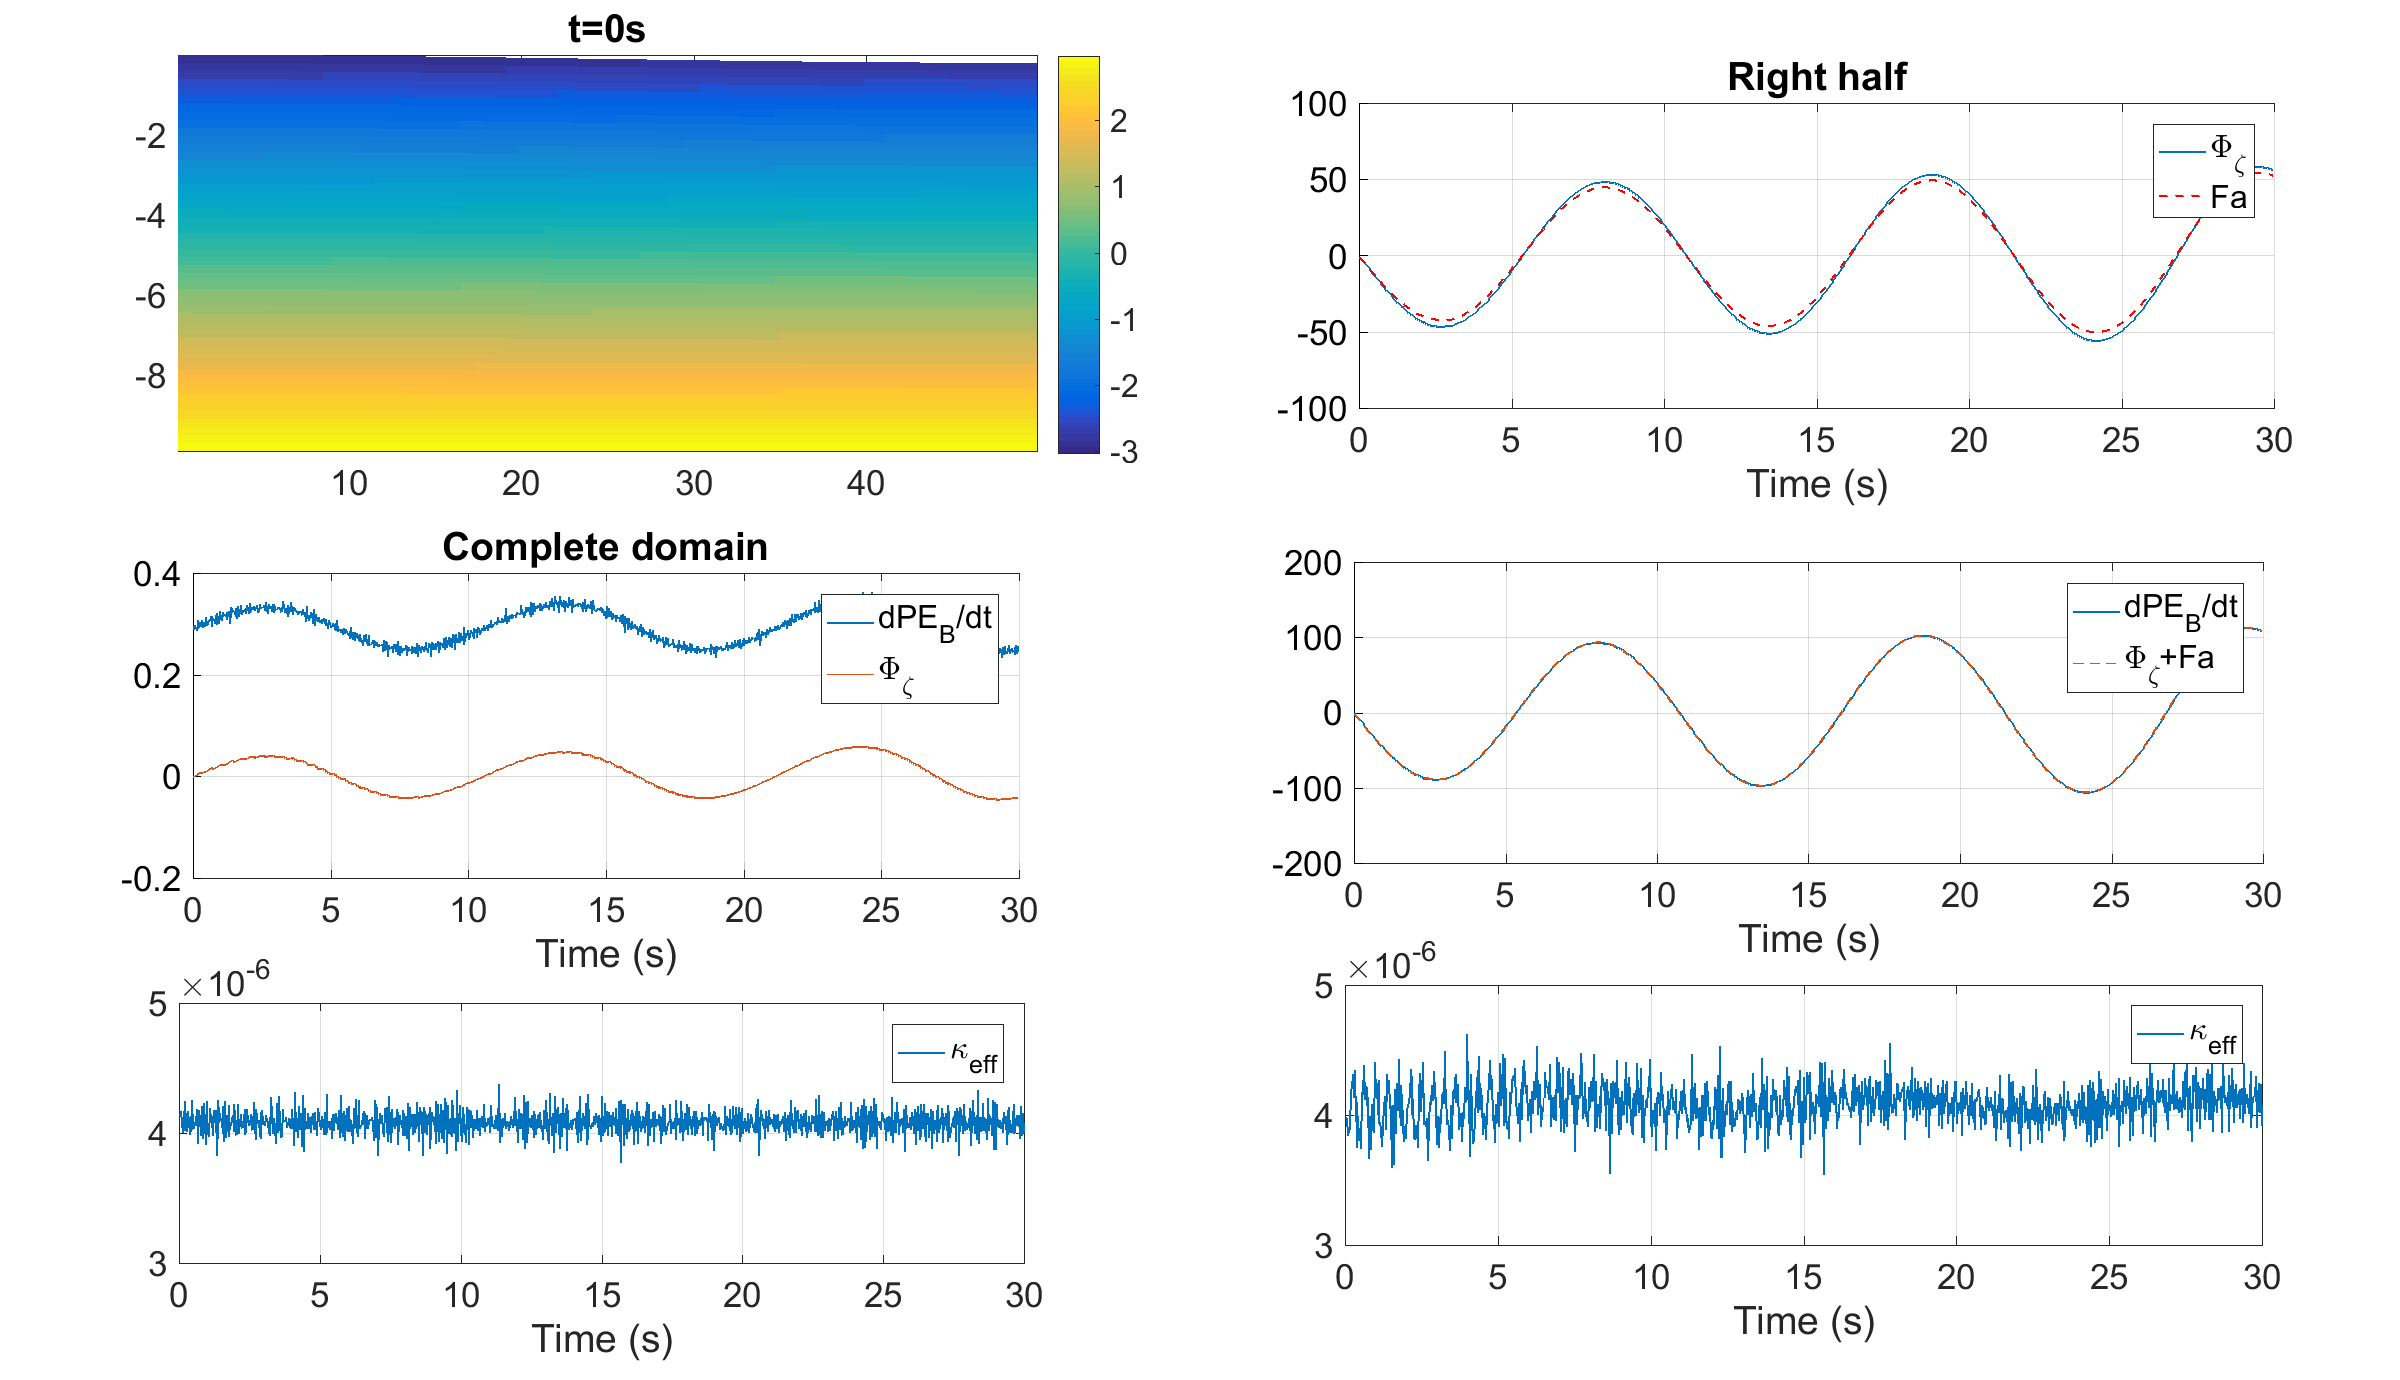
\includegraphics[width=1\textwidth]{./CHAP_BPE/Fig_TANK_linS.png}
\caption[Initial tracer field and evaluation of $\kappa_{eff}$ for configuration $BPE_{tank}$]{(A) Initial tracer field of the $BPE_{tank}$ configuration. (B1 and B2) Evaluation of the time evolution of some terms of the balance equation \ref{bilanBPEal} over the whole simulated domain. (C1 to C3) same as B1 and B2 but for an evaluation carried out only on the right half of the domain.}
\label{figClin}
\end{figure}
%Movement comes from evolution of initially non-flat free surface. Initial linear stratification $\rho(z)$ (ie, constant N) see figure (\noparref{figClin}.A). $\rho_0=1043 kg/m^3$
%\item L$=$50m, H$=$10m, dx$=$0.2m$\approx$dz, amplitude oscillation initiale de la surface libre de 2mm. Explicit diffusion coefficient put at $10^{-4}$m$^2$/s. 
Figure (\noparref{figClin}.B1-B2 and C1 to C3) show %the initial density field together with 
the evolution with time of the various terms in the balance equation \ref{bilanBPEal}. Computations are successively carried out for the whole domain (figures (\noparref{figClin}.B1 and B2)) or for the right half domain (figures (\noparref{figClin}.C1 to C3)).

As could be expected, the oscillations of the free-surface clearly governs not only the variations of the first term $(\phi_{\zeta})$ of this balance equation but also the variations of the overall BPE variations $(dPE_B/dt)$. Indeed, the long-wave phase speed of surface gravity waves $(c\ =\ \sqrt(g L_z)\approx\ 9.9\ m/s)$ induces a natural time-scale of oscillations of the tank of $T_{\zeta}\ =\ L_x/c\ =\ 5\ s$ when freely propagating from a wall to the other. The period of the oscillations of $dPE_b/dt$ and $\phi_{\zeta}$ are close to twice $T_{\zeta}$.

If the balance equation is evaluated over the whole domain (left column of figure \ref{figClin}), the free-surface term of the evolution equation explains the oscillations of $(dPE_B/dt)$ (figure \noparref{figClin}.B1) and the prescribed explicit diffusivity is recovered with good accuracy (figure \noparref{figClin}.B2) with only some spurrious small amplitude noise.

If the balance equation is now evaluated over the right half domain only (figures \ref{figClin}.C1 to C3), $\phi_{\zeta}$ is approximately equal to $F_a$ the sum of the advective flux of BPE through the (vertical) lateral boundary of this sub-domain (figure \noparref{figClin}.C1). Note that the terms of the evolution equation are all several orders of magnitude larger than when the balance equation is evaluated over the whole domain. The effective diffusivity is still recovered with good accuracy (figure \noparref{figClin}.C3).

These results confirm the pertinence of the proposed BPE balance equation \ref{bilanBPEal} and reinforce the choices made to evaluate numerically the BPE algorithm. Even in a case where the induced mixing is several order of magnitudes smaller than the other terms of the balance equation, the explicit diffusivity can therefore be recovered both globally and locally based on \ref{eq_kappaEff}, provided that the term $\phi_{\zeta}$ is taken into account.
%If make computation on a half domain $\Phi_{\zeta}$ is of the same amplitude as $F_a$ the advective fluxes. All terms are bigger.
%\item find $\kappa_{eff}$ of the explicit value that was given. Without taking into account $\Phi_{\zeta}$ would have leftover oscillations.

\subsubsection{Pycnocline and free surface ({$BPE_{tank2}$})}
The mixing induced by the natural oscillations of tank are now explored for a two-layer stratification (i.e. for a sharp ocean pycnocline). Most parameters of table \ref{tab_BPE_TANK} remain unchanged except for the prescribed diffusivity now put at $10^{-4}m^2/s$.

%\begin{table}[h]
%        %\begin{minipage}{.6\textwidth}
%        \centering
%        \begin{tabular}{|c|c|c|}
%                \hline
%                Configuration $BPE_{tank2}$ & \textit{Parameters}\\
%                \hline 
%                Numerical Model & CROCO (compressible, non-hydrostatic kernel)\\
%                $L_x$ & 50 m\\
%                $L_z$ & 10 m\\
%                $\Delta x$ & 0.2 m\\
%                $\Delta z$ & $\approx\ 0.2\ m$\\
%                $\Delta t$ & Close to CFL requirements in test-configurations.\\
                %Diffusivity & $\kappa_{exp} = 10^{-4} \ m^2/s$\\
%                \hline
%        \end{tabular}
%        \captionof{table}{$BPE_{ts2}$ configuration: numerical parameters.}
%        \label{tab_BPE_TANK2}
%        %\end{minipage}
%\end{table}
\begin{figure}[h!]
\centering
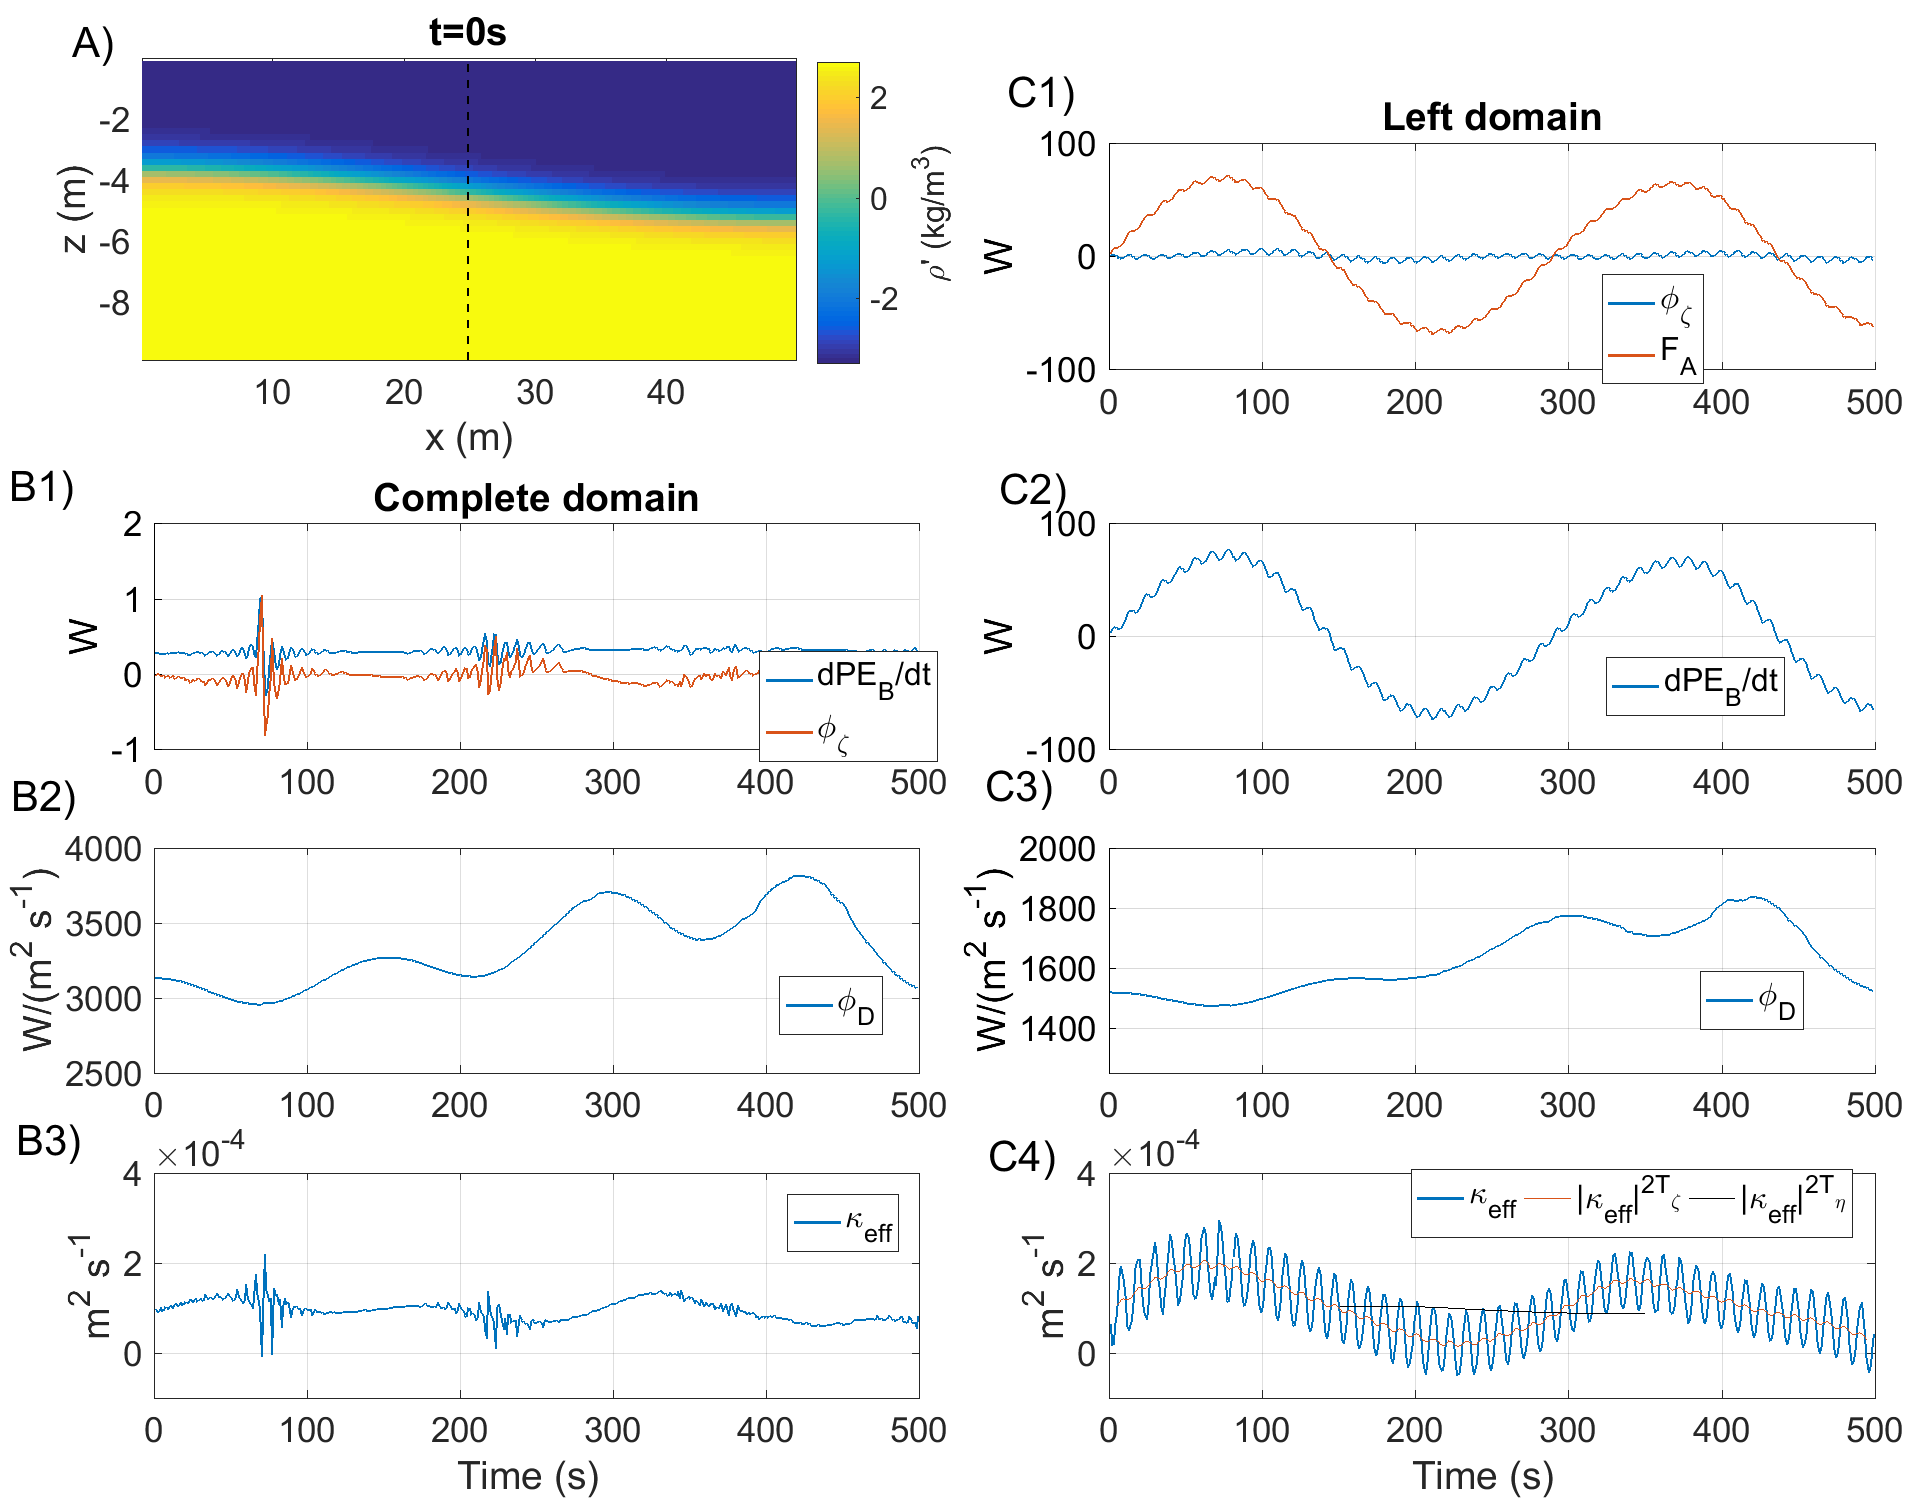
\includegraphics[width=1\textwidth]{./CHAP_BPE/Fig_TANK_pyc.png}
\caption[Initial tracer field and evaluation of $\kappa_{eff}$ for configuration $BPE_{tank2}$]{(A) Initial tracer field of the $BPE_{tank2}$ configuration. (B1 to B3) Evaluation of the time evolution of some terms of the balance equation \ref{bilanBPEal} over the whole simulated domain. (C1 to C4) Same but for an evaluation carried out only on the left half of the domain.}
\label{figCpsin}
\end{figure}
Two types of "interfacial" gravity waves can now propagate in this stratified tank: a surface gravity wave with a phase speed of $\sqrt(g L_z) \ \approx \ 9.9\ m/s$ and an internal gravity wave with an interfacial wave speed of $\sqrt(g' h_1 (L_z-h_1)/L_z\ =\ 0.33\ m/s$ ($h_1$ being the depth of the pycnocline). The corresponding time-scales are $T_{\zeta} \ = \ 5 \ s$ and $T_{\eta} \ = \ 150 \ s$.
%\item dx$=$dz$=$0.2m, L$=$50m, H$=$10m. Explicit coefficient put at $10^{-4}$m$^2$/s. \color{red}$\rho_0=$\color{black}
%\item Speed surface waves $\sqrt(gH)=5m/s ?????$ and $T_{\zeta}=5s$
%interfacial wave $\sqrt(g'h_1h_2/H)=0.33m/s$ and $T_{\eta}=150s$

The free-surface is supposed to be initially at rest whereas the sinusoidal-shaped initial stratification is shown in figure (\noparref{figCpsin}.A).

As with the previous configuration the evolution of the terms of the balance equation \ref{bilanBPEal} are first evaluated over the whole domain in figures (\noparref{figCspin}.B1 to B3), then over one half in figures (\noparref{figCspin}.C1 to C4).

The evaluation of $\kappa_{eff}$ carried out on the entire domain (figure (\noparref{figCpsin}.B3)) is close to the prescribed diffusivity with a regular pattern of noise (first at $t\ =\ 80\ s$), that could come from interaction of the pycnocline with the boundaries of the closed domain.

In the left half domain, $F_A>>\phi_{\zeta}$ (figure (\noparref{figCpsin}.C1)) in contrast to the previous case, with the evolution in the trend of BPE (figure (\noparref{figCpsin}.C2)) mainly explained by the advective flux. The term $\phi_{\zeta}$ still retains a non-negligible part of the high-frequency variability. The evolution of $\kappa_{eff}$ in this half domain now clearly shows two oscillations frequency, as shown in figure (\noparref{figCpsin}.C3), corresponding to $2T_{\zeta}$ and $2T_{\eta}$. When the signal is averaged over this latter period, the prescribed diffusivity is found again. The diffusivity $\kappa_{eff}$ evaluated on the right domain (not shown) as an evolution symmetric relative to this average to the one in the left domain.


%If the high-frequency oscillations due to the free-surface contribution are filtered out, an increase (decrease) in BPE can be observed in each half domain when the depth of the interface increases (decreases).
%, and respectively BPE will decrease as the interface gets shallower.
%Figure \ref{figCpsin} also shows that time-scales associated with the free-surface oscillations do not show up when BPE calculations are carried out over the whole domain but only if they are restricted to half domains. At the opposite, the internal interfacial oscillations can be observed on both type of computations: several pick can even be observed (first at $t\ =\ 80\ s$).
%Otherwise timescale associated with the interface for half domain and also for all the domain. See for all domain a signal (pics a $t=80s$)
%\item note that oscillations in half domain can sometime give a $\kappa_{eff}$ of negative value ( à expliquer... car le prend homogene et isotrope?)
%Figure \ref{figCpsin}.c shows the evolution in time of the effective diffusivity when BPE computations are successively carried out over the whole domain (red curve) or over half domains (blue curves). The latter curves present larger-amplitude oscillations but all curves oscillate around the value of the prescribed explicit velocity.

\subsubsection{Pycnocline, free surface and bottom bathymetry ($BPE_{tank3}$)}
The last experiment carried out for the tank configuration includes variations of the bathymetry. The objective is to evaluate the limitations of the BPE algorithm for in non-flat domains. The physical and numerical parameters are the same as those given in table \ref{tab_BPE_TANK} except for the depth $L_z$ which now varies linearly between 10 to 9.25 m, the width $L_x$ is now 10 m, and the prescribed diffusivity is $10^{-4}m^2/s$ as in the $BPE_{tank2}$ configuration. 

\begin{figure}[h!]
%\begin{subfigure}{.5\textwidth}
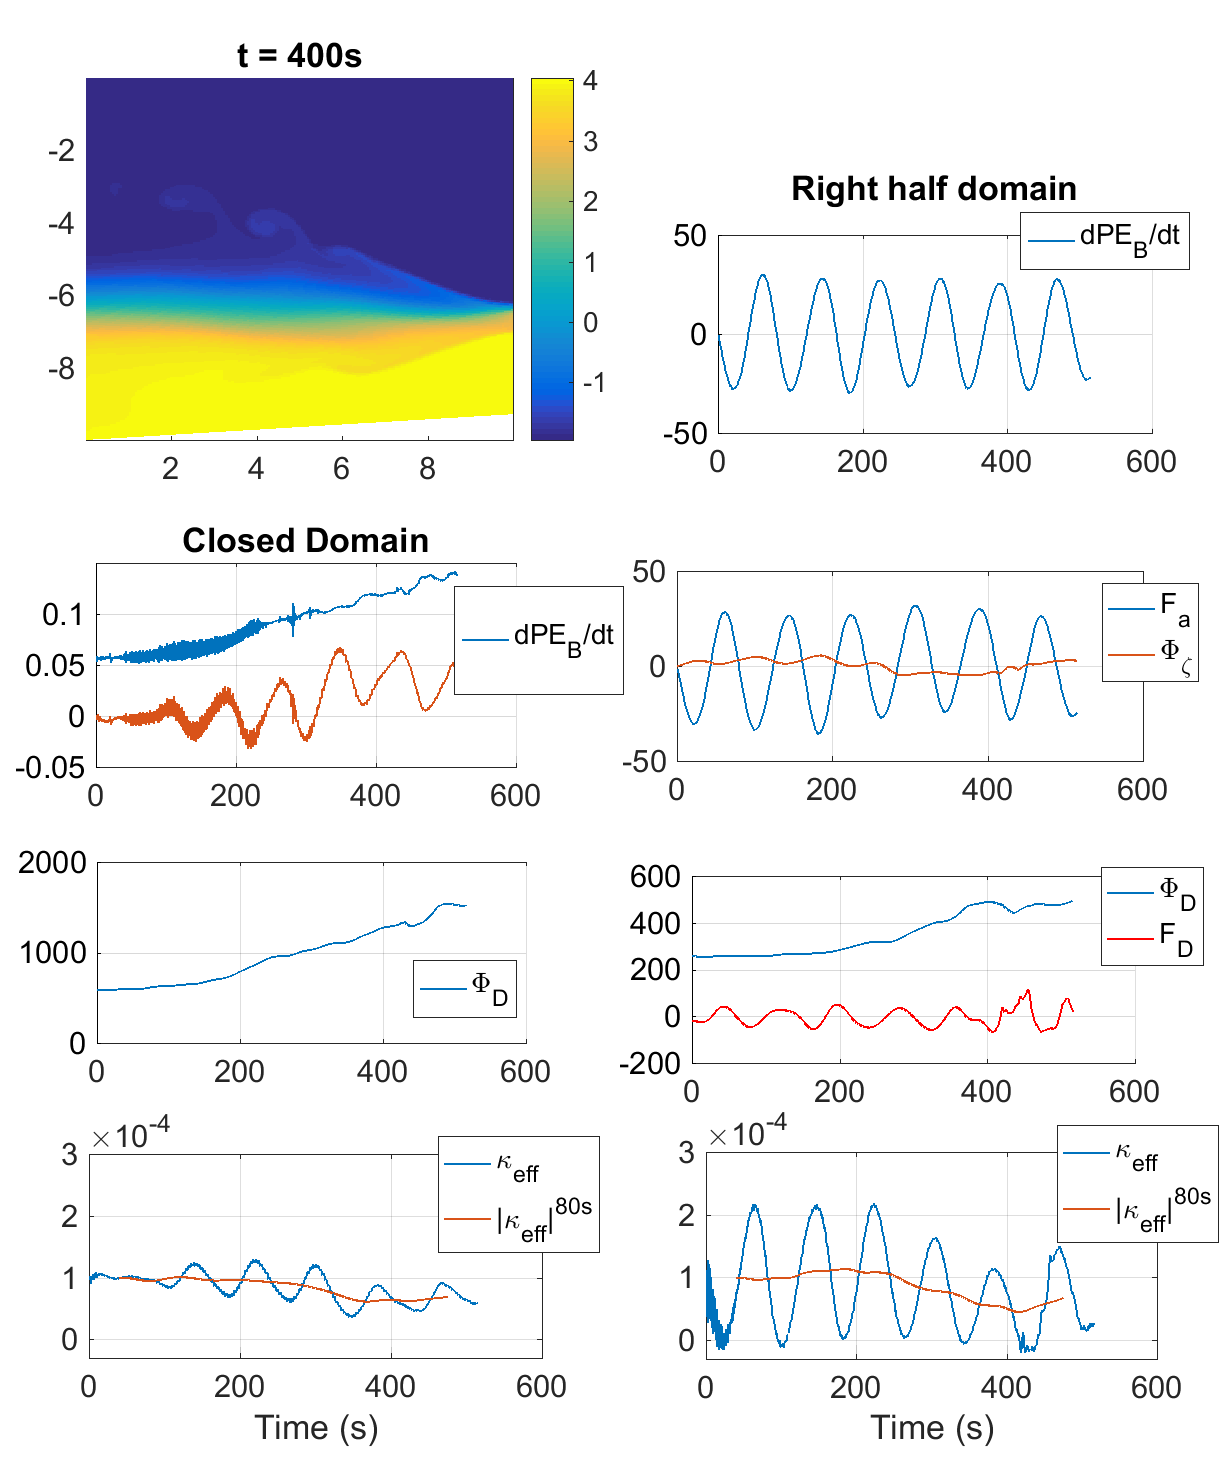
\includegraphics[width=1.\textwidth]{./CHAP_BPE/Fig_TANK_pycbath.png}
%\caption{Closed domain}
%\label{figCkh}
%\end{subfigure}
\caption[Initial tracer field and evaluation of $\kappa_{eff}$ for configuration $BPE_{tank3}$]{(A) Initial tracer field of the $BPE_{tank3}$ configuration. (B1 to B3) Evaluation of the time evolution of some terms of the balance equation \ref{bilanBPEal} over the whole simulated domain. (C1 to C4) Same but for an evaluation carried out only on the left half of the domain.}
\label{figCbath}
\end{figure}
%\item dx$=$dz$=$0.05m (200 vertical levels), L$=$10m, H$=$10m to 9.25m.$\rho_0=1042 kg/m^3$ Explicit coefficient put at $10^{-4}$m$^2$/s.
%\item Speed of surface waves $\approx 5m/s$,$T_{\zeta}=2s$
%The interfacial internal wave velocity is about $30\ s$.\\ 
The phase speed of internal, interfacial waves is in this case approximately equal to $0.32\ m/s$ and the corresponding time-scale is approximately $T_{\eta}\ =\ 30\ s$.

In this configuration, the initial slope of the pycnocline leads to Kelvin-Helmholtz instabilities after approximately 6 mn.\\
The BPE evolution equation evaluated over the whole domain shows an increase the variations of both $dPE_B/dt$ and $\phi_D$. The term associated to the free-surface oscillations $(\phi_{\zeta})$ is shown to oscillate at a period of $80\ s$ which does not correspond to the expected timescale of free-surface oscillations. The same type of oscillations can be observed on the variations of $\kappa_{eff}$. 
The BPE balance equation is evaluated over the right half domain in figure \ref{figCbath} (but a symmetric behaviour can be found for the left half). The advective flux term $(F_a)$ shows larger amplitude oscillations than $\Phi_{\zeta}$ but those oscillations have the same time-scale $(80\ s)$ as the BPE evolution.
%\end{itemize}

%%%%%%%%%%%%%%%%%%%%%%%%%%%%%%%%%%%%%%%%%%%%%
\subsection{Kelvin-Helmholtz Instability ($BPE_{kh}$)}
%\subsubsection{Kelvin-Helmholtz Instability : local estimation and mixing event}
The following configuration focuses on the large turbulent eddies associated to Kelvin-Helmholtz instabilities based on a previous study by \citet{penney_diapycnal_2019}. The corresponding physical and numerical parameters are given in table \ref{tab_BPE_KH}.
\begin{table}[h]
        %\begin{minipage}{.6\textwidth}
        \centering
        \begin{tabular}{|c|c|c|}
                \hline
                Configuration $BPE_{kh}$ & \textit{Parameters}\\
                \hline 
                Numerical Model & CROCO (compressible, non-hydrostatic kernel)\\
                $L_x$ & 256 m\\
                $L_z$ & 256 m\\
                $\Delta x$ & 2 m\\
                $\Delta z$ & $\approx\ 2\ m$\\
                Boundary conditions & Cyclic\\
                $\Delta t$ & Close to CFL requirements in test-configurations.\\
                Diffusivity & $\kappa_{exp} = 10^{-4} \ m^2/s$\\
                \hline
        \end{tabular}
        \captionof{table}{$BPE_{kh}$ configuration: numerical parameters.}
        \label{tab_BPE_KH}
        %\end{minipage}
\end{table}
\begin{figure}[h!]
\centering
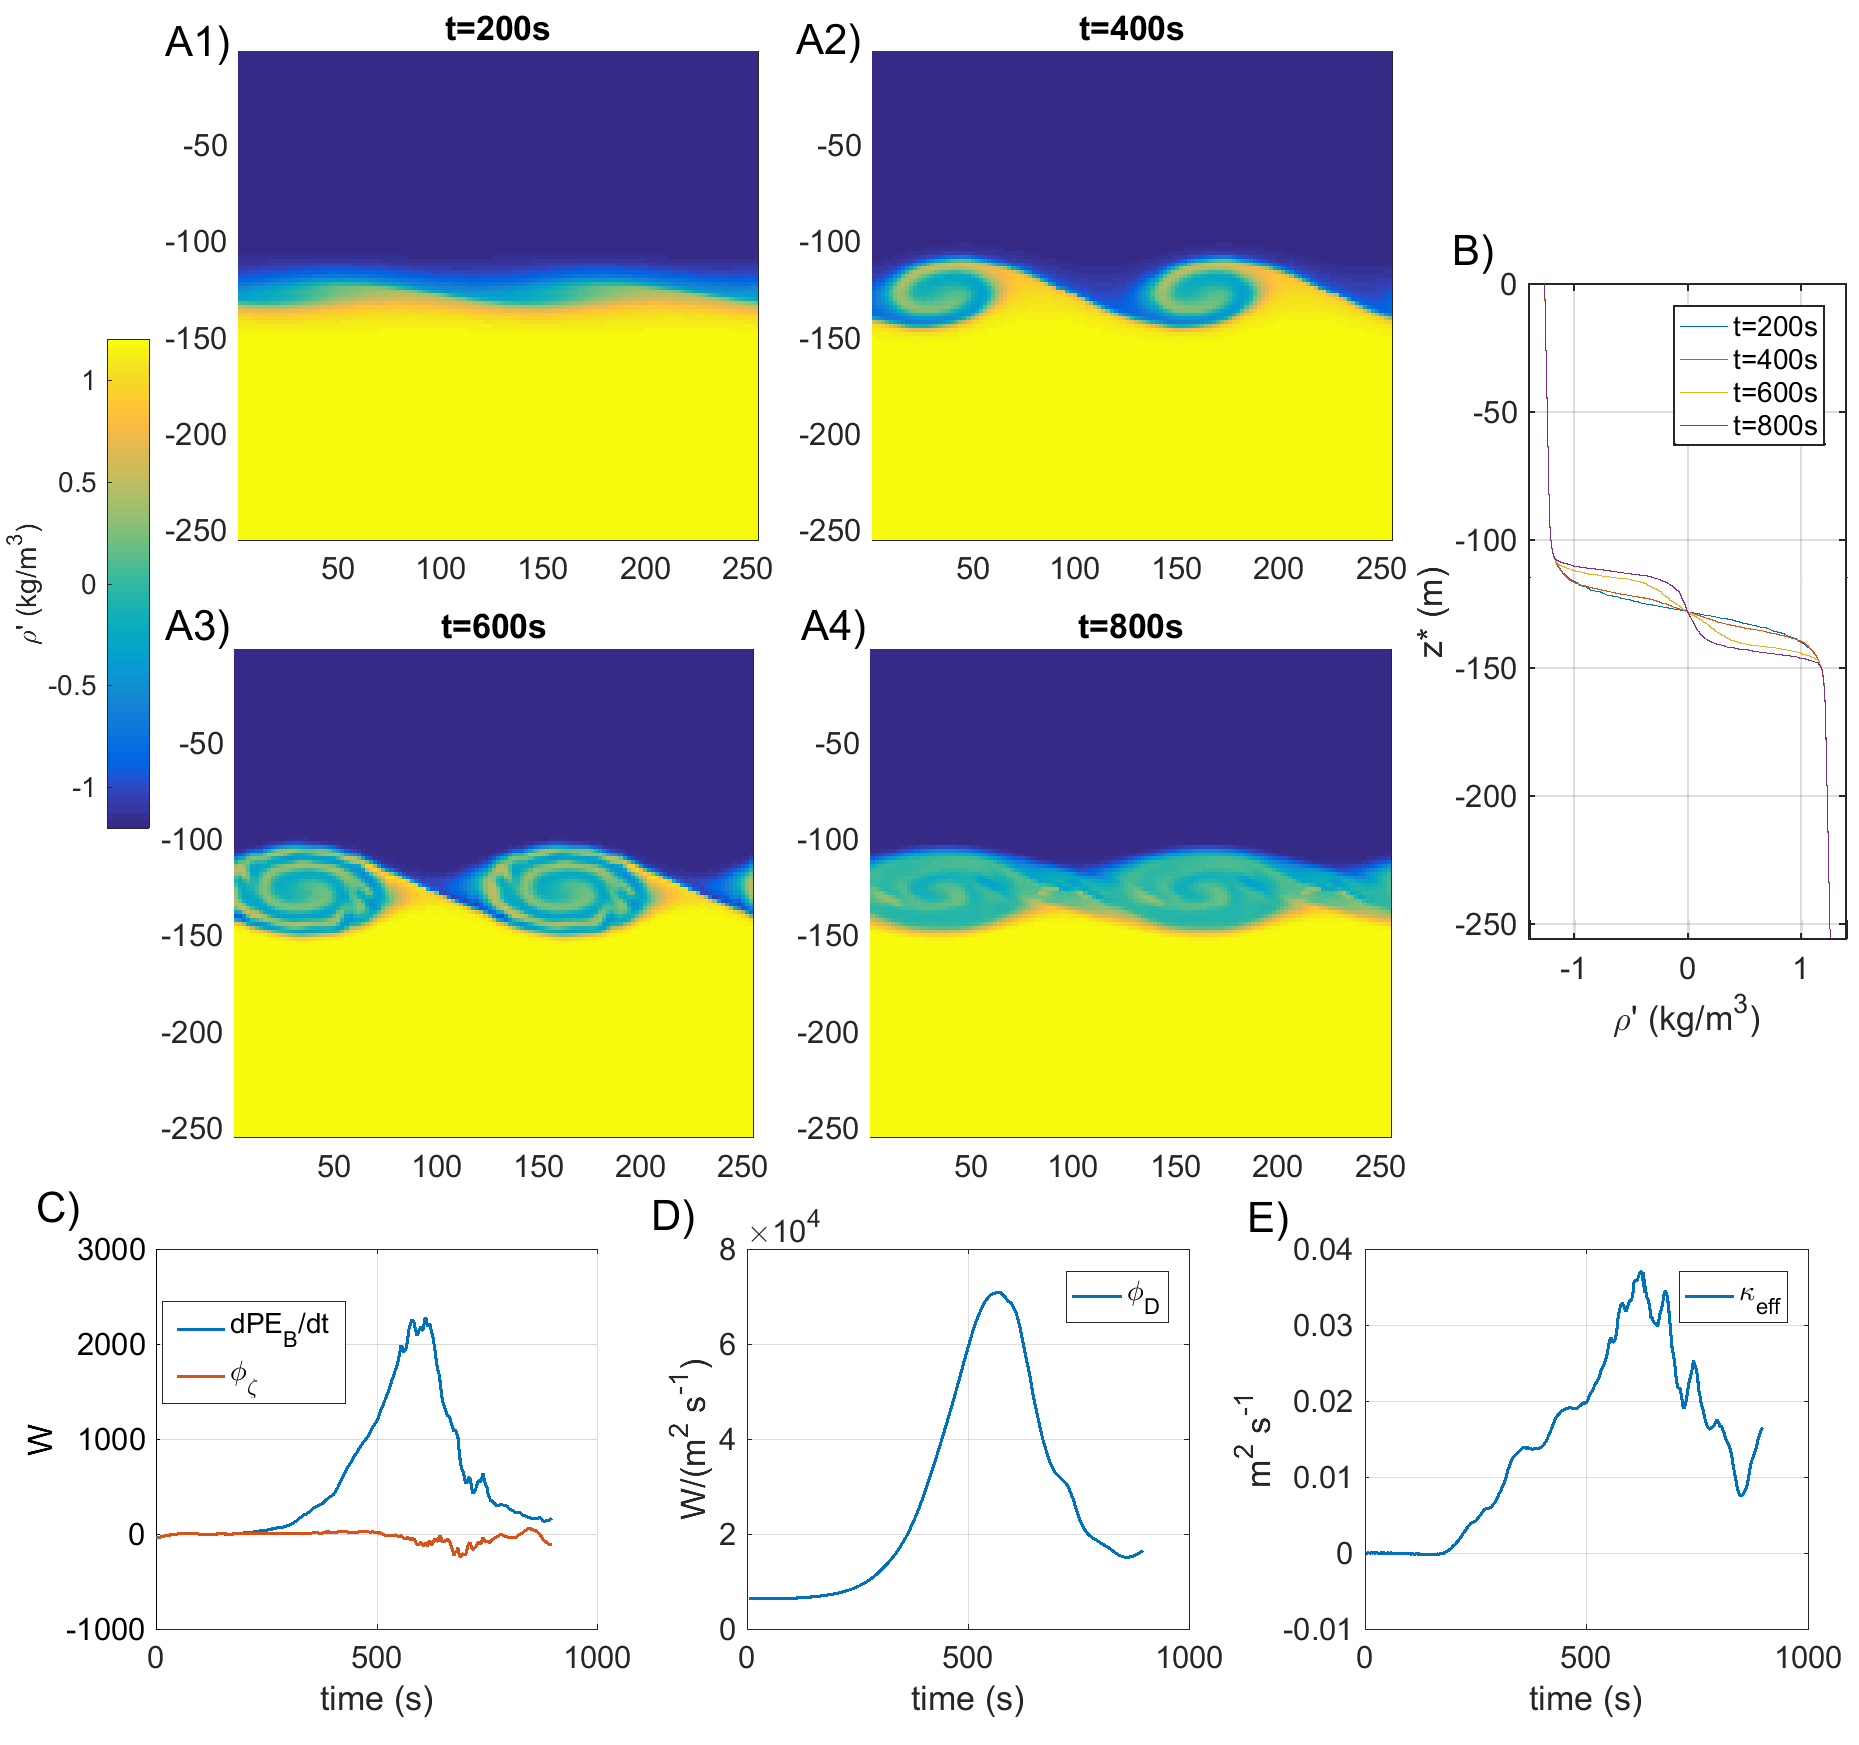
\includegraphics[width=1\textwidth]{./CHAP_BPE/Fig_KH2.png}
\caption[Tracer field and evaluation of $\kappa_{eff}$ for configuration $BPE_{kh}$]{(A1 to A4) Tracer field simulated in the $BPE_{kh}$ configuration for $t\ = \ 200,\ 400,\ 600,\ 800s$. (B1) Reference profile from the rearrangement of the tracer field at the same times in the simulation. (C, D and E) Evaluation of the time evolution of some terms of the balance equation \ref{bilanBPEal} over the whole simulated domain.}
\label{figCkh}
\end{figure}
% dx$=$dz$=$2m,$\rho_0 = 1034kg/m^3$ ,amplitude cisaillement courant initial 2m/s, cyclic in x, free surface, based on experiments of \citet{penney_2020}.
The initial field is a two-layer stratification  $\Delta \rho\  =\ 2.5\ kg/m^3$ and a two-layer sheared horizontal current with $\Delta U\ =\ 2\ m/s$ in the vertical direction. Two unstable billows develop over the domain during the simulated period.\\
Figure (\noparref{figCkh}.A1-A4) show the evolution of the density field after $t = 200\ s,\ 400\ s,\ 600\ s$ and $800\ s$ and figure (\noparref{figCkh}.B) gives the evolution of the reference profile at the same times. The figures in the lower row provide the various terms involved in the BPE balance equation \ref{bilanBPEal}.\\
The surface-induced $\phi_{\zeta}$ term remains small compared to the others. The effective diffusivity $\kappa_{eff}$ increases significantly after 200 s as the Kelvin-Helmholtz instability and its associated billows develop. It reaches a maximal value after 600 s which coincides with the maximum amplitude of the diapycnal term $\phi_D$ and the higher shear and density gradients.
Once the Kelvin-Helmholtz instability has mixed the density field, the reference profile exhibits an intermediate homogeneous layer located between $z^*\ =\ 110\ m$ and $z^*\ =\ 140\ m$, which coincides with a decrease of the effective diffusivity $\kappa_{eff}$.

%%%%%%%%%%%%%%%%%%%%%%%%%%%%%%%%%%%%%%%%%%%%%
\subsection{Gibraltar strait configuration ($SimRef$)}
The induced mixing in the vertical section of Gibraltar strait is finally investigated in the simplest configuration of ocean flow in Gibraltar strait (SimRef) originally presented in chapter \ref{chapGBR2D}.\\
\begin{figure}[h!]
\centering
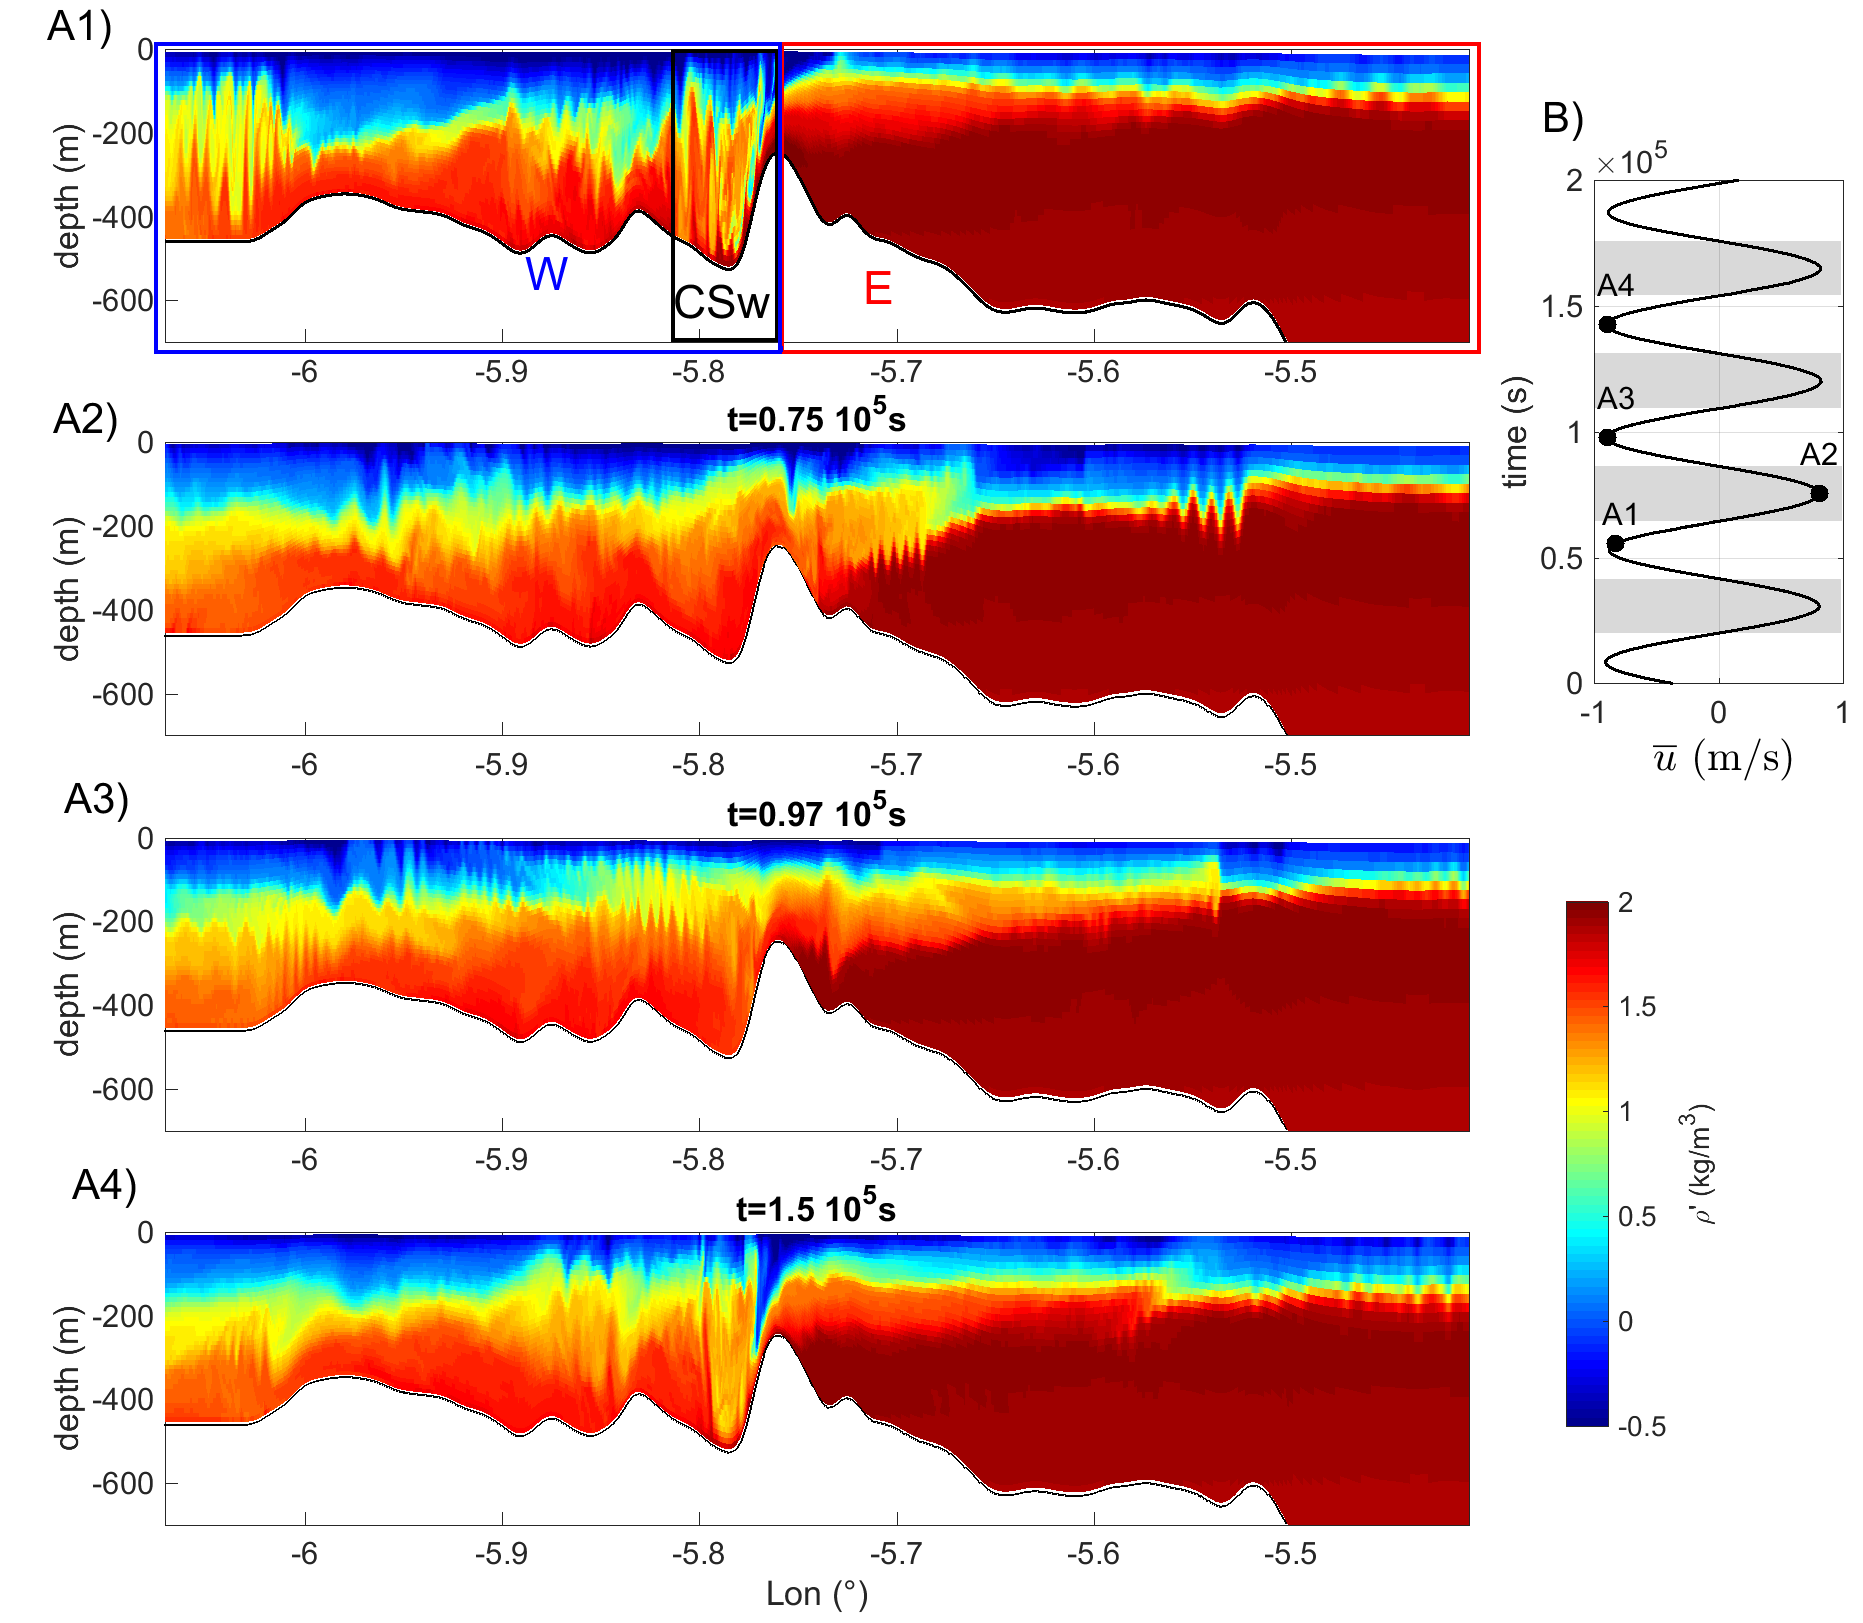
\includegraphics[width=1\textwidth]{./CHAP_BPE/Fig_Kappa_CS_ex.png}
\caption[Field of density anomaly in SimRef and definition of sub-domains.]{(A1 to A4) Simulated field of density anomaly $\rho'$ in simulation SimRef of chapter \ref{chapGBR2D} at various times. In (A1) definition of the sub-domains for the rearrangements as carried to give the temporal evolution of figure \ref{figCgbr2d}. (B) Time evolution of the barotropic current over the shallowest point in the domain at Camarinal Sill, with black dots indicating the instant of figures (A1 to A4).}
\label{figCgbr2d_ex}
\end{figure}
\begin{figure}[h!]
\centering
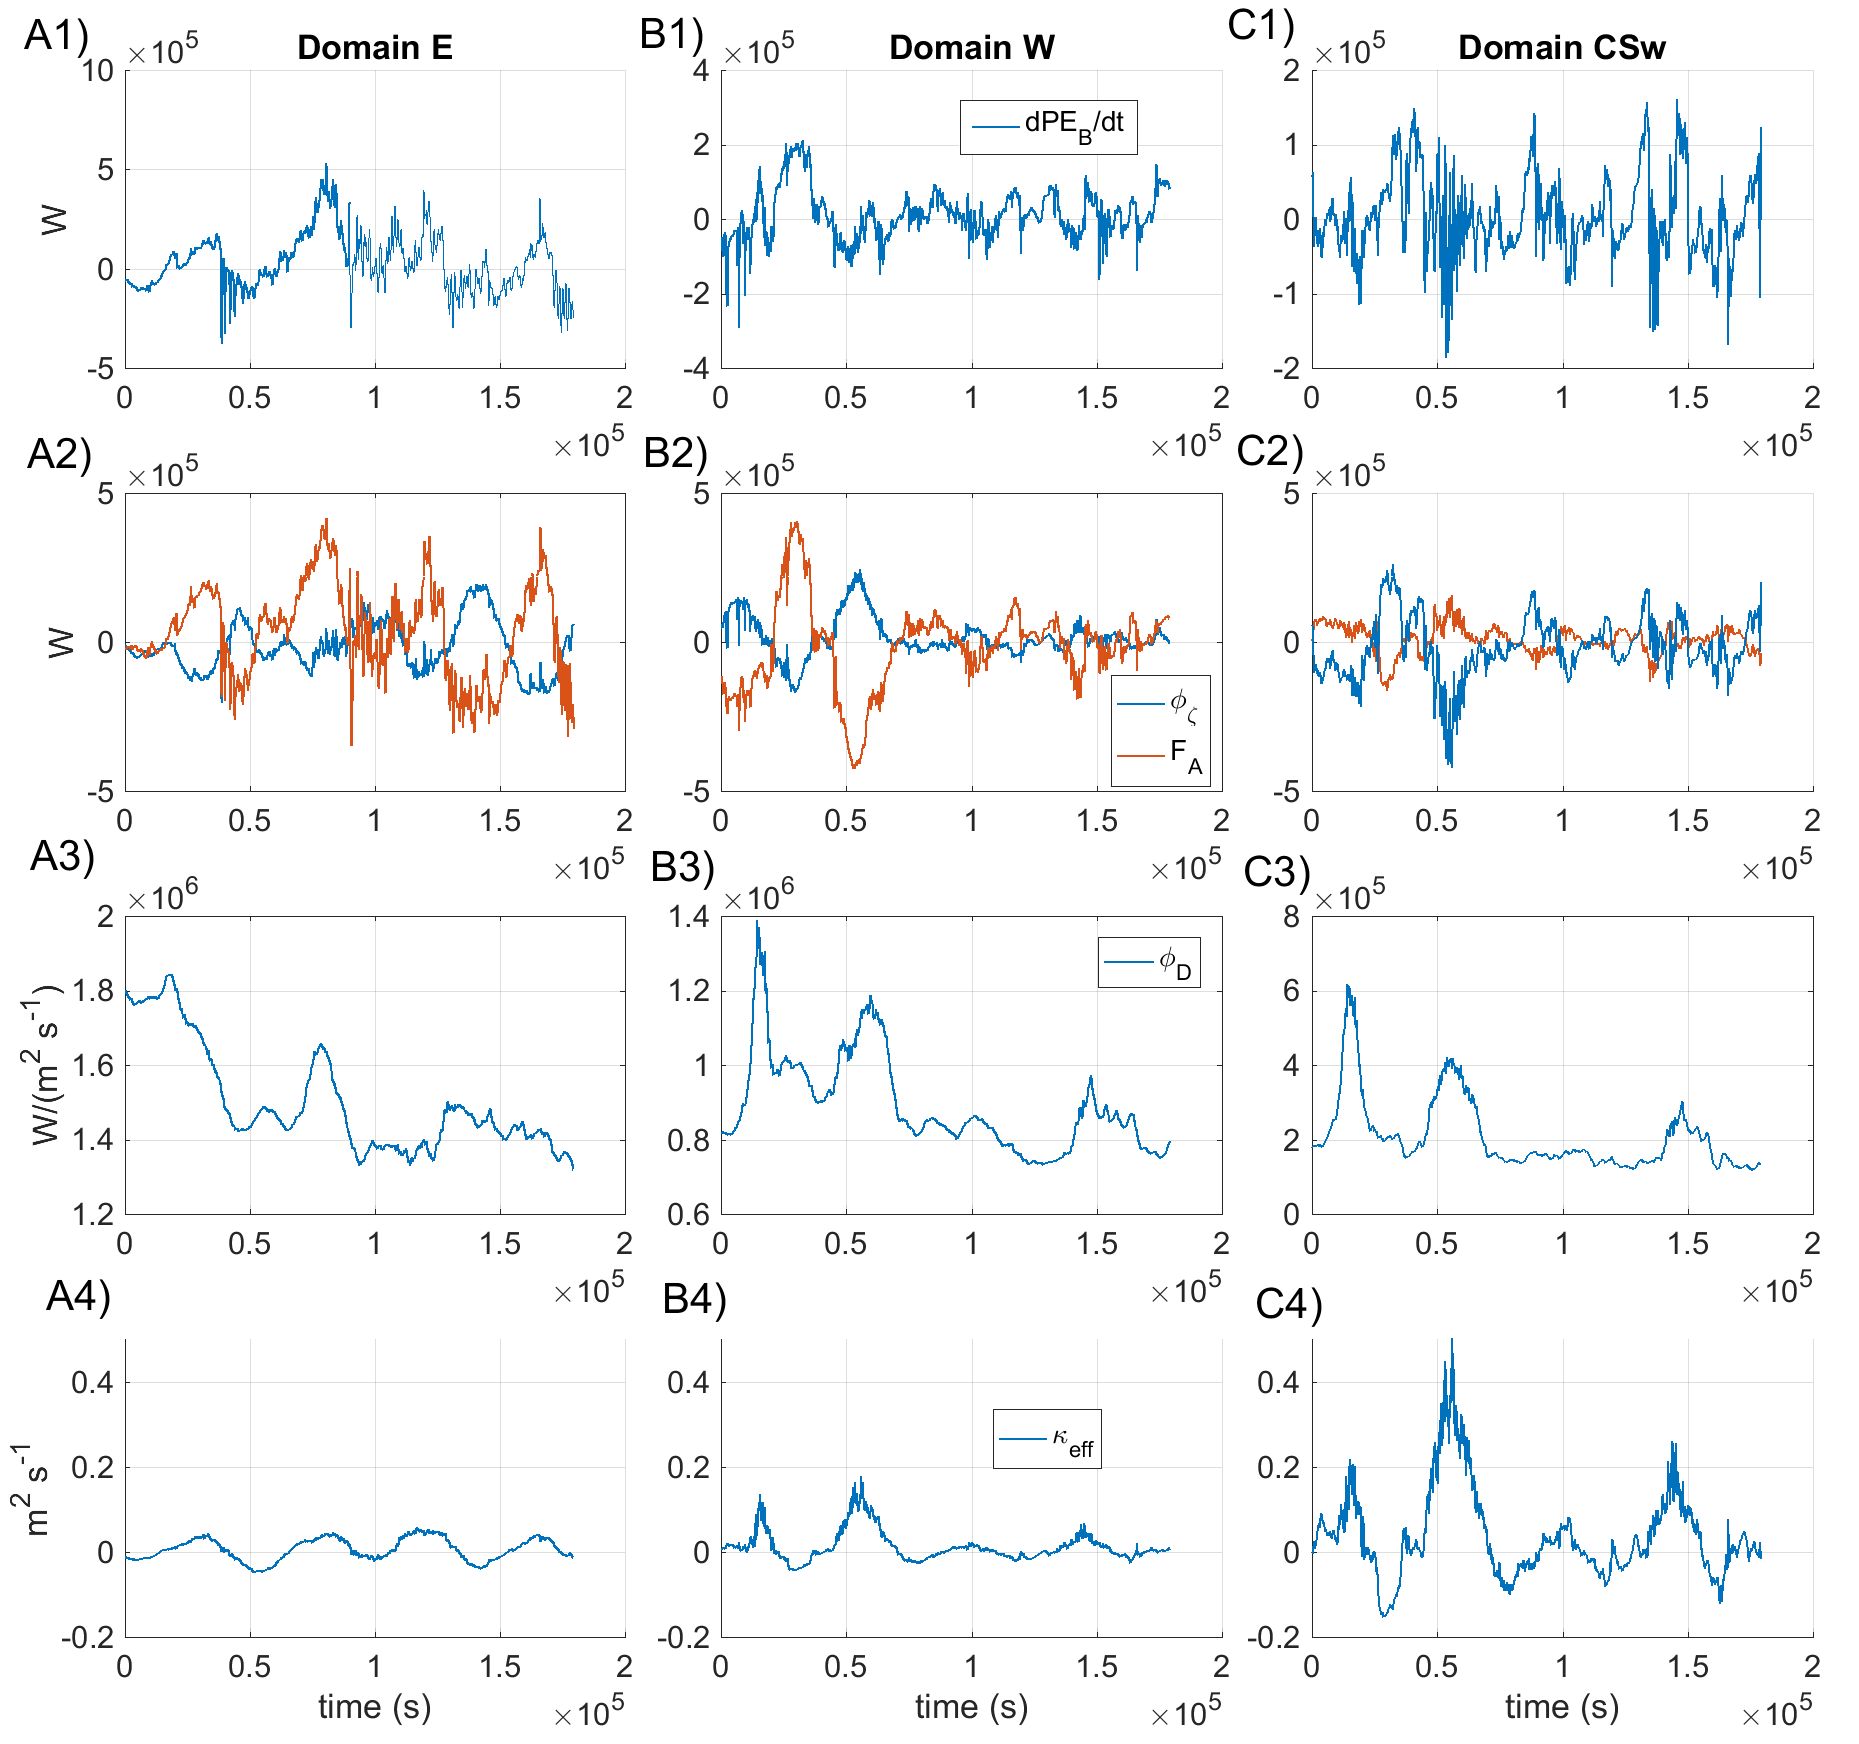
\includegraphics[width=1\textwidth]{./CHAP_BPE/Fig_Kappa_CS.png}
\caption[Evaluation of $\kappa_{eff}$ in different sub-domains of SimRef]{Evaluation of the time evolution of the terms of the balance equation \ref{bilanBPEal} in each domain of SimRef as defined in figure (\noparref{figCgbr2d_ex}.A1). Upper row is $dBPE/dt$, second row is $\phi_{\zeta}$ (blue) and $F_a$ (red), third row is $\phi_D$, bottom row is the evaluated $\kappa_{eff}$.}
\label{figCgbr2d}
\end{figure}
The initial time $(t\ =\ 0\ s)$ is now chosen for simulation time $t_{SimRef}\ =\ 6.29\ T$, i.e. at the beginning of the first outflow following the spin-up period whereas the simulation lasts $10.3\ T$ with $T\ =\ 12.4\ h$ the period of semi-diurnal tide.\\
The BPE evolution equation is evaluated over sub-domains of limited extension (see figure \noparref{figCgbr2d_ex}), where fine-scale processes, large turbulence eddies and thus mixing are supposed to occur. Figure \ref{figCgbr2d} presents the evaluation of the effective diffusivity $\kappa_{eff}$ for each domain, along with the remaining terms of equation \ref{bilanBPEal}.\\ 
The evolution of $dPE_B/dt$ is a noisy signal, the "noise" being largely explained by the sum of the non-diffusive terms $F_a$ and $\phi_{\zeta}$. Those two terms have approximately the same amplitude. Diffusive fluxes through the lateral boundaries are negligible compared to the diapycnal flux $\phi_D$.\\
The evolution in time of the effective diffusivity $\kappa_{eff}$ is in contrast noise-free. In the eastern part of the domain (E), this evolution is sinusoidal of period $T$ in agreement with the evolution of barotropic currents: it is positive positive when the barotropic component of the current is positive.
In the western part of the domain (W) and in it sub-domain (CSw), this semi-diurnal periodicity is readily apparent, not as regular oscillations this time but rather as intermittent episodes (bursts) of higher (positive) effective diffusivity $\kappa_{eff}$ during outflows (when the barotropic component of the current is this time negative).

\section{Discussion and conclusion}
A complete analysis of the Background Potential Energy (BPE) evolution equation has been carried out in several test-configurations of increasing complexity, ending with an application to the real ocean in the region of the strait of Gibraltar. This analysis is based on original analytical developments (to our knowledge at least) to derive an as-complete-as-possible evolution equation of the Background Potential Energy for free-surface water columns (\S \noparref{section_PE_chap2}). Original developments have also been proposed to evaluate numerically this evolution in non-flat regions of the ocean simulated with terrain-following, s-coordinate numerical models. The efficiency of the proposed implementation of the BPE algorithm remains affordable in terms of computing costs and memory storage for the hierarchy of configurations proposed, but new approaches need to be implemented to compute the reference state \citep{saenz_estimating_2015} for 3D LES of more extended regions.

%For now, the results from our test-configurations show that When the reference profile $z^*$ is computed locally, the lateral boundary fluxes exchanged through the vertical boundary separating two neighboring domains do not balance each other. 

In a free-surface domain with opened lateral boundaries, advection and motion of the free surface make $PE_B=\iiint_V \rho g z^* d\tau$ evolve with the reorganisation of the mass field (through $F_a$) and with the change of the water-column volume (through $\phi_{\zeta}$). In most studied configurations, those two terms are of the same order of magnitude and are the largest contributions to $dPE_B/dt$. The effective diffusivity $\kappa_{eff}$ is found to complete the balance and thus reflects (or at least should reflect) diapycnal mixing: it quantifies the averaged turbulent mixing occurring over the domain of integration (a sum of water columns). 
This averaging effect is in part due to the choice of an homogeneous value of $\kappa_{eff}$ over the selected domain. 

Several assumptions could additionally be reconsidered or at least evaluated with care.

The isotropy of the effective diffusivity $(\kappa_h=\kappa_v=\kappa)$ should be reconsidered when the implicit numerical diffusion of the advection schemes is at stake: implicit diffusion is indeed added specifically along the advection direction and diffusivity is not isotropic anymore.

The evaluations of the effective diffusivity has been made offline which leads to an additional limitation. Indeed, if an open-boundary configuration is studied, the sampling frequency must be chosen with care and must in particular remain high enough not to induce numerical truncation or artefacts.


Another consequence of our protocol is that this effective diffusivity value has contributions on timescales similar to other dynamical processes, including ones that would not reflect diapycnal mixing (such as reaching negative values, indicating re-stratification periods, whereas mixing is supposed to be an irreversible process). This is in particular the case even when the rearrangement is made over small sub-domains, as the timescale of advection is usually small compared to the timescale of diffusive mechanisms. So, an instantaneous evaluation of effective diffusion would not reflect the dynamical adjustment of the advected structures due to mixing.

In the present study, the time-averaging of the effective diffusivity was used to retrieve coefficients representative of processes over extended time periods coherent with dissipation processes, but it may be more pertinent to integrate the time-averaging process to the balance equation itself.

%and over a period which must be long enough for the main underlying dynamical adjustments to be achieved (i.e. at least larger than the time-scale of the diapycnal fluxes).

Finally, this study only focuses on the APE/BPE subdivision of the gravitational potential energy of the ocean. More information on the underlying effects of the simulated dynamics on the evolution of BPE and diabatic mixing could be gathered by evaluating transfers with and between other energy compartments, such as the kinetic energy of the flow \citep{floor_energy_2011}.


\section{Appendices to \textit{The evolution equation of BPE}}

%%%%%%%%%%%%%%%%%%%%%%%%%%%%%%%%%%%%%%%%%%%%%%%%%%%%%%%%%%%%%%%%%%%%%%%%%%%%%
\subsection{Reynolds Theorem}
\label{annexe_reynolds}
%%%%%%%%%%%%%%%%%%%%%%%%%%%%%%%%%%%%%%%%%%%%%%%%%%%%%%%%%%%%%%%%%%%%%%%%%%%%%
\subsubsection{Flux through a surface}
%%%%%%%%%%%%%%%%%%%%%%%%%%%%%%%%%%%%%%%%%%%%%%%%%%%%%%%%%%%%%%%%%%%%%%%%%%%%%
Based on \citep{delhaye_thermohydraulique_2008}, let $\mathbf{v}_{\Sigma}$ be the velocity of a material surface in the fluid:
\begin{equation}
	\displaystyle
	\mathbf{v}_{\Sigma}=\frac{\partial \mathbf{x}}{\partial t}\bigg\rvert _{\Sigma}
\end{equation}
with $\mathbf{x}$ the position of the current point where the velocity is computed. This velocity is undetermined  since the tangential component is itself undetermined. Only its normal component $(\mathbf{n}_{\Sigma}.\mathbf{v}_{\Sigma})$ can be computed and isolated. This component is different from the vertical component of $\mathbf{v}_{\Sigma}$ of equation \ref{eq_vertvelcomp}.

Demonstrations and further expressions of the normal component can be found in \citet{griffies_fundamentals_2004}, \citet{griffies_elements_2012} and \citet{delhaye_thermohydraulique_2008}.
\begin{subequations}
  \begin{alignat}{2}
  \displaystyle 
  & \frac{\partial z}{\partial t}\bigg\vert_s &&=
  \frac{\partial s}{\partial t}\bigg\vert_z
  \frac{\partial z}{\partial s}\bigg\vert_t\\
  & &&=h\norm{\mathbf{\nabla}s}\mathbf{n}_{\Sigma}.
  \mathbf{v}_{\Sigma}
  \end{alignat}
\end{subequations}
Metric tensor formulations lead to:
\begin{subequations}
  \begin{alignat}{2}
 & dS_{\Sigma} &&= h\norm{\mathbf{\nabla}s} dS\\
 & h dS &&=\mathbf{n}_{\Sigma}.\mathbf{v}_{\Sigma}dS_{\Sigma}
  \end{alignat}
\end{subequations}
%See bellow how this formula is used to write Leibniz rule...

\subsubsection{Formulations of the Reynolds Transport Theorem (\& Leibniz Rule)}
\paragraph{Demonstration.}
The difficulty to compute:
\begin{equation}
 \displaystyle
 \frac{d}{dt} \iiint_{\mathcal{V}_M(t)} \rho A d\tau
\end{equation}
is due to the fact that for a general time-varying volume $\mathcal{V}(t)$ the differentiation cannot be taken through the internal sign. To do so, we can however consider a change of coordinates to volume-attached coordinates \citep{hirasaki_chapter_2021}. Let $\mathcal{J}$ be the Jacobian (determinant of the Jacobian matrix) of the change of variables from Cartesian coordinates $(\mathbf{x},t)$ to volume varying coordinates $(\boldsymbol{\xi},t)$. Integrating volume is $\mathcal{V}(t)=\mathcal{V}_{\xi}=\mathcal{V}_{\xi}(t)$.

Kinematic evolution of material particulate ("dilation kinematic theorem") is then nothing but Reynolds'transport theorem (which is equivalent to Leibniz derivation rule to 3D volumes) \citep{hirasaki_chapter_2021}. Caution: the demonstration given in \citep{hirasaki_chapter_2021} is for a material volume $\mathcal{V}_M$. As the demonstration is kinematic, it is generalized here to a general volume moving thought the fluid flow $(\mathcal{V}(t))$. This problem is dealt with in \cite{web_course_web_2021} (and further references are given in there).

As a consequence for a general volume $\mathcal{V}(t)$ moving at a 3D velocity $  \mathbf{v}_{\Sigma}$:
\begin{equation}
 \displaystyle
 \frac{dJ}{dt}=J \mathbf{\nabla}.\mathbf{v}_{\Sigma}
\end{equation}
which is reminiscent of the kinematic evolution of the specific volume of a fluid particle:
\begin{equation}
 \displaystyle
 \frac{d\tau}{dt}=\tau \mathbf{\nabla}.\mathbf{v}
\end{equation}
sometime written:
\begin{equation}
 \displaystyle
 \frac{d\delta\tau}{dt}=\delta\tau \mathbf{\nabla}.\mathbf{v}
\end{equation}
which is noting but the continuity equation written for the specific volume. With the natural change of variable, the derivation can enter the integral sign and:
\begin{subequations}
  \begin{alignat}{2}
  \displaystyle 
  & \frac{d}{dt} \iiint_{\mathcal{V}(t)} \rho A d\tau &&=
  \frac{D}{Dt} \iiint_{\mathcal{V}(t)} \rho A d\tau\\[4mm]
  & &&= \frac{D}{Dt} \iiint_{\mathcal{V}(t)} \rho A d\mathbf{x}\\[4mm]
  & &&=\frac{D}{Dt} \iiint_{\mathcal{V}_{\xi}} \rho A J d\boldsymbol{\xi}\\[4mm]
  & &&=\iiint_{\mathcal{V}_{\xi}} \frac{D\rho A}{Dt}  J d\boldsymbol{\xi}
  +\iiint_{\mathcal{V}_{\xi}} \rho A \frac{DJ}{Dt} d\boldsymbol{\xi}\\[4mm]
  & &&=\iiint_{\mathcal{V}_{\xi}} \frac{D\rho A}{Dt}  J d\boldsymbol{\xi}
  +\iiint_{\mathcal{V}_{\xi}} \rho A \mathbf{\nabla}. \mathbf{v}_{\Sigma}\ J d\boldsymbol{\xi}
  \end{alignat}
\end{subequations}
Following \cite{truesdell_classical_1960}, a more general formulation can thus be recovered for a time-dependant volume $\mathcal{V}(t)$ moving with a velocity $\mathbf{v}_{\Sigma}$:
\begin{subequations}
  \begin{alignat}{2}
  \displaystyle 
  &  \frac{d}{dt} \iiint_{\mathcal{V}(t)} \rho A d\tau && =
  \iiint_{\mathcal{V}(t)} \frac{D\rho A}{Dt}  d\boldsymbol{x}
  +\iiint_{\mathcal{V}(t)} \rho A \mathbf{\nabla}.\mathbf{v}_{\Sigma}\ d\mathbf{x}\\[4mm]
 & && =
  \iiint_{\mathcal{V}(t)} \frac{\partial \rho A}{\partial t}\bigg\rvert_{xz} d\tau
  %+ \varoiint_{\mathcal{V}(t)}\rho A \mathbf{v}.\mathbf{S}\\
  + \oiint_{\mathcal{S}(t)}\rho A   \mathbf{v}_{\Sigma}.\mathbf{n}_{\Sigma}dS_{Sigma}
  \end{alignat}
\end{subequations}
where:
\begin{equation}
 \displaystyle
 \frac{D\bullet}{Dt}=\frac{\partial \bullet}{\partial t}\bigg\vert_{\boldsymbol{\xi}}
 +  \mathbf{v}_{\Sigma}.\mathbf{\nabla}_{t,\boldsymbol{\xi}}\bullet
\end{equation}
This is the generalized (Reynolds) transport theorem or the generalized Leibnitz theorem. Caution: the derivative $D/Dt$ is associated to $  \mathbf{v}_{\Sigma}$.

\paragraph{Closed time-dependent volume $\mathcal{V}(t)$.} 
Several formulations of this kinematic theorem can be given:
\begin{subequations}
  \begin{alignat}{2}
  \displaystyle 
  & \frac{d}{dt} \iiint_{\mathcal{V}(t)} \rho A d\tau &&=
  \iiint_{\mathcal{V}(t)} \frac{\partial \rho A}{\partial t}\bigg\rvert_{xz} d\tau
  %+ \varoiint_{\mathcal{V}(t)}\rho A \mathbf{v}.\mathbf{S}\\
  + \oiint_{\mathcal{V}(t)}\rho A   \mathbf{v}_{\Sigma}.d\mathbf{S}\\[4mm]
  % Line 2:
  &  &&= \iiint_{\mathcal{V}(t)} \left(\frac{\partial \rho A}{\partial t}\bigg\rvert_{xz}
  +\mathbf{\nabla}.(\rho A   \mathbf{v}_{\Sigma}) \right) d\tau\\[4mm]
  % Line 3:
  &  &&= \iiint_{\mathcal{V}(t)} \left(\rho \frac{\partial A}{\partial t}\bigg\rvert_{xz}
  +A \frac{ \partial \rho }{\partial t}\bigg\rvert_{xz}
  +\rho   \mathbf{v}_{\Sigma}.\mathbf{\nabla}A 
  +A\mathbf{\nabla}.(\rho   \mathbf{v}_{\Sigma}) \right) d\tau\\[4mm]
  % Line 4:
  & &&=\iiint_{\mathcal{V}(t)} \rho \frac{DA}{Dt}  d\tau 
  +\iiint_{\mathcal{V}(t)} A \left( \frac{\partial \rho}{\partial t} \bigg\rvert_{xz}
  +\mathbf{\nabla}.(\rho  \mathbf{v}_{\Sigma})\right) \ d\tau
  \end{alignat}
\end{subequations}
This can also be written:
\begin{subequations}
  \begin{alignat}{2}
  \displaystyle 
  & \frac{d}{dt} \iiint_{\mathcal{V}(t)} \rho A d\tau &&=
   \iiint_{\mathcal{V}(t)} \left(\rho \frac{\partial A}{\partial t}\bigg\rvert_{xz}
  +A \frac{ \partial \rho }{\partial t}\bigg\rvert_{xz}
  +\rho   \mathbf{v}_{\Sigma}.\mathbf{\nabla}A 
  +A   \mathbf{v}_{\Sigma}.\mathbf{\nabla}\rho
  +A\rho\mathbf{\nabla}.  \mathbf{v}_{\Sigma} \right) d\tau\\[4mm]
  % Line 2:
  & &&=\iiint_{\mathcal{V}(t)} \rho \frac{DA}{Dt}  d\tau 
  +\iiint_{\mathcal{V}(t)} A \frac{D \rho}{D t} d\tau
  + \iiint_{\mathcal{V}(t)} \rho A\mathbf{\nabla}.  \mathbf{v}_{\Sigma} d\tau
  \end{alignat}
\end{subequations}
or alternatively:
\begin{subequations}
  \begin{alignat}{2}
  \displaystyle 
  & \frac{d}{dt} \iiint_{\mathcal{V}(t)} \rho A d\tau &&
  =\iiint_{\mathcal{V}(t)} \rho \frac{dA}{dt}  d\tau 
  +\iiint_{\mathcal{V}(t)} \left(A \frac{d \rho}{dt} 
  +\mathbf{\nabla}.\left[ \rho A(  \mathbf{v}_{\Sigma}-\mathbf{v})\right]
  +\rho A \mathbf{\nabla}.\mathbf{v} \right) d\tau\\[4mm]
  & &&
  =\iiint_{\mathcal{V}(t)} \rho \frac{dA}{dt}  d\tau 
  + \iiint_{\mathcal{V}(t)}\mathbf{\nabla}.\left[ \rho A(  \mathbf{v}_{\Sigma}-\mathbf{v})\right]d\tau
    \end{alignat}
\end{subequations}
where $  \mathbf{v}_{\Sigma}$ is defined as the velocity of the closed surface of $\mathcal{V}(t)$ and is more generally the 3D displacement velocity of the volume $\mathcal{V}(t)$.

 Caution: this has nothing to do with the velocity of the fluid in this volume except in the following particular case when considering a material volume, i.e. in the Lagrangian approach.
These general formulations and demonstrations are useful in s-coordinates.

\subsubsection{Material volume $\mathcal{V}_M(t)$ (kinematics \& dynamics)}
\paragraph{Formulation of the transport theorem.} 
A material volume $\mathcal{V}_M(t)$ is defined as a volume containing exactly the same fluid particles as time goes on.
Simplifications to obtain the simple expression of the integral variations in the case of a moving material volume are based on the use of the continuity equation or conservation of mass. 

As the control volume is advected by mean flow (Lagrangian approach), $  \mathbf{v}_{\Sigma}=\mathbf{v}$ :
\begin{equation}
  \displaystyle 
   \frac{d}{dt} \iiint_{\mathcal{V}_M(t)} \rho A d\tau =
  \iiint_{\mathcal{V}_M(t)} \rho \frac{dA}{dt}  d\tau 
  +\iiint_{\mathcal{V}_M(t)} A \frac{d \rho}{dt} d\tau
  +\iiint_{\mathcal{V}_M(t)} \rho A\mathbf{\nabla}.\mathbf{v} d\tau
\end{equation}
and thus:
\begin{subequations}
  \begin{alignat}{2}
  \displaystyle 
  & \frac{d}{dt} \iiint_{\mathcal{V}_M(t)} \rho A d\tau &&= \iiint_{\mathcal{V_M}(t)} \rho \frac{dA}{dt}  d\tau 
  +\iiint_{\mathcal{V}_M(t)} A \underbrace{\left( \frac{\partial \rho}{\partial t} \bigg\rvert_{xz}+\mathbf{\nabla}.(\rho\mathbf{v})\right)}_{=0} \ d\tau\\[4mm]
  & && = \iiint_{\mathcal{V}_M(t)} \rho \frac{dA}{dt}  d\tau 
  \end{alignat}
\end{subequations}
This is a generalization to 3D volume of the Leibniz rule. The time dependency of the integral volume $\mathcal{V}_M(t)$ is for a Lagrangian evolution with time-dependent boundaries. The present formulation is to be used for time-dependent boundaries whatever the velocity $  \mathbf{v}_{\Sigma}$ inside the volume.

\paragraph{Material volume $\mathcal{V}_M(t)$ in Lagrangian material coordinates.} 
The same exact approach and demonstration can be carried out in the case of a material volume as in the general case.
Let in this case $\mathcal{J}$ be the Jacobian (determinant of the Jacobian matrix) of the change of variables from Cartesian coordinates $(\mathbf{x},t)$ to material coordinates $(\boldsymbol{\xi},t)$. Integrating volume is $\mathcal{V}(t)=\mathcal{V}_{\xi}$.\\
Kinematic evolution of material particle ("dilation kinematic theorem") reads \citep{hirasaki_chapter_2021}:
\begin{equation}
 \displaystyle
 \frac{dJ}{dt}=J \mathbf{\nabla}.\mathbf{v}
\end{equation}
which is reminiscent of the kinematic evolution of a control volume:
\begin{equation}
 \displaystyle
 \frac{d\tau}{dt}=\tau \mathbf{\nabla}.\mathbf{v}
\end{equation}
With this kinematic theorem:
\begin{subequations}
  \begin{alignat}{2}
  \displaystyle 
  & \frac{d}{dt} \iiint_{\mathcal{V}_M(t)} \rho A d\tau &&=
  \frac{d}{dt} \iiint_{\mathcal{V}_M(t)} \rho A d\mathbf{x}\\[4mm]
  & &&=\frac{d}{dt} \iiint_{\mathcal{V}_{s}} \rho A J d\boldsymbol{\xi}\\[4mm]
  & &&=\iiint_{\mathcal{V}_{\xi}} \frac{d\rho A}{dt}  J d\boldsymbol{\xi}
  +\iiint_{\mathcal{V}_{\xi}} \rho A \frac{dJ}{dt} d\boldsymbol{\xi}\\[4mm]
  & &&=\iiint_{\mathcal{V}_{\xi}} \frac{d\rho A}{dt}  J d\boldsymbol{\xi}
  +\iiint_{\mathcal{V}_{\xi}} \rho A \mathbf{\nabla}.\mathbf{v}\ J d\boldsymbol{\xi}
  \end{alignat}
\end{subequations}
This leads finally to:
\begin{subequations}
  \begin{alignat}{2}
  \label{dintdt_s}
  \displaystyle 
  & \frac{d}{dt} \iiint_{\mathcal{V}_M(t)} \rho A d\tau &&=
  \iiint_{\mathcal{V}_{\xi}}\left( \frac{\partial \rho A}{\partial t}   
  +\mathbf{\nabla}.( \rho A \mathbf{v})\right) J d\boldsymbol{\xi} \\[4mm]
  & && =\iiint_{\mathcal{V}_M(t)} \frac{\partial \rho A}{\partial t}\bigg\rvert_{xz} d\tau
  + \oiint_{\mathcal{V}_M(t)}\rho A \mathbf{v}.d\mathbf{S}
  \end{alignat}
\end{subequations}
Reynolds transport theorem is recovered for a material volume, understood as a volume containing  the same fluid particles. This last relation can be viewed as the difference between the time variation of the extensive variable inside the domaine and the advective flux through the "control" surface matching at time "t" with material volume.

\paragraph{Time-independant "control" volume $\mathcal{V}_0$.} 
In the particular case when the volume (and thus his surface) is independent of time, then $  \mathbf{v}_{\Sigma}=0$ and as a consequence:
\begin{equation}
 \displaystyle
 	\frac{d}{dt}\iiint_{\mathcal{V}_0} A d\tau = \iiint_{\mathcal{V}_0}\frac{\partial A}{\partial t} d\tau
\end{equation}

\subsection{Formulations based on total derivatives (toward Lagrangian relations...)}
Note that the continuity equation can be written:
\begin{equation}
	\displaystyle
	\frac{d\ \delta \tau}{dt}=\frac{\partial v_{k}}{\partial x_k} \delta\tau= \mathbf{\nabla}.\mathbf{v}\ \delta\tau
\end{equation}

and so for a closed, moving volume $\mathcal{V}(t)$:
\begin{subequations}
  \begin{alignat}{2}
  \displaystyle 
  & \frac{d}{dt} \iiint_{\mathcal{V}(t)} \rho A d\tau &&=  
  \iiint_{\mathcal{V}(t)} \rho \frac{DA}{Dt}  d\tau 
  +\iiint_{\mathcal{V}(t)} A \frac{D(\rho d\tau)}{Dt}\\[4mm]
  & && =  \iiint_{\mathcal{V}(t)} \rho \frac{DA}{Dt}  d\tau 
  + \iiint_{\mathcal{V}(t)} A \frac{D\rho}{Dt} d\tau
  +\iiint_{\mathcal{V}(t)} \rho A \frac{Dd\tau}{Dt}\\[4mm]
  & && = \iiint_{\mathcal{V}(t)} \rho \frac{DA}{Dt}  d\tau 
  +\iiint_{\mathcal{V}(t)} A \frac{D\rho}{Dt} d\tau
  +\iiint_{\mathcal{V}(t)} \rho A \mathbf{\nabla}.  \mathbf{v}_{\Sigma}\ d\tau \\[4mm]
  & && = \iiint_{\mathcal{V}(t)} \rho \frac{DA}{Dt}  d\tau 
  \end{alignat}
\end{subequations}
where $D\bullet/Dt=\partial \bullet/\partial t+  \mathbf{v}_{\Sigma}.\mathbf{\nabla}\bullet$. The last simplification is associated to the conservation of mass when written:
\begin{equation}
 \displaystyle
 \frac{D\rho}{Dt}=-\rho\mathbf{\nabla}.  \mathbf{v}_{\Sigma}
\end{equation}
If the volume is now a material volume and is thus advected by the mean flow (Lagrangian approach), $  \mathbf{v}_{\Sigma}=\mathbf{v}_M$ and $D./Dt =d./dt$ :
\begin{subequations}
  \begin{alignat}{2}
  \displaystyle 
  &  \frac{d}{dt} \iiint_{\mathcal{V}_M(t)} \rho A d\tau && = 
  \iiint_{\mathcal{V}_M(t)} \rho \frac{dA}{dt}  d\tau 
  +\iiint_{\mathcal{V}_M(t)} A \frac{d\rho}{dt} d\tau
  +\iiint_{\mathcal{V}_M(t)} \rho A \mathbf{\nabla}.\mathbf{v} d\tau\\[4mm]
  & && \left[ =\iiint_{\mathcal{V}_M(t)} \rho \frac{dA}{dt}  d\tau 
  +\iiint_{\mathcal{V}_M(t)} A  \underbrace{\left(\frac{\partial \rho}{\partial t} 
  +\underbrace{\mathbf{v}.\mathbf{\nabla}\rho+\rho \mathbf{\nabla}.\mathbf{v} }_{=\mathbf{\nabla}.(\rho\mathbf{v})}\right)}_{=0} d\tau \right]\\[4mm]
  & && = \iiint_{\mathcal{V}_M(t)} \rho \frac{dA}{dt}  d\tau 
  +\iiint_{\mathcal{V}_M(t)} A \underbrace{\left( -\rho \mathbf{\nabla}.\mathbf{v} + \rho \mathbf{\nabla}.\mathbf{v}\right)}_{=0} d\tau\\[4mm]
  & && = \iiint_{\mathcal{V}_M(t)} \rho \frac{dA}{dt}  d\tau 
  \end{alignat}
\end{subequations}
recovering  the results from the Eulerian approach and the previous more general formulation.

\subsubsection{Rate of change of integrals in s-coordinate}

In s-coordinates, the ocean column behaves as a material volume in the vertical direction but not in the horizontal direction where it a fixed-in-time control volume. For a volume associated to the s-coordinate grid: $  \mathbf{v}_{\Sigma}=\mathbf{v}_h+\mathbf{v}_z-\mathbf{v}_s$. This is the vertical velocity of the iso-s surfaces. The integration volume in s-coordinates is a sum of "waters columns" and is named $\mathcal{V}_s$. 

\paragraph{Kinematic-Dynamic evolution (Left-Hand-Side).}
In an Eulerian approach, the depth-to- surface integration can be carried out using \ref{mass_s} with $J=h(t,\mathbf{x},z)$:
\begin{subequations}
  \begin{alignat}{2}
  \displaystyle 
 	&\frac{d }{d t} \iiint_{\mathcal{V}_{s}} \rho A\ d\tau &&
   =\iiint_{\mathcal{V}_{s}} \frac{d \rho A }{d t}\ d\tau \\[4mm]
   & && = \iiint_{\mathcal{V}_{s}} \frac{\partial \rho A}{\partial t}d\tau
  + \iiint_{\mathcal{V}_{s}}\mathbf{\nabla}.( \rho A   \mathbf{v}_{\Sigma}) d\tau \\[4mm]
  & &&
   =\iiint_{\mathcal{V}_{s}} \frac{\partial \rho A}{\partial t}d\tau
 +\iint_{\mathcal{S}} \rho A\   \mathbf{v}_{\Sigma}.\mathbf{n}_{\Sigma}\ dS_{\Sigma}
  \end{alignat}
\end{subequations}
\cite{griffies_fundamentals_2004}, \cite{griffies_elements_2012} and \cite{delhaye_thermohydraulique_2008} provides a reformulation of the latest term in Cartesian coordinates:
\begin{equation}
%  \begin{alignat}{2}
  \displaystyle 
 	\frac{d }{d t} \iiint_{\mathcal{V}_{s}} \rho A\ d\tau
   =\iiint_{\mathcal{V}_{s}} \frac{\partial \rho A}{\partial t}\underbrace{d\tau}_{dxdydz}
 +\iint_{\mathcal{S}} \rho A\  \frac{\partial z}{\partial t}\bigg\vert_{s}\ \underbrace{dS}_{dxdy}
%  \end{alignat}
\end{equation}
using the central relation (2.121) of \citep{griffies_elements_2012} and in \S 6 of \citep{griffies_fundamentals_2004}:
\begin{equation}
 \displaystyle
  \mathbf{v}_{\Sigma}.\mathbf{n}_{\Sigma}\ dS_{\Sigma}= \frac{\partial z}{\partial t}\bigg\vert_{s}\ dS
\end{equation}
Since the ocean bottom boundary is supposed to remain stationary, this leads eventually to:
\begin{equation}
\label{eq_reyn_zeta}
%  \begin{alignat}{2}
  \displaystyle 
 	\frac{d }{d t} \iiint_{\mathcal{V}_{s}} \rho A\ d\tau 
   =\iiint_{\mathcal{V}_{s}} \frac{\partial \rho A}{\partial t}\underbrace{d\tau}_{dxdydz}
 +\iint_{\mathcal{S}_{surf}} \rho A\  \frac{\partial \zeta}{\partial t}\ \underbrace{dS}_{dxdy}
%  \end{alignat}
\end{equation}

\paragraph{Using the kinematic condition.}
Caution: to recover this relation based on the kinematic condition, one has to remember that $\mathbf{v}_{\Sigma}$ is indeterminate \citep{delhaye_thermohydraulique_2008}. Its component tangent to the iso-s surface depends in particular on the parametrization of this surface. The component orthogonal to this surface can however be computed. As a consequence, one has to consider the product $\mathbf{v}_{\Sigma}.\mathbf{n}_{\Sigma}$ rather than $\mathbf{v}_{\Sigma}$ alone. 

The previous relation can then be recovered writing:
\begin{subequations}
  \begin{alignat}{2}
  \displaystyle 
  % Line 2:
 &\frac{d }{d t} \iiint_{\mathcal{V}_{s}} \rho A\ d\tau &&=
 \iiint_{\mathcal{V}_{s}} \frac{\partial \rho A}{\partial t}d\tau
 +\iint_{\mathcal{S}} \rho A\   \mathbf{v}_{\Sigma}.\mathbf{n}_{\Sigma}\ dS_{\Sigma}\\[4mm]
&  &&=
 \iiint_{\mathcal{V}_{s}} \frac{\partial \rho A}{\partial t}d\tau
 +\iint_{\mathcal{S}_{surf}} \rho A\  ( \mathbf{u}_{\Sigma}-\mathbf{w}_{\Sigma}).\mathbf{n}_{\Sigma}\ dS_{\Sigma}\\[4mm]
&  &&=
 \iiint_{\mathcal{V}_{s}} \frac{\partial \rho A}{\partial t}d\tau
 +\iint_{\mathcal{S}_{surf}}  \frac{\rho A}{\norm{\mathbf{\nabla}s}}
 \left( \mathbf{\nabla}_z s.\mathbf{u}-\frac{h}{h}(\frac{\partial s}{\partial t}
 +\mathbf{\nabla}_z s.\mathbf{u})
 \right)\underbrace{\ dS_{\Sigma}}_{=\sqrt{1+S^2} dS}
 \end{alignat}
\end{subequations}
Since $h \norm{\mathbf{\nabla}s}=\sqrt{1+S^2}$, we can recover:
\begin{equation}
 \displaystyle
 \frac{d }{d t} \iiint_{\mathcal{V}_{s}} \rho A\ d\tau=
  \iiint_{\mathcal{V}_{s}} \frac{\partial \rho A}{\partial t}d\tau  
  +\iint_{\mathcal{S}_{surf}}  \rho A \frac{\partial s}{\partial t} dS
\end{equation}
Then knowing that:
\begin{subequations}
  \begin{alignat}{2}
 \displaystyle
&\frac{\partial s}{\partial t}&&=
\frac{\partial z}{\partial t}-
\frac{\partial \zeta}{\partial t}\\[4mm]
& &&=\frac{\partial \zeta}{\partial t}=\frac{\partial \zeta}{\partial t}\bigg\vert_s
 \end{alignat}
 we can conclude that:
\end{subequations}
\begin{equation}
 \displaystyle
 \frac{d }{d t} \iiint_{\mathcal{V}_{s}} \rho A\ d\tau=
  \iiint_{\mathcal{V}_{s}} \frac{\partial \rho A}{\partial t}d\tau  
  +\iint_{\mathcal{S}_{surf}}  \rho A \frac{\partial \zeta}{\partial t} dS
\end{equation}


\paragraph{In s-coordinates.} 
This result can also be recovered considering Reynolds transport theorem and the fact that $\mathbf{v}_{s}$ vanishes over both the bottom and surface boundaries\color{black}.
This latest formulation can be recovered from the expression in Cartesian coordinates since
\begin{equation}
  \displaystyle 
 	\frac{d }{d t} \iiint_{\mathcal{V}_{s}} \rho A\ d\tau  =
 	\iiint_{\mathcal{V}_{s}} \frac{\partial \rho A}{\partial t}d\tau
 +\iint_{\mathcal{S}} \rho A\  \frac{\partial z}{\partial t}\bigg\vert_s \ dS
\end{equation}
The first term on the right hand side can be rewritten:
\begin{subequations}
  \begin{alignat}{2}
  \displaystyle
 & \iiint_{\mathcal{V}_{s}} \frac{\partial \rho A}{\partial t}d\tau &&=
 \iiint_{\mathcal{V}_{s}} \left( \frac{\partial \rho A}{\partial t}\bigg \vert_s 
 -\frac{1}{h}\frac{\partial \rho A}{\partial s}\frac{\partial z}{\partial t}\bigg\vert_s \right) h \ ds dx dy\\[4mm]
 & &&=
 \iiint_{\mathcal{V}_{s}} \left( \frac{\partial \rho h A}{\partial t}\bigg \vert_s 
 -\rho A \frac{\partial h}{\partial t}\bigg\vert_s
 -\frac{\partial}{\partial s}\left(\rho A \frac{\partial z}{\partial t}\right) \bigg\vert_s
 +\rho A \underbrace{\frac{\partial^2 z}{\partial s\partial t}}_{\partial h/\partial t\vert_s}
 \right) ds dx dy
  \end{alignat}
\end{subequations}
Canceling the second, third and fourth terms together and using the Green-Ostrogradsky theorem lead to:
%\begin{subequations}
%  \begin{alignat}{2}
%  \displaystyle 
% 	&\frac{d }{d t} \iiint_{\mathcal{V}_{s}} \rho A\ d\tau  &&=
% \iiint_{\mathcal{V}_{s}} \left( \frac{\partial \rho h A}{\partial t}\bigg \vert_s 
% \pm\frac{1}{h}\frac{\partial}{\partial s}\left(\rho A \frac{\partial z}{\partial t}\right) \bigg\vert_s
% \right) h ds dx dy\\
% & &&= \iiint_{\mathcal{V}_{s}} \frac{\partial \rho h A}{\partial t}\bigg \vert_s h ds dx dy
%  \end{alignat}
%\end{subequations}
\begin{subequations}
  \begin{alignat}{2}
  \displaystyle 
 	&\frac{d }{d t} \iiint_{\mathcal{V}_{s}} \rho A\ d\tau  &&=
 \iiint_{\mathcal{V}_{s}} \left( \frac{\partial \rho h A}{\partial t}\bigg \vert_s 
 \pm \frac{\partial}{\partial s}\left(\rho A \frac{\partial z}{\partial t}\right) \bigg\vert_s
 \right) ds dx dy\\[4mm]
 & &&= \iiint_{\mathcal{V}_{s}} \frac{\partial \rho h A}{\partial t}\bigg \vert_s ds dx dy
  \end{alignat}
\end{subequations}

\paragraph{Lagrangian approach.} 
We can recover the relation for the evolution over a material volume such as a sum of water columns:
\begin{subequations}
  \begin{alignat}{2}
  \displaystyle 
  & \frac{d}{dt} \iiint_{\mathcal{V}_{s}} \rho A d\tau &&=
  \iiint_{\mathcal{V}_{s}} \rho \frac{d A}{dt} d\tau
  + \iiint_{\mathcal{V}_{s}}\mathbf{\nabla}.\left[ \rho A(  \mathbf{v}_{\Sigma}-\mathbf{v})\right] d\tau\\[4mm]
  & &&=
  \iiint_{\mathcal{V}_{s}} \rho \frac{d A}{dt} d\tau
  + \iint_{\mathcal{S}_{surf}} \rho A(\mathbf{v}_{\Sigma}-\mathbf{v}).\mathbf{n}_{\Sigma} dS_{\Sigma}
    \end{alignat}
\end{subequations}
\cite{griffies_fundamentals_2004} (page 140) further shows that, at the surface:
\begin{equation}
 \displaystyle
 \mathbf{n}_{\Sigma}.(\mathbf{v}_{\Sigma}-\mathbf{v})=\frac{h}{\sqrt{1+S^2}}\underbrace{\frac{d s}{dt}}_{=1/h\ w_s}
\end{equation}
and using $w_s=h\dot{s}$ thus:
\begin{subequations}
  \begin{alignat}{2}
  \displaystyle 
  & \frac{d}{dt} \iiint_{\mathcal{V}_{s}} \rho A d\tau &&=
  \iiint_{\mathcal{V}_{s}} \rho \frac{d A}{dt} d\tau
  +\iint_{\mathcal{S}_{surf}} \rho A  \underbrace{w_s}_{=0} dS
    \end{alignat}
\end{subequations}

%%%%%%%%%%%%%%%%%%%%%%%%%%%%
\subsection{Conservation of an extensive quantity in a free-surface ocean}
%%%%%%%%%%%%%%%%%%%%%%%%%%%
\label{sub_conservation_ins}

To develop diagnostics in a realistic free-surface ocean, the conservation or at least the evolution of a given property defined as $\mathcal{A}=\iiint_{\mathcal{V}(t)} \rho A d\tau$ where $A$ is a given specific\footnote{Specific: per unit mass of the flow.} property must be calculated in a region of the ocean with a varying upper surface. For a general time-dependent volume $\mathcal{V}(t)$ moving with a velocity $\mathbf{v}_{\Sigma}$, a formulation of the Reynolds transport theorem (or Leibnitz theorem) is given by \citet{truesdell_classical_1960} and reformulated in Appendix \ref{annexe_reynolds}:
\begin{subequations}
  \begin{alignat}{2}
  \displaystyle 
  &  \frac{d}{dt} \iiint_{\mathcal{V}(t)} \rho A d\tau && =
  \iiint_{\mathcal{V}(t)} \frac{D\rho A}{Dt}  d\boldsymbol{x}
  +\iiint_{\mathcal{V}(t)} \rho A \mathbf{\nabla}.\mathbf{v}_{\Sigma}\ d\mathbf{x}\\[4mm]
 & && =
  \iiint_{\mathcal{V}(t)} \frac{\partial \rho A}{\partial t}\bigg\rvert_{xz} d\tau
  %+ \varoiint_{\mathcal{V}(t)}\rho A \mathbf{v}.\mathbf{S}\\
  + \oiint_{\mathcal{S}(t)}\rho A   \mathbf{v}_{\Sigma}.\mathbf{n}_{\Sigma}dS_{\Sigma}
  \end{alignat}
\end{subequations}
with the material derivative $D/Dt$ here associated to $  \mathbf{v}_{\Sigma}$:
\begin{equation}
 \displaystyle
 \frac{D\bullet}{Dt}=\frac{\partial \bullet}{\partial t}\bigg\vert_{\boldsymbol{\xi}}
 +  \mathbf{v}_{\Sigma}.\mathbf{\nabla}_{t,\boldsymbol{\xi}}\bullet
\end{equation}
In oceanic configurations, $\mathcal{V}(t)$ can be chosen as $\mathcal{V}_s$, a sum of water columns. In the absence of shoaling processes, this volume's boundaries only move in the vertical direction with the elevation of the free-surface. It is then possible to express $\mathcal{A}$ in s-coordinates with the Jacobian of transformation equal to $\mathcal{J}=h$:
\begin{equation}
  \displaystyle 
 	\frac{d }{d t} \iiint_{\mathcal{V}_{s}} \rho A\ d\tau  =
 	\frac{d }{d t} \iiint_{\mathcal{V}_{s}} \rho A\ h ds dx_s dy_s
\end{equation}
In this case, with the definition of constant-$s$ surfaces, the boundaries of volume $\mathcal{V}_s$ are constant and the time-derivative can directly be applied through the integral as :
\begin{subequations}
  \begin{alignat}{2}
  \displaystyle 
   &\frac{d }{d t} \iiint_{\mathcal{V}_{s}} \rho A\ h ds dx_s dy_s && =
   \iiint_{\mathcal{V}_{s}} \frac{\partial h \rho A}{\partial t}\bigg \vert_s ds dx_s dy_s\\[4mm]
   & &&= \iiint_{\mathcal{V}_{s}} \rho h \frac{\partial A}{\partial t}\bigg \vert_s  ds dx_s dy_s + \iiint_{\mathcal{V}_{s}} A \frac{\partial \rho h}{\partial t}\bigg \vert_s ds dx_s dy_s
   \end{alignat}
\end{subequations}
This formulation is based on Reynolds transport theorem (see appendix \noparref{annexe_reynolds}).

To simplify notations and without any loss of generality, integrals should in the following be restricted to the $(x,z)$ vertical plane and subscript $s$ should be abandoned:
\begin{equation}
\displaystyle
\mathcal{A}=\int_x\int_{-1}^0\rho A\ hdx ds
\end{equation}
The conservation of mass in equation \ref{mass_s} and the formulation of evolution of $\rho$ in equation \ref{eq_diff_s} of appendix \ref{annexe_ocmod} can be used, leading to:
\begin{subequations}
  \begin{alignat}{2}
  \displaystyle 
   & \frac{d }{d t} \int_x\int_{-1}^0\rho A\ hds dx && = \int_x\int_{-1}^0 \frac{\partial A}{\partial t}\bigg \vert_s \rho h ds dx\\[4mm]
 & && \quad - \int_x \int_{-1}^0 A \frac{\partial \rho h u}{\partial x}\bigg\rvert_{ts} \ dx ds \\[4mm] 
 & && \quad - \int_x \int_{-1}^0 A \frac{\partial \rho v_s}{\partial s}\bigg\rvert_{tx} \ dx ds \\[4mm]
 & && \quad + \int_x \int_{-1}^0 A \frac{\partial}{\partial x} \bigg(h \kappa^h \frac{\partial \rho}{\partial x}\bigg\rvert_{ts}\bigg)_{ts} \ dx ds \\[4mm]
 & && \quad + \int_x \int_{-1}^0 A \frac{\partial}{\partial s} \bigg(\frac{\kappa^v}{h} \frac{\partial \rho}{\partial s}\bigg\rvert_{tx}\bigg)_{tx} \ dx ds 
   \end{alignat}
\end{subequations}
Various fluxes can be simplified in this expression:
\begin{subequations}
  \begin{alignat}{2}
&\frac{d }{d t}\int_x\int_{-1}^0 \rho A\ h ds dx =&&  \int_x \int_{-1}^0 \rho h \frac{\partial A}{\partial t}\bigg\rvert_{xs} \ dx ds\\[4mm]
 & && \quad - \int_x \int_{-1}^0 \frac{\partial \rho h A u}{\partial x}\bigg\rvert_{ts} \ dx ds
 + \int_x \int_{-1}^0\rho h u \frac{\partial A}{\partial x}\bigg\rvert_{ts} \ dx ds\\[4mm] 
 & && \quad - \int_x \int_{-1}^0 \frac{\partial \rho A v_s}{\partial s}\bigg\rvert_{tx} \ dx ds
 + \int_x \int_{-1}^0 \rho v_s \frac{\partial A}{\partial s}\bigg\rvert_{tx} \ dx ds \\[4mm]
 & && \quad + \int_x \int_{-1}^0 \frac{\partial}{\partial x} \bigg(h A \kappa^h \frac{\partial \rho}{\partial x}\bigg\rvert_{ts}\bigg)_{ts} \ dx ds 
 - \int_x \int_{-1}^0 h \kappa^h \frac{\partial A}{\partial x}\bigg\rvert_{ts} \frac{\partial \rho}{\partial x}\bigg\rvert_{ts} \ dx ds \\[4mm]
 & && \quad + \int_x \int_{-1}^0 \frac{\partial}{\partial s} \bigg( A \frac{\kappa^v}{h} \frac{\partial \rho}{\partial s}\bigg\rvert_{tx}\bigg)_{tx} \ dx ds 
 - \int_x \int_{-1}^0 \frac{\kappa^v}{h} \frac{\partial A}{\partial s}\bigg\rvert_{tx} \frac{\partial \rho}{\partial s}\bigg\rvert_{tx} \ dx ds 
  \end{alignat}
\end{subequations}
Integrating by parts the advective and diffusive flux integrals in both the vertical and horizontal directions finally leads to:
\begin{subequations}
\label{Aint}
  \begin{alignat}{2}
  \displaystyle 
  &\frac{d }{d t} \int_x \int_{-1}^0 \rho h A\ dx ds =&&
 %
 % Begin 5th line
 %
\quad  \int_x \int_{-1}^0 \rho h \frac{\partial A}{\partial t}\bigg\rvert_{ts} \ dx ds\\[4mm]
 & && \quad - \bigg[ \int_{-1}^0 \rho h A u \ ds\bigg]_{x}
 + \int_x \int_{-1}^0\rho h u \frac{\partial A}{\partial x}\bigg\rvert_{ts} \ dx ds\\[4mm] 
 & && \quad - \bigg[ \int_{x} \rho A v_s \ ds\bigg]_{0}^1
 + \int_x \int_{-1}^0 \rho v_s \frac{\partial A}{\partial s}\bigg\rvert_{ts} \ dx ds \\[4mm]
 & && \quad + \bigg[ \int_{-1}^0 h A \kappa^h \frac{\partial \rho}{\partial x}\bigg\rvert_{ts} \ ds \bigg]_{x}
 - \int_x \int_{-1}^0 h \kappa^h \frac{\partial A}{\partial x}\bigg\rvert_{ts} \frac{\partial \rho}{\partial x}\bigg\rvert_{ts} \ dx ds \\[4mm]
 & && \quad + \bigg[ \int_x A \frac{\kappa^v}{h} \frac{\partial \rho}{\partial s}\bigg\rvert_{tx} \ dx \bigg]_0^1
 - \int_x \int_{-1}^0 \frac{\kappa^v}{h} \frac{\partial A}{\partial s}\bigg\rvert_{tx} \frac{\partial \rho}{\partial s}\bigg\rvert_{tx} \ dx ds
   \end{alignat}
\end{subequations}
This latest relation can also be formulated as a function of $dA/dt$:
\begin{subequations}
  \begin{alignat}{2}
 %
 % Begin 6th line
 %
 &\frac{d }{d t} \int_x \int_{-1}^0 \rho h A\ dx ds &&= \quad  \int_x \int_{-1}^0 \rho h \frac{d A}{d t} \ dx ds\\[4mm]
 & && \quad - \bigg[ \int_{-1}^0 \rho h A u \ ds\bigg]_{x} - 0\\[4mm] 
 & && \quad + \bigg[ \int_{-1}^0 h A \kappa^h \frac{\partial \rho}{\partial x}\bigg\rvert_{ts} \ ds \bigg]_{x}
 - \int_x \int_{-1}^0 h \kappa^h \frac{\partial A}{\partial x}\bigg\rvert_{ts} \frac{\partial \rho}{\partial x}\bigg\rvert_{ts} \ dx ds \\[4mm]
 & && \quad + \bigg[ \int_x A \frac{\kappa^v}{h} \frac{\partial \rho}{\partial s}\bigg\rvert_{tx} \ dx \bigg]_0^1
 - \int_x \int_{-1}^0 \frac{\kappa^v}{h} \frac{\partial A}{\partial s}\bigg\rvert_{tx} \frac{\partial \rho}{\partial s}\bigg\rvert_{tx} \ dx ds 
  \end{alignat}
\end{subequations}
with $\bigg[ \int_{x} \rho A v_s \ ds\bigg]_{0}^1 = 0$ since $v_s$ is void at the bottom and top boundaries. 

%\subsection{S-coordinates}
%Integration over the water column whose surface is varying in time. 
%A key property is:
%\begin{equation}
% \displaystyle
% \frac{dh}{dt}(t,\mathbf{x},z)=\frac{d}{dt}\left( \frac{\partial z}{\partial s}\bigg\vert_{txy}\right)
% =\frac{\partial }{\partial s}\frac{dz}{dt}=\frac{\partial w}{\partial s}(t,\mathbf{x},z)
%\end{equation}
\color{black}